% SIAM Article Template
\documentclass[review,hidelinks,onefignum,onetabnum]{siamart220329}

% Information that is shared between the article and the supplement
% (title and author information, macros, packages, etc.) goes into
% ex_shared.tex. If there is no supplement, this file can be included
% directly.

% SIAM Shared Information Template
% This is information that is shared between the main document and any
% supplement. If no supplement is required, then this information can
% be included directly in the main document.


% Packages and macros go here
\usepackage{lipsum}
\usepackage{amsfonts}
\usepackage{graphicx}
\usepackage{epstopdf}
\usepackage{algorithmic}
\ifpdf
  \DeclareGraphicsExtensions{.eps,.pdf,.png,.jpg}
\else
  \DeclareGraphicsExtensions{.eps}
\fi

% Add a serial/Oxford comma by default.
\newcommand{\creflastconjunction}{, and~}

% Used for creating new theorem and remark environments
\newsiamremark{remark}{Remark}
\newsiamremark{hypothesis}{Hypothesis}
\crefname{hypothesis}{Hypothesis}{Hypotheses}
\newsiamthm{claim}{Claim}

% Sets running headers as well as PDF title and authors
\headers{A second order numerical methods for Reisz-Fractional Elliptic Equation on graded mesh }{Jianxing Han and Minghua Chen}

% Title. If the supplement option is on, then "Supplementary Material"
% is automatically inserted before the title.
\title{second-order error analysis for Fractional Laplacian via Riesz Derivatives on graded meshes\thanks{Submitted to the editors DATE.
}}

% Authors: full names plus addresses.
\author{Jianxing Han\thanks{School of Mathematics and Statistics, Lanzhou University, Lanzhou 730000, PR China
  (\email{hanjx2023@mail.lzu.edu.cn}).}
  \and Minghua Chen\thanks{School of Mathematics and Statistics, Lanzhou University, Lanzhou 730000, PR China 
  (\email{chen@mail.lzu.edu.cn}).}
}

\usepackage{amsopn}
\DeclareMathOperator{\diag}{diag}


%%% Local Variables: 
%%% mode:latex
%%% TeX-master: "ex_article"
%%% End: 


% Optional PDF information
\ifpdf
\hypersetup{
  pdftitle={Second-order numerical method for two-dimensional two-sided space fractional convection diffusion equation},
  pdfauthor={D. Doe, P. T. Frank, and J. E. Smith}
}
\fi

% The next statement enables references to information in the
% supplement. See the xr-hyperref package for details.

\externaldocument[][nocite]{ex_supplement}

% FundRef data to be entered by SIAM
%<funding-group specific-use="FundRef">
%<award-group>
%<funding-source>
%<named-content content-type="funder-name"> 
%</named-content> 
%<named-content content-type="funder-identifier"> 
%</named-content>
%</funding-source>
%<award-id> </award-id>
%</award-group>
%</funding-group>

\begin{document}

\maketitle

% REQUIRED
\begin{abstract}
  \textcolor{gray}{
    This is an example SIAM \LaTeX\ article. This can be used as a
    template for new articles.  Abstracts must be able to stand alone
    and so cannot contain citations to the paper's references,
    equations, etc.  An abstract must consist of a single paragraph and
    be concise. Because of online formatting, abstracts must appear as
    plain as possible. Any equations should be inline.
  }
\end{abstract}

% REQUIRED
\begin{keywords}
  example, \LaTeX
\end{keywords}

% REQUIRED
\begin{MSCcodes}
  68Q25, 68R10, 68U05
\end{MSCcodes}

\section{Introduction}
\textcolor{gray}{
  The introduction introduces the context and summarizes the
  manuscript. It is importantly to clearly state the contributions of
  this piece of work.
}

For \(\Omega=(0,2T)\), \(1<\alpha<2\),
\textcolor{orange}{suppose \(f\in C^\beta(\Omega), \beta>4-\alpha, \|f\|_{\beta}^{(\alpha/2)}<\infty\)}
\begin{equation} \label{eq:equation}
  \begin{cases}
    (-\Delta)^{\frac{\alpha}{2}} u(x) = f(x), & x \in \Omega                      \\
    u(x) = 0,                                 & x \in \mathbb{R} \setminus \Omega
  \end{cases}
\end{equation}
where
\begin{equation} \label{def:operator}
  (-\Delta)^{\frac{\alpha}{2}} u(x) = -\frac{\partial^\alpha u}{\partial |x|^\alpha}
  = -\kappa_\alpha \frac{d^2}{dx^2} \int_\Omega \frac{|x-y|^{1-\alpha}}{\Gamma(2-\alpha)}u(y) dy
\end{equation}
\begin{equation} \label{def:kappa}
  \kappa_\alpha = -\frac{1}{2\cos(\alpha\pi/2)} > 0
\end{equation}
\textcolor{blue}{and the solution \(u\in C^{\alpha/2}(\Omega)\).}

\section{Regularity}
\label{sec:regularity}
For any \(\beta > 0\), 
we use the standard notation \(C^\beta(\bar{\Omega}),  C^\beta(\mathbb{R})\), etc., for Hölder spaces
and their norms and seminorms.
When no confusion is possible, 
we use the notation \(C^\beta (\Omega)\) to refer to \(C^{k,\beta'} (\Omega)\), where \(k\) is the greatest integer such that \(k<\beta\) and where \(\beta' = \beta - k\).
The Hölder spaces \(C^{k, \beta'}(\Omega)\) are defined as the subspaces of \(C^k(\Omega)\) consisting of functions whose \(k\)-th order partial derivatives are locally Hölder continuous\cite{Gilbarg1977} with exponent \(\beta'\) in \(\Omega\),
where \(C^k(\Omega)\) is the set of all \(k\)-times continuously differentiable functions on open set \(\Omega\).



\textcolor{red}{
\begin{definition}[delta dependent norm \cite{ROSOTON2014275}]
  ...
\end{definition}
}

\textcolor{blue}{
  \begin{theorem} \label{thm:regularity-f}
    Let \(f\in C^\beta(\Omega), \beta>2\) be such that \(\|f\|_{\beta}^{(\alpha/2)}<\infty\), then for \(l=0, 1, 2\)
    \begin{equation}
      |f^{(l)}(x)| \le \|f\|_{\beta}^{(\alpha/2)} \begin{cases}
        x^{-l-\alpha/2}, & \text{if } 0 < x \le T \\ (2T-x)^{-l-\alpha/2}, & \text{if } T\le x < 2T
      \end{cases}
    \end{equation}
  \end{theorem}
}

\textcolor{orange}{
  \begin{theorem}[Regularity up to the boundary \cite{ROSOTON2014275}] \label{thm:regularity}
    Let \(\Omega\) be a bounded domain, and \(\beta>0\) be such that neither \(\beta\) nor \(\beta+\alpha\) is an integer. Let \(f \in C^\beta (\Omega)\) be such that\( \|f\|_{\beta}^{(\alpha/2)} < \infty\), and \(u \in C^{\alpha/2} (\mathbb{R}^n)\) be a solution of \cref{eq:equation}. Then, \(u \in C^{\beta+\alpha} (\Omega)\) and
    \begin{equation}
      \|u\|_{\beta+\alpha}^{(-\alpha/2)} \le C \left( \|u\|_{C^{\alpha/2}(\mathbb{R})} + \|f\|_{\beta}^{(\alpha/2)} \right)
    \end{equation}
  \end{theorem}
  \begin{corollary} \label{cor:regularity-u}
    Let $u$ be a solution of \eqref{eq:equation} on $\Omega$. Then, for any $x\in\Omega$ and \(l=0, 1, 2, 3, 4\)
    \begin{equation}
      |u^{(l)}(x)| \le \|u\|_{\beta+\alpha}^{(-\alpha/2)} \begin{cases}
        x^{\alpha/2-l}, & \text{if } 0 < x \le T \\ (2T-x)^{\alpha/2-l}, & \text{if } T\le x < 2T
      \end{cases}
    \end{equation}
  \end{corollary}
}


% The outline is not required, but we show an example here.

The paper is organized as follows. Our main results are in
\cref{sec:main},  experimental
results are in \cref{sec:experiments}.
Readers would better see \cref{sec:proof-convergence} before \cref{sec:proof-truncation-error} to avoid details.


\section{Numeric Format}
\label{sec:numformat}


\begin{equation} \label{def:xj}
  x_i = \begin{cases}
    T \left(\frac{i}{N}\right)^r   ,      & 0 \le i \le N  \\
    2T - T \left(\frac{2N-i}{N}\right)^r, & N \le i \le 2N
  \end{cases}
\end{equation}
where $r\ge 1$ .
And let
\begin{equation} \label{def:hj}
  h_j = x_{j} - x_{j-1}, \quad 1\le j \le 2N
\end{equation}

Let $\{\phi_j(x)\}_{j=1}^{2N-1}$ be standard hat functions, which are basis of the piecewise linear function space.
\begin{equation}
  \phi_j(x) = \begin{cases}
    \frac{1}{h_j} (x-x_{j-1}),      & x_{j-1} \le x \le x_{j} \\
    \frac{1}{h_{j+1}} (x_{j+1}-x) , & x_{j} \le x \le x_{j+1} \\
    0,                              & \text{otherwise}
  \end{cases}
\end{equation}
And then, we can approximate $u(x)$ with
\begin{equation}
  u_h(x) := \sum_{j=1}^{2N-1} u(x_j) \phi_j(x)
\end{equation}

For convience, we denote
\begin{equation} \label{def:Ih}
  I_h^{2-\alpha}(x_i) := \frac{1}{\Gamma(2-\alpha)}\int_{\Omega} |x_i-y|^{1-\alpha} u_h(y) dy
\end{equation}
And now, we can approximate the operator \eqref{def:operator} at $x_i$ with
\begin{equation} \label{def:Dhalpha}
  \begin{aligned}
    D_h^{\alpha} u_h(x_i) & := D_h^2 I_h^{2-\alpha}(x_i) \\
                          & =\frac{2}{h_{i} + h_{i+1}}
    \left( \frac{1}{h_{i}} I_h^{2-\alpha}(x_{i-1}) - \left( \frac{1}{h_{i}} + \frac{1}{h_{i+1}} \right) I_h^{2-\alpha}(x_{i}) + \frac{1}{h_{i+1}} I_h^{2-\alpha}(x_{i+1}) \right)
  \end{aligned}
\end{equation}
Finally, we approximate the equation \eqref{eq:equation} with
\begin{equation} \label{def:discrete_equation}
  -\kappa_\alpha D_h^{\alpha} u_h(x_i) = f(x_i), \quad 1\le i \le 2N-1
\end{equation}


The discrete equation \eqref{def:discrete_equation} can be written in matrix form
\begin{equation} \label{eq:equation_matrix}
  AU = F
\end{equation}
where $U$ is unknown, $F=(f(x_1), \cdots, f(x_{2N-1}))$.
The matrix $A$ is constructed as follows:
Since
\begin{equation}
  \begin{aligned} \label{eq:Ih}
    I_h^{2-\alpha}(x_i) & = \frac{1}{\Gamma(2-\alpha)} \int_{\Omega} |x_i-y|^{1-\alpha} u_h(y) dy                                                                     \\
                        & = \sum_{j=1}^{2N-1} \frac{1}{\Gamma(2-\alpha)} \int_{\Omega} |x_i-y|^{1-\alpha} u(x_j) \phi_j(y) dy                                         \\
                        & = \sum_{j=1}^{2N-1} u(x_j)  \frac{1}{\Gamma(2-\alpha)} \int_{x_{j-1}}^{x_{j+1}} |x_i-y|^{1-\alpha} \phi_j(y) dy                             \\
                        & = \sum_{j=1}^{2N-1} \frac{u(x_j)}{\Gamma(4-\alpha)}
    \left( \frac{|x_{i}-x_{j-1}|^{3-\alpha}}{h_{j}} -\frac{h_{j} + h_{j+1}}{h_{j}h_{j+1}}|x_i-x_{j}|^{3-\alpha} +  \frac{|x_{i}-x_{j+1}|^{3-\alpha}}{h_{j+1}} \right) \\
                        & =: \sum_{j=1}^{2N-1} \tilde{a}_{ij} \; u(x_j), \quad 0 \le i \le 2N
  \end{aligned}
\end{equation}
Then, substitute in \eqref{def:Dhalpha}, we have
\begin{equation}
  -\kappa_\alpha  D_h^{\alpha} u_h(x_i) = \sum_{j=1}^{2N-1} a_{ij} \; u(x_j)
\end{equation}
where
\begin{equation} \label{mat:aij}
  a_{ij} = -\kappa_\alpha \frac{2}{h_{i} + h_{i+1}}
  \left( \frac{1}{h_{i}} \tilde{a}_{i-1,j} - \left( \frac{1}{h_{i}} + \frac{1}{h_{i+1}} \right) \tilde{a}_{i,j} +  \frac{1}{h_{i+1}} \tilde{a}_{i+1, j} \right), \quad 1\le i \le 2N-1
\end{equation}


\section{Main results}
\label{sec:main}


Here we state our main results; the proof is
deferred to \cref{sec:proof-truncation-error} and \cref{sec:proof-convergence}.

\textcolor{orange}{
  Let's denote \(h=\frac{1}{N}\), we have
  \begin{theorem}[Truncation Error] \label{thm:truncation-error}
    If $f$ satisfy that $f\in C^\beta(\Omega), \beta>4-\alpha$, $\|f\|_{\beta}^{(\alpha/2)} < \infty, \alpha\in(1,2)$, 
    and $u(x)$ is a solution of the equation \eqref{eq:equation}, 
    where $\|u\|_{\beta+\alpha}^{(-\alpha/2)}<\infty$,
    then there exists  constants
    $C_1(T,\alpha, r, \|u\|_{\beta+\alpha}^{(-\alpha/2)}, \|f\|_{\beta}^{(\alpha/2)})$, 
    $C_2(T,\alpha, r,  \|u\|_{\beta+\alpha}^{(-\alpha/2)})$, such that
    the truncation error of the discrete format satisfies
    \begin{equation} \label{eq:truncation-error}
      \begin{aligned}
        \tau_i :=& | -\kappa_\alpha D_h^{\alpha} u_h(x_i) - f(x_i) | \\
        \le & C_1  h^{\min\{\frac{r\alpha}{2}, 2\}} \begin{cases}
                                                      x_i^{-\alpha},       & 1\le i\le N \\
                                                      (2T-x_i)^{-\alpha} , & N<i\le 2N-1
                                                    \end{cases} \\
            & + C_2(r-1) h^2
        \begin{cases}
          |T-x_{i-1}|^{1-\alpha}, \quad 1\le i\le N \\
          |T-x_{i+1}|^{1-\alpha} , \quad N<i\le 2N-1
        \end{cases}
      \end{aligned}
    \end{equation}
  \end{theorem}
}


\textcolor{blue}{
  \begin{theorem}[Convergence]\label{thm:convergence}
    The discrete equation \eqref{def:discrete_equation} has sulotion $U$,
    and there exists a positive constant $C=C(T,\alpha, r, \|u\|_{\beta+\alpha}^{(-\alpha/2)}, \|f\|_{\beta}^{(\alpha/2)})$
    such that the error between the numerial solution $U$ with the exact solution $u(x_i)$ satisfies
    \begin{equation} \label{eq:error}
      \max_{1\le i \le 2N-1} |U_i - u(x_i)| \le C h^{\min\{\frac{r\alpha}{2}, 2\}}
    \end{equation}
    That means the numerial method has convergence order ${\min\{\frac{r\alpha}{2}, 2\}}$.
  \end{theorem}
}



\section{Proof of \cref{thm:truncation-error}}
\label{sec:proof-truncation-error}

For convience, let's denote
\begin{equation}
  I^{2-\alpha}(x) = \frac{1}{\Gamma(2-\alpha)} \int_{\Omega} |x-y|^{1-\alpha} u(y) dy
\end{equation}
Then, the truncation error of the discrete format can be written as
\begin{equation} \label{eq:truncerrordepart}
  \begin{aligned}
    - \kappa_\alpha D_h^{\alpha} u_h(x_i) - f(x_i)
     & = -\kappa_\alpha (D_h^2 I_h^{2-\alpha}(x_i) - \frac{d^2}{dx^2} I^{2-\alpha}(x_i))                                      \\
     & = -\kappa_\alpha D_h^2 (I_h^{2-\alpha}-I^{2-\alpha})(x_i) - \kappa_\alpha (D_h^2 - \frac{d^2}{dx^2}) I^{2-\alpha}(x_i) \\
  \end{aligned}
\end{equation}


\subsection{Estimate of $-\kappa_\alpha (D_h^2 - \frac{d^2}{dx^2}) I^{2-\alpha} (x_i)$}

\textcolor{blue}{
  \begin{theorem} \label{lmm:trunerror2}
    There exits a constant $C=C(T,\alpha, r, \|f\|_{\beta}^{(\alpha/2)})$ such that
    \begin{equation}
      \left|-\kappa_\alpha (D_h^2 - \frac{d^2}{dx^2}) I^{2-\alpha} (x_i) \right| 
      \le C h^2 \begin{cases}
        x_i^{-\alpha/2-2/r} ,     & 1\le i\le N    \\
        (2T-x_i)^{-\alpha/2-2/r}, & N\le i\le 2N-1
      \end{cases}
    \end{equation}
  \end{theorem}
  \begin{proof}
    Since \(f\in C^2(\Omega)\) and
    \begin{equation}
      \frac{d^2}{dx^2} ( - \kappa_\alpha I^{2-\alpha}(x)) = f(x),  \quad x \in \Omega,
    \end{equation}
    we have \(I^{2-\alpha} \in C^4(\Omega)\).
    Therefore, using equation \eqref{eq:Dh2simd4} of \cref{lmm:Dh2simd2}, for \(1\le i\le 2N-1\), we have
    \begin{equation}
      \begin{aligned}
        -\kappa_\alpha (D_h^2 - \frac{d^2}{dx^2}) I^{2-\alpha} (x_i)
         & = \frac{h_{i+1}-h_{i}}{3} f'(x_i) \\
         & \quad + \frac{2}{h_i + h_{i+1}}\left(\frac{1}{h_i} \int_{x_{i-1}}^{x_{i}} f''(y) \frac{(y-x_{i-1})^3}{3!} dy + \frac{1}{h_{i+1}} \int_{x_{i}}^{x_{i+1}} f''(y) \frac{(y-x_{i+1})^3}{3!} dy\right) \\
      \end{aligned}
    \end{equation}
    where \(\eta_1 \in [x_{i-1}, x_{i}], \eta_2 \in [x_{i}, x_{i+1}]\).
    By \cref{lmm:hi1-hi} and \cref{thm:regularity-f}  we have
    1.
    \begin{equation}
      \left| \frac{h_{i+1}-h_{i}}{3} f'(x_i) \right| \le \frac{C(r-1)\|f\|_{\beta}^{(\alpha/2)}}{3}  h^2 \begin{cases}
        x_i^{-\alpha/2-2/r} ,     & 1\le i\le N-1 \\
        0,                        & i=N           \\
        (2T-x_i)^{-\alpha/2-2/r}, & N<i\le 2N-1
      \end{cases}
    \end{equation}
    2.
    See \cref{prf:trucerr2d2f}, there is a constant \(C=C(T, \alpha, r, \|f\|_{\beta}^{\alpha/2})\) such that
    \begin{equation}
      \begin{aligned}
        %  & \left| \frac{1}{4!} \frac{2}{h_i + h_{i+1}} (h_i^3 f''(\eta_1) + h_{i+1}^3 f''(\eta_2)) \right| \\
        & \frac{2}{h_i + h_{i+1}}\left(\frac{1}{h_i} \int_{x_{i-1}}^{x_{i}} f''(y) \frac{(y-x_{i-1})^3}{3!} dy + \frac{1}{h_{i+1}} \int_{x_{i}}^{x_{i+1}} f''(y) \frac{(y-x_{i+1})^3}{3!} dy\right) \\
         & \quad \le C h^2 \begin{cases}
                             x_i^{-\alpha/2-2/r} ,     & 1\le i\le N    \\
                             (2T-x_i)^{-\alpha/2-2/r}, & N\le i\le 2N-1
                           \end{cases}
      \end{aligned}
    \end{equation}
    Summarizes, we get the result.
  \end{proof}
}


\subsection{Estimate of $R_i$}
\label{subsec:Ri}

Now, we study the first part of \cref{eq:truncerrordepart}
\begin{equation}
  \begin{aligned}
    D_h^2(I^{2-\alpha}-I_h^{2-\alpha})(x_i)
     & = D_h^2(\int_{0}^{2T}(u(y)-u_h(y)) \frac{|y-x_i|^{1-\alpha}}{\Gamma(2-\alpha)} dy) \\
  \end{aligned}
\end{equation}
For convience, let's denote
\begin{equation} \label{def:Tij}
  T_{ij} = \int_{x_{j-1}}^{x_{j}} (u(y) - u_h(y)) \frac{|y-x_i|^{1-\alpha}}{\Gamma(2-\alpha)} dy, \quad i=0, \cdots ,2N,\; j=1, \cdots , 2N
\end{equation}
And define
\begin{equation} \label{eq:Ri}
  \begin{aligned}
    R_i & := D_h^2(I^{2-\alpha}- I_h^{2-\alpha})(x_i)                                                                                                                                       \\
        & = \frac{2}{h_{i} + h_{i+1}}  \sum_{j=1}^{2N}  \left( \frac{1}{h_{i}}  T_{i-1,j} - \left(\frac{1}{h_{i}} + \frac{1}{h_{i+1}}\right)  T_{i,j} + \frac{1}{h_{i+1}} T_{i+1,j} \right), \quad 1\le i \le 2N-1
  \end{aligned}
\end{equation}


We have some results about the estimate of $R_i$
\textcolor{blue}{
  \begin{theorem} \label{thm:Ri-ilessN/2}
    For \(1\le i < N/2\), there exists $C=C(T, \alpha, r, \|u\|_{\beta+\alpha}^{(-\alpha/2)})$ such that
    \begin{equation}
      R_i \le \begin{cases}
        C h^2 x_i^{-\alpha/2-2/r} ,             & \alpha/2 - 2/r + 1 > 0 \\
        C h^2 (x_i^{-1-\alpha}\ln(i) + \ln(N)), & \alpha/2 - 2/r + 1 = 0 \\
        C h^{r\alpha/2+r} x_i^{-1-\alpha},        & \alpha/2 - 2/r + 1 < 0
      \end{cases}
    \end{equation}
  \end{theorem}
}
\textcolor{blue}{
  \begin{theorem} \label{thm:Ri-N/2le-i-leN}
    For \(N/2 \le i\le N\), there exists constant $C=C(T, \alpha, r, \|u\|_{\beta+\alpha}^{(-\alpha/2)})$ such that
    \begin{equation}
      R_i \le C(r-1) h^2|T-x_{i-1}|^{1-\alpha}  + \begin{cases}
        C h^2,             & \alpha/2-2/r+1 > 0 \\
        C h^2 \ln(N) ,     & \alpha/2-2/r+1 = 0 \\
        C h^{r\alpha/2+r}, & \alpha/2-2/r+1 < 0
      \end{cases}
    \end{equation}
  \end{theorem}
}

And for \(N<i\le 2N-1\), it is symmetric to the previous case.

To prove these results, we need some utils.
Also for simplicity, we denote
\begin{definition}
  \begin{equation}
    S_{ij} =  \frac{2}{h_{i} + h_{i+1}}  \left( \frac{1}{h_{i}}  T_{i-1,j} - \left(\frac{1}{h_{i}} + \frac{1}{h_{i+1}}\right)  T_{i,j} + \frac{1}{h_{i+1}} T_{i+1,j} \right)
  \end{equation}
  then
  \begin{equation}
    R_i = \sum_{j=1}^{2N} S_{ij}
  \end{equation}
\end{definition}

\subsection{Proof of \cref{thm:Ri-ilessN/2}}

\textcolor{blue}{
  \begin{lemma} \label{lmm:sumSi-ilessN/2-2ip1-N}
    There exists a constant \(C=C(T, \alpha, r, \|u\|_{\beta+\alpha}^{(-\alpha/2)})\) such that for  \(1 \le i < N/2\),
    \begin{equation}
      \begin{aligned}
        \sum_{j=\max\{2i+1, i+3\}}^{N} S_{ij} \le C h^2 x_i^{-\alpha/2-2/r}
      \end{aligned}
    \end{equation}
  \end{lemma}
  \begin{proof}
    Let
    \textcolor{red}{
    \begin{equation*}
      K_y(x) = \frac{|y-x|^{1-\alpha}}{\Gamma(2-\alpha)}
    \end{equation*}
    }
    For  \(\max\{2i+1, i+3\} \le j \le N\), by \cref{lmm:Dyjleh2ya/2m2/r} and \cref{lmm:Dh2ymx1malecy1ma}
    \begin{equation}
      \begin{aligned}
        S_{ij} & = \int_{x_{j-1}}^{x_{j}}(u(y) - u_h(y)) D_h^2 K_y (x_i) dy \\
        % &\le C h^2 \int_{x_{j-1}}^{x_{j}} y^{\alpha/2-2/r} \frac{|y-x_{i+1}|^{-1-\alpha}}{\Gamma(-\alpha)} dy \\
               & \le C h^2 \int_{x_{j-1}}^{x_{j}} y^{\alpha/2-2/r} \frac{y^{-1-\alpha}}{\Gamma(-\alpha)} dy                       \\
               & = C h^2 \int_{x_{j-1}}^{x_{j}} y^{-\alpha/2-2/r-1} dy
      \end{aligned}
    \end{equation}
    Therefore,
    \begin{equation}
      \begin{aligned}
        \sum_{j=\max\{2i+1, i+3\}}^{N} S_{ij}
         & \le C h^2 \int_{x_{2i}}^{x_{N}} y^{-\alpha/2-2/r-1} dy                     \\
         & = \frac{C}{\alpha/2+2/r} h^2 ( x_{2i}^{-\alpha/2-2/r} - T^{-\alpha/2-2/r}) \\
         & \le \frac{C}{\alpha/2+2/r} 2^{r(-\alpha/2-2/r)} h^2 x_i^{-\alpha/2-2/r}
      \end{aligned}
    \end{equation}
  \end{proof}
}

\textcolor{blue}{
  \begin{lemma} \label{lmm:sumSi-ilessN/2-Np1-2N}
    Thert exists a constant \(C=C(T, \alpha, r, \|u\|_{\beta+\alpha}^{(-\alpha/2)})\) such that for  \(1 \le i < N/2\),
    \begin{equation}
      \begin{aligned}
        \sum_{j=N+1}^{2N} S_{ij}
        \le \begin{cases}
              C h^2,             & \alpha/2-2/r+1 > 0 \\
              C h^2 \ln(N) ,     & \alpha/2-2/r+1 = 0 \\
              C h^{r\alpha/2+r}, & \alpha/2-2/r+1 < 0
            \end{cases}
      \end{aligned}
    \end{equation}
  \end{lemma}
}
\begin{proof}
  For \(1 \le i < N/2, N+1\le j\le 2N-1\), by equation \cref{lmm:Dyjleh22T-y} and \cref{lmm:Dh2ymx1malecy1ma}
  \begin{equation*}
    \begin{aligned}
      S_{ij} & = \int_{x_{j-1}}^{x_{j}}(u(y) - u_h(y)) D_h^2 K_y (x_i) dy \\
             & \le \int_{x_{j-1}}^{x_{j}} C h^2 (2T-y)^{\alpha/2-2/r} y^{-1-\alpha} dy                                          \\
             & \le C h^2  T^{-1-\alpha} \int_{x_{j-1}}^{x_{j}} (2T-y)^{\alpha/2-2/r} dy
    \end{aligned}
  \end{equation*}
  \begin{equation}
    \begin{aligned}
      \sum_{j=N+1}^{2N-1} S_{ij}
       & \le C T^{-1-\alpha} h^2 \int_{x_{N}}^{x_{2N-1}} (2T-y)^{\alpha/2-2/r}  dy                       \\
       & \le CT^{-1-\alpha} h^2 \begin{cases}
                                  \frac{1}{\alpha/2-2/r+1} T^{\alpha/2-2/r+1},        & \alpha/2-2/r+1 > 0 \\
                                  \ln(T)-\ln(h_{2N}),                                 & \alpha/2-2/r+1 = 0 \\
                                  \frac{1}{|\alpha/2-2/r+1|} h_{2N}^{\alpha/2-2/r+1}, & \alpha/2-2/r+1 < 0
                                \end{cases} \\
       & = \begin{cases}
             \frac{C}{\alpha/2-2/r+1}T^{-\alpha/2-2/r} \; h^2,                & \alpha/2-2/r+1 > 0 \\
             CrT^{-1-\alpha} h^2 \ln(N),                                      & \alpha/2-2/r+1 = 0 \\
             \frac{C}{|\alpha/2-2/r+1|} T^{-\alpha/2-2/r} \; h^{r\alpha/2+r}, & \alpha/2-2/r+1 < 0
           \end{cases}
    \end{aligned}
  \end{equation}
  And by \cref{lmm:Dyj1}
  \begin{equation*}
    S_{i,2N} \le C T^{-1-\alpha} h_{2N}^{\alpha/2+1} = C T^{-\alpha/2} h^{r\alpha/2+r}
  \end{equation*}
  And when \(\alpha/2-2/r+1\ge 0\),
  \begin{equation*}
    h^{r\alpha/2+r} \le h^2
  \end{equation*}
  Summarizes, we get the result.
\end{proof}



For \(i=1, 2\).

\begin{lemma} \label{lmm:R1R2}
  By \cref{lmm:sumSij13} , \cref{lmm:sumSi-ilessN/2-2ip1-N}  and \cref{lmm:sumSi-ilessN/2-Np1-2N}   we get
  \begin{equation}
    \begin{aligned}
      R_1 & = \sum_{j=1}^{3} S_{1j} + \sum_{j=4}^{2N} S_{1j} \\
          & \le C h^2 x_1^{-\alpha/2-2/r} +
      \begin{cases}
        C h^2,             & \alpha/2-2/r+1 > 0 \\
        C h^2 \ln(N) ,     & \alpha/2-2/r+1 = 0 \\
        C h^{r\alpha/2+r}, & \alpha/2-2/r+1 < 0
      \end{cases}
    \end{aligned}
  \end{equation}
  \begin{equation}
    \begin{aligned}
      R_2 & = \sum_{j=1}^{4} S_{2j} + \sum_{j=5}^{2N} S_{2j} \\
          & \le C h^2 x_2^{-\alpha/2-2/r} +
      \begin{cases}
        C h^2,             & \alpha/2-2/r+1 > 0 \\
        C h^2 \ln(N) ,     & \alpha/2-2/r+1 = 0 \\
        C h^{r\alpha/2+r}, & \alpha/2-2/r+1 < 0
      \end{cases}
    \end{aligned}
  \end{equation}
\end{lemma}


For \(3\le i < N/2\), we have a new separation of \(R_i\), Let's denote \(k=\lceil\frac{i}{2}\rceil\).
\begin{equation}
  \begin{aligned}
    R_i
    = & \sum_{j=1}^{2N} \frac{2}{h_i + h_{i+1}}
    \left( \frac{1}{h_{i+1}} T_{i+1, j}
    - (\frac{1}{h_{i}}+\frac{1}{h_{i+1}}) T_{i,j}
    +  \frac{1}{h_{i}} T_{i-1, j} \right)                  \\
    = & \sum_{j=1}^{k-1} \frac{2}{h_i + h_{i+1}}
    \left( \frac{1}{h_{i+1}} T_{i+1, j}
    - (\frac{1}{h_{i}}+\frac{1}{h_{i+1}}) T_{i,j}
    +  \frac{1}{h_{i}} T_{i-1, j} \right)                  \\
      & + \frac{2}{h_i + h_{i+1}}
    \left( \frac{1}{h_{i+1}} (T_{i+1, k} +  T_{i+1, k+1})
    - (\frac{1}{h_{i}}+\frac{1}{h_{i+1}}) T_{i,k} \right)  \\
      & + \sum_{j=k+1}^{2i-1} \frac{2}{h_i + h_{i+1}}
    \left( \frac{1}{h_{i+1}} T_{i+1, j+1}
    - (\frac{1}{h_{i}}+\frac{1}{h_{i+1}}) T_{i,j}
    +  \frac{1}{h_{i}} T_{i-1, j-1} \right)                \\
      & + \frac{2}{h_i + h_{i+1}}
    \left( \frac{1}{h_{i}} (T_{i-1, 2i} +  T_{i-1, 2i-1})
    - (\frac{1}{h_{i}}+\frac{1}{h_{i+1}}) T_{i,2i} \right) \\
      & + \sum_{j=2i+1}^{2N} \frac{2}{h_i + h_{i+1}}
    \left( \frac{1}{h_{i+1}} T_{i+1, j}
    - (\frac{1}{h_{i}}+\frac{1}{h_{i+1}}) T_{i,j}
    +  \frac{1}{h_{i}} T_{i-1, j} \right)                  \\
    = & I_1 + I_2 + I_3 + I_4 + I_5
  \end{aligned}
\end{equation}
% where \(I_1\) makes sence only if \(i\ge 3\).



\textcolor{blue}{
  \begin{lemma} \label{lmm:Ri-I1}
    There exists a constant \(C=C(T, \alpha, r, \|u\|_{\beta+\alpha}^{(-\alpha/2)})\) such that for \(3\le i \le N, k=\lceil\frac{i}{2}\rceil\)
    \begin{equation}
      |I_1| = |\sum_{j=1}^{k-1} S_{ij}| \le \begin{cases}
        C h^2 x_i^{-\alpha/2-2/r} ,        & \alpha/2-2/r+1 > 0 \\
        C h^2 x_i^{-1-\alpha} \ln(i),      & \alpha/2-2/r+1 = 0 \\
        C h^{r\alpha/2+r} x_i^{-1-\alpha}, & \alpha/2-2/r+1 < 0
      \end{cases}
    \end{equation}
  \end{lemma}
}
\begin{proof}
  by \cref{lmm:Dyj1} , \cref{lmm:Dh2xmy1malecx1ma}
  \begin{equation}
    S_{i1} \le C x_1^{\alpha/2} x_1 x_i^{-1-\alpha} = C x_1^{\alpha/2+1} x_i^{-1-\alpha} = C T^{\alpha/2+1} h^{r\alpha/2+r} x_i^{-1-\alpha}
  \end{equation}
  For  \(2 \le j \le k-1\), by \cref{lmm:Dyjleh2ya/2m2/r} and \cref{lmm:Dh2xmy1malecx1ma}
  \begin{equation}
    \begin{aligned}
      S_{ij} & = \int_{x_{j-1}}^{x_{j}}(u(y) - u_h(y)) D_h^2 K_y(x_i) dy \\
             & \le C h^2 \int_{x_{j-1}}^{x_{j}} y^{\alpha/2-2/r} \frac{x_i^{-1-\alpha}}{\Gamma(-\alpha)} dy                     \\
             & = C h^2 x_i^{-1-\alpha} \int_{x_{j-1}}^{x_{j}} y^{\alpha/2-2/r} dy
    \end{aligned}
  \end{equation}
  Therefore,
  \begin{equation}
    \begin{aligned}
      I_1 & = \sum_{j=1}^{k-1} S_{ij} = S_{i1} + \sum_{j=2}^{k-1} S_{ij}                                                                 \\
          & \le C h^{r\alpha/2+r} x_i^{-1-\alpha} + C h^2 x_i^{-1-\alpha} \int_{x_1}^{x_{\lceil\frac{i}{2}\rceil-1}} y^{\alpha/2-2/r} dy \\
          & \le C h^{r\alpha/2+r} x_i^{-1-\alpha} + C h^2 x_i^{-1-\alpha} \int_{x_1}^{2^{-r} x_{i}} y^{\alpha/2-2/r} dy                  \\
      % &\le C h^{r\alpha/2+r} x_i^{-1-\alpha} + \frac{C}{\alpha/2-2/r+1} h^2 x_i^{-1-\alpha} (x_1^{\alpha/2-2/r+1} + (2^{-r} x_i)^{\alpha/2-2/r+1} )  \\
      % &\le C (h^{r\alpha/2+r} x_i^{-1-\alpha} + h^2 x_i^{-\alpha/2-2/r} )
    \end{aligned}
  \end{equation}
  But
  \begin{equation}
    \begin{aligned}
      \int_{x_1}^{2^{-r} x_{i}} y^{\alpha/2-2/r} dy
       & \le \begin{cases}
               \frac{1}{\alpha/2-2/r+1} (2^{-r} x_i)^{\alpha/2-2/r+1} , & \alpha/2-2/r+1 > 0 \\
               \ln(2^{-r} x_i) - \ln(x_1),                              & \alpha/2-2/r+1 = 0 \\
               \frac{1}{|\alpha/2-2/r+1|} x_1^{\alpha/2-2/r+1},         & \alpha/2-2/r+1 < 0
             \end{cases}
    \end{aligned}
  \end{equation}
  So we have
  \begin{equation}
    I_1 \le \begin{cases}
      \frac{C}{\alpha/2-2/r+1} h^2 x_i^{-\alpha/2-2/r} ,          & \alpha/2-2/r+1 > 0 \\
      C h^2 x_i^{-1-\alpha} \ln(i),                               & \alpha/2-2/r+1 = 0 \\
      \frac{C}{|\alpha/2-2/r+1|} h^{r\alpha/2+r} x_i^{-1-\alpha}, & \alpha/2-2/r+1 < 0
    \end{cases}
  \end{equation}
\end{proof}

\begin{definition}
  For convience, let's denote
  \begin{equation} \label{def:Vij}
    V_{ij} = \frac{2}{h_{i} + h_{i+1}}  \left( \frac{1}{h_{i+1}} T_{i+1, j+1} - \left(\frac{1}{h_{i}}+\frac{1}{h_{i+1}}\right)  T_{i,j} + \frac{1}{h_{i}} T_{i-1, j-1} \right)
  \end{equation}
\end{definition}

\textcolor{blue}{
  \begin{theorem} \label{Ri-I3-2lN/2}
    There exists a constant \(C=C(T, \alpha, r, \|u\|_{\beta+\alpha}^{(-\alpha/2)})\) such that for \(3\le i < N/2, k=\lceil\frac{i}{2}\rceil\),
    \begin{equation}
      I_3 = \sum_{j=k+1}^{2i-1} V_{ij} \le C h^2 x_i^{-\alpha/2-2/r}
    \end{equation}
  \end{theorem}
}

To estimete \(V_{ij}\), we need some preparations.
\begin{lemma} \label{lmm:Tijexpand}
  For \(y\in[x_{j-1}, x_{j}]\), we can rewrite \(y = x_{j-1} + \theta h_j = (1-\theta) x_{j-1} + \theta x_j =: y_j^\theta , \; \theta\in [0,1]\), by \cref{lmm:Dyj}
  \begin{equation}
    \begin{aligned}
      T_{ij} & = \int_{x_{j-1}}^{x_{j}} (u(y) - u_h(y)) \frac{|y-x_i|^{1-\alpha}}{\Gamma(2-\alpha)} dy  \\
             & = \int_{0}^{1} (u(y_j^\theta) - u_h(y_j^\theta)) \frac{|y_j^\theta-x_i|^{1-\alpha}}{\Gamma(2-\alpha)} h_j d\theta  \\
      %        & = \int_{x_{j-1}}^{x_{j}}
      % -\frac{\theta (1-\theta)}{2} h_j^2 u''(y_j^\theta)\frac{|y_j^\theta-x_i|^{1-\alpha}}{\Gamma(2-\alpha)} \\
      %        & \quad + \frac{\theta (1-\theta)}{3!} h_j^3 \frac{|y_j^\theta-x_i|^{1-\alpha}}{\Gamma(2-\alpha)} ((1-\theta)^2 u'''(\eta_{j1}^\theta) - \theta^2  u'''(\eta_{j2}^\theta)) d y_j^\theta \\
             & = \int_{0}^{1}
      -\frac{\theta (1-\theta)}{2} h_j^3 u''(y_j^\theta)\frac{|y_j^\theta-x_i|^{1-\alpha}}{\Gamma(2-\alpha)}   \\
             & \quad + \frac{\theta (1-\theta)}{3!} h_j^4 \frac{|y_j^\theta-x_i|^{1-\alpha}}{\Gamma(2-\alpha)} ( \theta^2 u'''(\eta_{j1}^\theta) - (1-\theta)^2 u'''(\eta_{j2}^\theta)) d\theta
    \end{aligned}
  \end{equation}
  where \(\eta_{j1}^\theta \in [x_{j-1}, y_j^\theta], \eta_{j2}^\theta \in [y_j^\theta, x_j]\).
\end{lemma}
Now Let's construct a series of functions to represent \(T_{ij}\).
\begin{definition} \label{def:yj-i}
  For \(2\le i,j\le N-1\),
  \begin{equation} \label{def:xi2yj-jlN}
    {y_{j-i}}(x) = (x^{1/r}+ Z_{j-i})^r, \quad Z_{j-i} = T^{1/r}\frac{j-i}{N}
  \end{equation}
  \begin{equation} \label{def:xi2yj-jlNt}
    {y_{j-i}^{\theta}}(x) = (1-\theta) {y_{j-1-i}}(x) + \theta {y_{j-i}}(x)
  \end{equation}
  \begin{equation} \label{def:hj-jlN}
    {h_{j-i}}(x) = {y_{j-i}}(x) - {y_{j-i-1}}(x)
  \end{equation}
  Now, we define
  \begin{equation} \label{def:Pj-itheta-jlN}
    {P_{j-i}^\theta}(x) = ({h_{j-i}}(x))^3 u''({y_{j-i}^\theta}(x)) \frac{|{y_{j-i}^\theta}(x)-x|^{1-\alpha}}{\Gamma(2-\alpha)}
  \end{equation}
  \begin{equation} \label{def:Qj-itheta-jlN}
    {Q_{j-i}^\theta}(x) = ({h_{j-i}}(x))^4 \frac{|{y_{j-i}^\theta}(x)-x|^{1-\alpha}}{\Gamma(2-\alpha)}
  \end{equation}
\end{definition}
And now we can rewrite \(T_{ij}\)
\begin{lemma} \label{lmm:Tij-express-as-int-of-function}
  For \(2\le i \le N, 2 \le j \le N\),
  \begin{equation}
    \begin{aligned}
      T_{ij} & = \int_{0}^{1} -\frac{\theta (1-\theta)}{2} {P_{j-i}^\theta}(x_i) d\theta    \\
             & + \int_{0}^{1} \frac{\theta (1-\theta)}{3!}{Q_{j-i}^\theta}(x_i)( \theta^2  u'''(\eta_{j,1}^\theta) - (1-\theta)^2 u'''(\eta_{j,2}^\theta)) d\theta
    \end{aligned}
  \end{equation}
\end{lemma}

Immediately, we can see from \eqref{def:Vij} that
\begin{lemma} \label{lmm:Vij-int}
  For \( 3 \le i,j \le N-1\),
  \begin{equation}
    \begin{aligned}
      V_{ij} & = \frac{2}{h_{i} + h_{i+1}}  \left( \frac{1}{h_{i+1}} T_{i+1, j+1} - \left(\frac{1}{h_{i}}+\frac{1}{h_{i+1}}\right)  T_{i,j} + \frac{1}{h_{i}} T_{i-1, j-1} \right)                                                      \\
             & = \int_{0}^{1} -\frac{\theta (1-\theta)}{2} D_h^2 P_{j-i}^\theta(x_i)  d\theta                                                                                                                                           \\
             & \quad +  \int_{0}^1 \frac{\theta^3 (1-\theta)}{3!} \frac{2}{h_{i} + h_{i+1}}\left( \frac{{Q_{j-i}^\theta}(x_{i+1}) u'''(\eta_{j+1,1}^\theta) - {Q_{j-i}^\theta}(x_{i}) u'''(\eta_{j,1}^\theta)}{h_{i+1}}\right)  d\theta \\
             & \quad -  \int_{0}^1 \frac{\theta^3 (1-\theta)}{3!} \frac{2}{h_{i} + h_{i+1}}\left( \frac{{Q_{j-i}^\theta}(x_{i}) u'''(\eta_{j,1}^\theta) - {Q_{j-i}^\theta}(x_{i-1}) u'''(\eta_{j-1,1}^\theta)}{h_{i}}\right)  d\theta   \\
             & \quad -  \int_{0}^1 \frac{\theta (1-\theta)^3}{3!} \frac{2}{h_{i} + h_{i+1}}\left( \frac{{Q_{j-i}^\theta}(x_{i+1}) u'''(\eta_{j+1,2}^\theta) - {Q_{j-i}^\theta}(x_{i}) u'''(\eta_{j,2}^\theta)}{h_{i+1}}\right)  d\theta \\
             & \quad +  \int_{0}^1 \frac{\theta (1-\theta)^3}{3!} \frac{2}{h_{i} + h_{i+1}}\left( \frac{{Q_{j-i}^\theta}(x_{i}) u'''(\eta_{j,2}^\theta) - {Q_{j-i}^\theta}(x_{i-1}) u'''(\eta_{j-1,2}^\theta)}{h_{i}}\right)  d\theta
    \end{aligned}
  \end{equation}
\end{lemma}


To estimate \(V_{ij}\), we first estimate \(D_h^2 P_{j-i}^\theta(x_i)\) , but
By \cref{lmm:Dh2simd2},
\begin{equation}
  D_h^2 {P_{j-i}^\theta}(x_i) = {P_{j-i}^\theta}''(\xi), \quad \xi\in [x_{i-1}, x_{i+1}]
\end{equation}
By Leibniz formula, we calculate and estimate the derivations of
\(h_{j-i}^3(x)\), \(u''(y_{j-i}^{\theta}(x)) \) and \(\frac{|{y_{j-i}^\theta}(x)-x|^{1-\alpha}}{\Gamma(2-\alpha)}\) separately.



Firstly, we have
\begin{lemma} \label{lmm:estimatesofhj-i3}
  There exists a constant \(C=C(T, r)\) such that
  For \(3\le i \le N-1, \lceil\frac{i}{2}\rceil+1 \le j \le \min\{2i-1, N-1\}\), \(\xi \in [x_{i-1}, x_{i+1}]\),
  \begin{gather}
    h_{j-i}^3(\xi) \le C h^{2} x_{i}^{2-2/r}  h_j \\
    (h_{j-i}^3(\xi))' \le C(r-1)  h^2  x_{i}^{1-2/r} h_{j} \\
    (h_{j-i}^3(\xi))'' \le C(r-1)  h^2  x_{i}^{-2/r} h_{j}
  \end{gather}
\end{lemma}
The proof of this theorem see \cref{lmm:dhj-i3le-Ch2xi1-2r} and \cref{lmm:d2hj-i3leh2xi-2r}

Second,
\begin{lemma} \label{lmm:estimatesofu2yj-itheta}
  There exists a constant \(C=C(T, \alpha, r, \|u\|_{\beta+\alpha}^{(-\alpha/2)})\) such that
  For \(3\le i \le N-1, \lceil\frac{i}{2}\rceil+1 \le j \le \min\{2i-1, N-1\}\), \(\xi \in [x_{i-1}, x_{i+1}]\),
  \begin{gather}
    u''(y_{j-i}^{\theta}(\xi)) \le C x_i^{\alpha/2-2}    \\
    (u''(y_{j-i}^{\theta}(\xi)))' \le C x_i^{\alpha/2-3} \\
    (u''(y_{j-i}^{\theta}(\xi)))'' \le C x_i^{\alpha/2-4}
  \end{gather}
\end{lemma}
The proof of this theorem see \cref{prf:estimatesofu2yj-itheta}

And Finally, we have
\begin{lemma} \label{lmm:estimatesofy-xi1-a}
  There exists a constant \(C=C(T, \alpha, r)\) such that
  For \(3\le i \le N-1, 1 \le j \le \min\{2i-1, N-1\}\), \(\xi \in [x_{i-1}, x_{i+1}]\),
  \begin{gather}
    |{y_{j-i}^\theta}(\xi)-\xi|^{1-\alpha} \le C | y_j^\theta - x_i|^{1-\alpha} \\
    (|{y_{j-i}^\theta}(\xi)-\xi|^{1-\alpha})' \le C | y_j^\theta - x_i|^{1-\alpha} x_i^{-1} \\
    (|{y_{j-i}^\theta}(\xi)-\xi|^{1-\alpha})'' \le C | y_j^\theta - x_i|^{1-\alpha} x_i^{-2}
  \end{gather}
  where \(y_j^\theta = \theta x_{j-1} + (1-\theta) x_{j}\)
\end{lemma}
The proof of this theorem see \cref{prf:estimatesofy-xi1-a}


\textcolor{blue}{
  \begin{lemma} \label{lmm:d2Pj-itle}
    There exists a constant \(C=C(T, \alpha, r, \|u\|_{\beta+\alpha}^{(-\alpha/2)})\) such that
    For \(3\le i \le N-1, \lceil\frac{i}{2}\rceil+1 \le j \le \min\{2i-1, N-1\}\),
    \begin{equation}
      D_h^2 {P_{j-i}^\theta}(x_{i}) \le C h^2 \frac{|y_j^\theta - x_i|^{1-\alpha}}{\Gamma(2-\alpha)} x_i^{\alpha/2-2-2/r} h_j
    \end{equation}
    where \(y_j^\theta = \theta x_{j-1} + (1-\theta) x_{j}\)
  \end{lemma}
  \begin{proof}
    Since
    \begin{equation}
      D_h^2 {P_{j-i}^\theta}(x_i) = {P_{j-i}^\theta}''(\xi), \quad \xi\in [x_{i-1}, x_{i+1}]
    \end{equation}
    From \eqref{def:Pj-itheta-jlN}, using Leibniz formula and \cref{lmm:estimatesofhj-i3}, \cref{lmm:estimatesofu2yj-itheta} and \cref{lmm:estimatesofy-xi1-a}
  \end{proof}
}

\textcolor{orange}{
  \begin{lemma} \label{lmm:dQj-itle}
    There exists a constant \(C=C(T, \alpha, r, \|u\|_{\beta+\alpha}^{(-\alpha/2)})\) such that for \(3\le i < N, k=\lceil\frac{i}{2}\rceil\). \\
    For \(k \le j \le \min\{2i-1, N-1\}\),
    \begin{equation}
      \begin{aligned}
        \frac{2}{h_{i} + h_{i+1}} & \left( \frac{{Q_{j-i}^\theta}(x_{i+1}) u'''(\eta_{j+1}^\theta) - {Q_{j-i}^\theta}(x_{i}) u'''(\eta_{j}^\theta)}{h_{i+1}}\right) \\
                                  & \le C h^2 \frac{|y_j^\theta - x_i|^{1-\alpha}}{\Gamma(2-\alpha)} x_i^{\alpha/2-2-2/r} h_j
      \end{aligned}
    \end{equation}
    And for \(k+1 \le j \le \min\{2i, N\}\),
    \begin{equation}
      \begin{aligned}
        \frac{2}{h_{i} + h_{i+1}} & \left( \frac{{Q_{j-i}^\theta}(x_{i}) u'''(\eta_{j}^\theta) - {Q_{j-i}^\theta}(x_{i-1}) u'''(\eta_{j-1}^\theta)}{h_{i}}\right) \\
                                  & \le C h^2 \frac{|y_j^\theta - x_i|^{1-\alpha}}{\Gamma(2-\alpha)} x_i^{\alpha/2-2-2/r} h_j
      \end{aligned}
    \end{equation}
    where \(\eta_{j}^\theta \in [x_{j-1}, x_{j}]\).
  \end{lemma}
}
proof see \cref{prf:dQj-itle}



\textcolor{blue}{
  \begin{lemma} \label{lmm:Vijleh2xma22r}
    There exists a constant \(C=C(T, \alpha, r, \|u\|_{\beta+\alpha}^{(-\alpha/2)})\)  such that for \(3\le i < N, k=\lceil\frac{i}{2}\rceil, k+1 \le j \le \min\{2i-1, N-1\}\),
    \begin{equation} \label{eq:estimateVij-int}
      \begin{aligned}
        V_{ij} & \le C h^2 \int_{0}^{1}  \frac{|y_j^\theta - x_i|^{1-\alpha}}{\Gamma(2-\alpha)} x_i^{\alpha/2-2-2/r} h_j d\theta \\
               & =  C h^2 \int_{x_{j-1}}^{x_{j}}  \frac{|y - x_i|^{1-\alpha}}{\Gamma(2-\alpha)} x_i^{\alpha/2-2-2/r} dy
      \end{aligned}
    \end{equation}
  \end{lemma}
}
\begin{proof}
  Since \cref{lmm:Vij-int}, by \cref{lmm:d2Pj-itle} and \cref{lmm:dQj-itle}, we get the result immediately.
\end{proof}


Now we can prove \cref{Ri-I3-2lN/2} using \cref{lmm:Vijleh2xma22r}, \(k=\lceil\frac{i}{2}\rceil\)
\begin{equation}
  \begin{aligned}
    I_3 & = \sum_{k+1}^{2i-1} V_{ij}
    \le C h^2 \int_{x_{k}}^{x_{2i-1}} \frac{|y - x_i|^{1-\alpha}}{\Gamma(2-\alpha)} x_i^{\alpha/2-2-2/r} dy                                                   \\
        & = C h^2 \left( \frac{|x_{k} - x_i|^{2-\alpha}}{\Gamma(3-\alpha)} + \frac{|x_{2i-1} - x_i|^{2-\alpha}}{\Gamma(3-\alpha)}\right) x_i^{\alpha/2-2-2/r} \\
        & \le C h^2 x_{i}^{2-\alpha} x_i^{\alpha/2-2-2/r} = C h^2 x_i^{-\alpha/2-2/r}
  \end{aligned}
\end{equation}


\textcolor{blue}{
  \begin{lemma} \label{lmm:DhPj-it}
    \begin{equation}
      D_h P_{j-i}^\theta(x_i) := \frac{P_{k-i}^\theta(x_{i+1}) - P_{k-i}^\theta(x_i)}{h_{i+1}} = {P_{j-i}^\theta}'(\xi), \quad \xi \in [x_{i}, x_{i+1}]
    \end{equation}
  \end{lemma}
  Then, for \(3\le i \le N-1\), \(k=\lceil\frac{i}{2}\rceil\),
  \begin{equation}
    D_h P_{k-i}^\theta(x_i) \le C h^2 x_i^{-\alpha/2-2/r} h_j
  \end{equation}
}
\begin{proof}
  Using Leibniz formula, by \cref{lmm:estimatesofhj-i3}, \cref{lmm:estimatesofu2yj-itheta} and \cref{lmm:estimatesofy-xi1-a}, we take \(j=k+1, i=i+1\), we get
  \begin{equation}
    \begin{aligned}
      D_h P_{k-i}^\theta(x_i) & \le C h^2 x_{i+1}^{\alpha/2-2/r-1} |y_{k+1}^\theta-x_{i+1}|^{1-\alpha} h_{j+1} \\
                              & \le C h^2 x_{i}^{\alpha/2-2/r-1} |y_{k}^\theta-x_{i}|^{1-\alpha} h_{j}         \\
                              & \le C h^2 x_{i}^{-\alpha/2-2/r} h_j
    \end{aligned}
  \end{equation}
\end{proof}

\textcolor{blue}{
  \begin{lemma} \label{lmm:Ri-I2-I4-ilN/2}
    There exists a constant \(C=C(T, \alpha, r, \|u\|_{\beta+\alpha}^{(-\alpha/2)})\) such that for \(3\le i < N, k=\lceil\frac{i}{2}\rceil\),
    \begin{equation}
      I_2 = \frac{2}{h_i + h_{i+1}}
      \left( \frac{1}{h_{i+1}} (T_{i+1, k} +  T_{i+1, k+1})
      - (\frac{1}{h_{i}}+\frac{1}{h_{i+1}}) T_{i,k} \right) \le C h^2 x_i^{-\alpha/2-2/r}
    \end{equation}
    And for \(3\le i < N/2\),
    \begin{equation}
      I_4 = \frac{2}{h_i + h_{i+1}}
      \left( \frac{1}{h_{i}} (T_{i-1, 2i} +  T_{i-1, 2i-1})
      - (\frac{1}{h_{i}}+\frac{1}{h_{i+1}}) T_{i,2i} \right) \le C h^2 x_i^{-\alpha/2-2/r}
    \end{equation}
  \end{lemma}
  \begin{proof}
    In fact,
    \begin{equation}
      \begin{aligned}
         & \frac{1}{h_{i+1}} (T_{i+1, k} +  T_{i+1, k+1})
        - (\frac{1}{h_{i}}+\frac{1}{h_{i+1}}) T_{i,k}                                                                                                  \\
         & = \frac{1}{h_{i+1}} (T_{i+1, k} -  T_{i, k}) + \frac{1}{h_{i+1}} (T_{i+1, k+1} -  T_{i, k}) + (\frac{1}{h_{i+1}} - \frac{1}{h_{i}}) T_{i,k}
      \end{aligned}
    \end{equation}
    While, by \cref{lmm:Dyj}
    \begin{equation}
      \begin{aligned}
        \frac{1}{h_{i+1}} (T_{i+1, k} -  T_{i, k})
         & = \int_{x_{k-1}}^{x_k} (u(y)-u_h(y)) \frac{|x_{i+1}-y|^{1-\alpha} - |x_i-y|^{1-\alpha}}{h_{i+1}\Gamma(2-\alpha)} dy \\
         & \le \int_{x_{k-1}}^{x_k} h_k^2 u''(\eta)\; \frac{|\xi-y|^{-\alpha}}{\Gamma(1-\alpha)} dy                            \\
         & \le C h_k h^2 x_k^{2-2/r} x_{k-1}^{\alpha/2-2} |x_i-x_{k}|^{-\alpha}                                                \\
         & \le C h_k h^2 x_i^{-\alpha/2-2/r}
      \end{aligned}
    \end{equation}
    Thus,
    \begin{equation}
      \frac{2}{h_i + h_{i+1}} \frac{1}{h_{i+1}} (T_{i+1, k} -  T_{i, k}) \le C h^2 x_i^{-\alpha/2-2/r}
    \end{equation}
    For
    \begin{equation}
      \begin{aligned}
        \frac{1}{h_{i+1}} (T_{i+1, k+1} -  T_{i, k})
         & = \int_{0}^{1} -\frac{\theta(1-\theta)}{2} \frac{P_{k-i}^\theta(x_{i+1}) - P_{k-i}^\theta(x_i)}{h_{i+1}} d\theta                                                                   \\
         & \quad + \int_{0}^1 \frac{\theta^3 (1-\theta)}{3!} \frac{{Q_{k-i}^\theta}(x_{i+1}) u'''(\eta_{k+1,1}^\theta) - {Q_{k-i}^\theta}(x_{i}) u'''(\eta_{k,1}^\theta)}{h_{i+1}}  d\theta   \\
         & \quad -  \int_{0}^1 \frac{\theta (1-\theta)^3}{3!}  \frac{{Q_{k-i}^\theta}(x_{i+1}) u'''(\eta_{k+1,2}^\theta) - {Q_{k-i}^\theta}(x_{i}) u'''(\eta_{k,2}^\theta)}{h_{i+1}}  d\theta
      \end{aligned}
    \end{equation}
    And by \cref{lmm:DhPj-it}
    \begin{equation}
      \begin{aligned}
        \frac{P_{k-i}^\theta(x_{i+1}) - P_{k-i}^\theta(x_i)}{h_{i+1}} \le C h^2 x_i^{-\alpha/2-2/r} h_k
      \end{aligned}
    \end{equation}
    And with \cref{lmm:dQj-itle}, we can get
    \begin{equation}
      \frac{2}{h_i + h_{i+1}}  \frac{1}{h_{i+1}} (T_{i+1, k+1} -  T_{i, k}) \le C h^2 x_i^{-\alpha/2-2/r}
    \end{equation}
    For the third term, by \cref{lmm:hilexi}, \cref{lmm:hi1-hi} and \cref{lmm:Dyj}
    \begin{equation}
      \begin{aligned}
        \frac{2}{h_i + h_{i+1}} \frac{h_{i+1}-h_{i}}{h_i h_{i+1}} T_{i,k}
         & \le h_i^{-3} h^2 x_i^{1-2/r}  h_k C h_k^2 x_{k-1}^{\alpha/2-2} |x_{k}-x_i|^{1-\alpha} \\
         & \le C h^2 x_i^{-\alpha/2-2/r}
      \end{aligned}
    \end{equation}
    Summarizes, we have
    \begin{equation}
      I_2 \le C h^2 x_i^{-\alpha/2-2/r}
    \end{equation}
    The case for \(I_4\) is similar.
  \end{proof}
}


Now combine \cref{lmm:Ri-I1}, \cref{lmm:Ri-I2-I4-ilN/2}, \cref{Ri-I3-2lN/2}, \cref{lmm:sumSi-ilessN/2-2ip1-N} and \cref{lmm:sumSi-ilessN/2-Np1-2N} to get the final result.

For \(3\le i < N/2\)
\begin{equation}
  \begin{aligned}
    R_i & = I_1 + I_2 + I_3 + I_4 + I_5 \\
        & \le C h^2 x_i^{-\alpha/2-2/r}
    + \begin{cases}
        C h^2 x_i^{-\alpha/2-2/r} ,              & r\alpha/2 + r -2 > 0 \\
        C h^2 (x_i^{-1-\alpha} \ln(i) + \ln(N)), & r\alpha/2 + r -2 = 0 \\
        C h^{r\alpha/2+r} x_i^{-1-\alpha},       & r\alpha/2 + r -2 < 0
      \end{cases}
  \end{aligned}
\end{equation}

Combine with \(i=1, 2\), we get for \(1\le i< N/2\)
\begin{equation}
  R_i \le \begin{cases}
    C h^2 x_i^{-\alpha/2-2/r} ,              & r\alpha/2 + r -2 > 0 \\
    C h^2 (x_i^{-1-\alpha} \ln(i) + \ln(N)), & r\alpha/2 + r -2 = 0 \\
    C h^{r\alpha/2+r} x_i^{-1-\alpha},       & r\alpha/2 + r -2 < 0
  \end{cases}
\end{equation}






\subsection{Proof of \cref{thm:Ri-N/2le-i-leN}}

For \(N/2\le i < N, k=\lceil\frac{i}{2}\rceil\), we have
\begin{equation}
  \begin{aligned}
    R_i
    = & \sum_{j=1}^{2N} \frac{2}{h_i + h_{i+1}}
    \left( \frac{1}{h_{i+1}} T_{i+1, j}
    - (\frac{1}{h_{i}}+\frac{1}{h_{i+1}}) T_{i,j}
    +  \frac{1}{h_{i}} T_{i-1, j} \right)                                                   \\
    = & \sum_{j=1}^{k-1} \frac{2}{h_i + h_{i+1}}
    \left( \frac{1}{h_{i+1}} T_{i+1, j}
    - (\frac{1}{h_{i}}+\frac{1}{h_{i+1}}) T_{i,j}
    +  \frac{1}{h_{i}} T_{i-1, j} \right)                                                   \\
      & + \frac{2}{h_i + h_{i+1}}
    \left( \frac{1}{h_{i+1}} (T_{i+1, k} +  T_{i+1, k+1})
    - (\frac{1}{h_{i}}+\frac{1}{h_{i+1}}) T_{i,k} \right)                                   \\
      & + \sum_{j=k+1}^{N-1} + \sum_{j=N}^{N+1} + \sum_{j=N+2}^{2N-\lceil\frac{N}{2}\rceil}
    \frac{2}{h_i + h_{i+1}}
    \left( \frac{1}{h_{i+1}} T_{i+1, j+1}
    - (\frac{1}{h_{i}}+\frac{1}{h_{i+1}}) T_{i,j}
    +  \frac{1}{h_{i}} T_{i-1, j-1} \right)                                                 \\
      & + \frac{2}{h_i + h_{i+1}}
    \left( \frac{1}{h_{i}} (T_{i-1, 2N-\lceil\frac{N}{2}\rceil+1} +  T_{i-1, 2N-\lceil\frac{N}{2}\rceil})
    - (\frac{1}{h_{i}}+\frac{1}{h_{i+1}}) T_{i,2N-\lceil\frac{N}{2}\rceil+1} \right)        \\
      & + \sum_{j=2N-\lceil\frac{N}{2}\rceil+2}^{2N} \frac{2}{h_i + h_{i+1}}
    \left( \frac{1}{h_{i+1}} T_{i+1, j}
    - (\frac{1}{h_{i}}+\frac{1}{h_{i+1}}) T_{i,j}
    +  \frac{1}{h_{i}} T_{i-1, j} \right)                                                   \\
    = & I_1 + I_2 + I_3^1 + I_3^2 + I_3^3 + I_4 + I_5
  \end{aligned}
\end{equation}

We have estimate \(I_1\) in \cref{lmm:Ri-I1} and  \(I_2\) in \cref{lmm:Ri-I2-I4-ilN/2}.
We can control \(I_3\) in similar with \cref{Ri-I3-2lN/2} by \cref{lmm:Vijleh2xma22r} where \(2i-1 \ge N-1\)
\begin{lemma} \label{lmm:Ri-I3-i<N}
  There exists a constant \(C=C(T, \alpha, r, \|u\|_{\beta+\alpha}^{(-\alpha/2)})\) such that for \(N/2\le i < N, k=\lceil\frac{i}{2}\rceil\),
  \begin{equation}
    \begin{aligned}
      I_3 & = \sum_{j=k+1}^{N-1} V_{ij} \le C h^2 \int_{x_{k}}^{x_{N-1}} \frac{|y-x_i|^{1-\alpha}}{\Gamma(2-\alpha)} x_i^{\alpha/2-2-2/r} dy                   \\
          & = C h^2 \left( \frac{|x_{k} - x_i|^{2-\alpha}}{\Gamma(3-\alpha)} + \frac{|x_{N-1} - x_i|^{2-\alpha}}{\Gamma(3-\alpha)}\right) x_i^{\alpha/2-2-2/r} \\
          & \le C h^2 x_{i}^{2-\alpha} x_i^{\alpha/2-2-2/r} = C h^2 x_i^{-\alpha/2-2/r}
    \end{aligned}
  \end{equation}
\end{lemma}


Let's study \(I_5\) before \(I_4\).

\begin{equation}
  I_5 = \sum_{j=N+2}^{2N-\lceil\frac{N}{2}\rceil} V_{ij}
\end{equation}
Similarly, Let's define a new series of functions
\begin{definition} \label{def:yi2j-jgN}
  For \(i<N, j\ge N\), with no confusion, we also denote in this section
  \textcolor{blue}{
  \begin{equation}
    y_{j-i}(x) = 2T - (Z_{2N-j+i} - x^{1/r})^r, \quad Z_{2N-j+i} = T^{1/r} \frac{2N-j+i}{N}
  \end{equation}
  }
  \begin{gather} \label{eq:dy-j>N}
    {y_{j-i}}'(x) = (2T-y_{j-i}(x))^{1-1/r} x^{1/r-1}  \\
    {y_{j-i}}''(x) = \frac{1-r}{r} (2T-y_{j-i}(x))^{1-2/r} x^{1/r-2} Z_{2N-j+i}  \\
  \end{gather}
  \begin{equation}
    y_{j-i}^\theta(x) = (1-\theta) y_{j-i-1}(x) + \theta y_{j-i}(x)
  \end{equation}
  \begin{equation}
    h_{j-i}(x) = y_{j-i}(x) - y_{j-i-1}(x)
  \end{equation}
  \begin{equation}
    {P_{j-i}^\theta}(x) = ({h_{j-i}}(x))^3 u''({y_{j-i}^\theta}(x)) \frac{|{y_{j-i}^\theta}(x)-x|^{1-\alpha}}{\Gamma(2-\alpha)}
  \end{equation}
  \begin{equation}
    {Q_{j-i}^\theta}(x) = ({h_{j-i}}(x))^4 \frac{|{y_{j-i}^\theta}(x)-x|^{1-\alpha}}{\Gamma(2-\alpha)}
  \end{equation}
\end{definition}

Now we have, for \(i<N, j \ge N+2\),
\begin{equation} \label{eq:Vij-j>N}
  \begin{aligned}
    V_{ij} & = \frac{2}{h_{i} + h_{i+1}}  \left( \frac{1}{h_{i+1}} T_{i+1, j+1} - \left(\frac{1}{h_{i}}+\frac{1}{h_{i+1}}\right)  T_{i,j} + \frac{1}{h_{i}} T_{i-1, j-1} \right)                                                      \\
           & = \int_{0}^{1} -\frac{\theta (1-\theta)}{2} D_h^2 P_{j-i}^\theta(x_i)  d\theta                                                                                                                                           \\
           & \quad +  \int_{0}^1 \frac{\theta^3 (1-\theta)}{3!} \frac{2}{h_{i} + h_{i+1}}\left( \frac{{Q_{j-i}^\theta}(x_{i+1}) u'''(\eta_{j+1,1}^\theta) - {Q_{j-i}^\theta}(x_{i}) u'''(\eta_{j,1}^\theta)}{h_{i+1}}\right)  d\theta \\
           & \quad -  \int_{0}^1 \frac{\theta^3 (1-\theta)}{3!} \frac{2}{h_{i} + h_{i+1}}\left( \frac{{Q_{j-i}^\theta}(x_{i}) u'''(\eta_{j,1}^\theta) - {Q_{j-i}^\theta}(x_{i-1}) u'''(\eta_{j-1,1}^\theta)}{h_{i}}\right)  d\theta   \\
           & \quad -  \int_{0}^1 \frac{\theta (1-\theta)^3}{3!} \frac{2}{h_{i} + h_{i+1}}\left( \frac{{Q_{j-i}^\theta}(x_{i+1}) u'''(\eta_{j+1,2}^\theta) - {Q_{j-i}^\theta}(x_{i}) u'''(\eta_{j,2}^\theta)}{h_{i+1}}\right)  d\theta \\
           & \quad +  \int_{0}^1 \frac{\theta (1-\theta)^3}{3!} \frac{2}{h_{i} + h_{i+1}}\left( \frac{{Q_{j-i}^\theta}(x_{i}) u'''(\eta_{j,2}^\theta) - {Q_{j-i}^\theta}(x_{i-1}) u'''(\eta_{j-1,2}^\theta)}{h_{i}}\right)  d\theta
  \end{aligned}
\end{equation}

Similarly, we first estimate
\begin{equation}
  D_h^2 P_{j-i}^\theta(\xi) = {P_{j-i}^\theta}''(\xi), \quad \xi \in [x_{i-1}, x_{i+1}]
\end{equation}


\textcolor{blue}{
  Combine lemmas \cref{lmm:estimate-hj-i-j>N}, \cref{lmm:estimate-d2uj-i-j>N} and \cref{lmm:estimate-|yj-i-xi|^1-a-j>N} , we have
  \begin{lemma} \label{lmm:estimate-Pij-theta-j>N}
    There exists a constant \(C=C(T, \alpha, r, \|u\|_{\beta+\alpha}^{(-\alpha/2)})\) such that
    For \(N/2\le i <N\), \(N+2 \le j \le 2N-\lceil\frac{N}{2}\rceil+1\) , \(\xi \in [x_{i-1}, x_{i+1}]\),  we have
    \begin{equation}
      \begin{aligned}
        |{P_{j-i}^\theta}''(\xi)| & \le C h_j h^2 (|y_j^\theta - x_i|^{1-\alpha}                            \\
                                  & \quad + |y_j^\theta - x_i|^{-\alpha}(|2T - x_i - y_j^\theta| + h_N)     \\
                                  & \quad + |y_j^\theta - x_i|^{-1-\alpha}(|2T - x_i - y_j^\theta| + h_N)^2 \\
                                  & \quad + (r-1) |y_j^\theta - x_i|^{-\alpha}
        )
      \end{aligned}
    \end{equation}
  \end{lemma}
}

And
\textcolor{blue}{
  \begin{lemma} \label{lmm:estimate-Qij-theta-j>N}
    There exists a constant \(C=C(T, \alpha, r, \|u\|_{\beta+\alpha}^{(-\alpha/2)})\) such that
    For \(N/2\le i <N\),  , \(\xi \in [x_{i-1}, x_{i+1}]\),  we have
    for \(N+1 \le j \le 2N-\lceil\frac{N}{2}\rceil\)
    \begin{equation}
      \begin{aligned}
        \frac{2}{h_{i} + h_{i+1}} & \left( \frac{{Q_{j-i}^\theta}(x_{i+1}) u'''(\eta_{j+1}^\theta) - {Q_{j-i}^\theta}(x_{i}) u'''(\eta_{j}^\theta)}{h_{i+1}}\right) \\
                                  & \le C h^2 h_j ( |y_j^\theta - x_i|^{1-\alpha}  + |y_j^\theta - x_i|^{-\alpha}(|2T - x_i - y_j^\theta| + h_N) )
      \end{aligned}
    \end{equation}
    for \(N+2 \le j \le 2N-\lceil\frac{N}{2}\rceil+1\)
    \begin{equation}
      \begin{aligned}
        \frac{2}{h_{i} + h_{i+1}} & \left( \frac{{Q_{j-i}^\theta}(x_{i}) u'''(\eta_{j}^\theta) - {Q_{j-i}^\theta}(x_{i-1}) u'''(\eta_{j-1}^\theta)}{h_{i+1}}\right) \\
                                  & \le C h^2 h_j ( |y_j^\theta - x_i|^{1-\alpha}  + |y_j^\theta - x_i|^{-\alpha}(|2T - x_i - y_j^\theta| + h_N) )
      \end{aligned}
    \end{equation}
  \end{lemma}
}
The proof see \cref{prf:estimate-Qij-theta-j>N}.



Combine \eqref{eq:Vij-j>N}, \cref{lmm:estimate-Pij-theta-j>N} and \cref{lmm:estimate-Qij-theta-j>N}, we have
\begin{theorem}
  There exists a constant \(C=C(T, \alpha, r, \|u\|_{\beta+\alpha}^{(-\alpha/2)})\) such that
  For \(N/2\le i <N\), \(N+2 \le j \le 2N-\lceil\frac{N}{2}\rceil+1\)
  \begin{equation}
    \begin{aligned}
      V_{ij} \le & C h^2 \int_{x_{j-1}}^{x_{j}} (|y-x_i|^{1-\alpha} \\
                 & + |y-x_i|^{-\alpha}(|2T - x_i - y| + h_N)
      + |y-x_i|^{-1-\alpha}(|2T - x_i - y| + h_N)^2                 \\
                 & + (r-1) |y-x_i|^{-\alpha}) dy
    \end{aligned}
  \end{equation}
\end{theorem}




\textcolor{blue}{
  We can esitmate \(I_5\) Now.
  \begin{theorem} \label{thm:Ri-I5-i<N}
    There exists a constant \(C=C(T, \alpha, r, \|u\|_{\beta+\alpha}^{(-\alpha/2)})\) such that
    For \(N/2\le i <N\),  we have
    \begin{equation}
      I_5 = \sum_{j=N+2}^{2N-\lceil\frac{N}{2}\rceil} V_{ij} \le C h^2 + C(r-1) h^2 |T-x_{i-1}|^{1-\alpha}
    \end{equation}
  \end{theorem}
}
\begin{proof}
  \begin{equation}
    \begin{aligned}
      I_5 = & \sum_{j=N+2}^{2N-\lceil\frac{N}{2}\rceil} V_{ij}                                   \\
      \le   & C h^2 \int_{x_{N+1}}^{x_{2N-i}} + \int_{x_{2N-i}}^{x_{2N-\lceil\frac{N}{2}\rceil}}
      (|y-x_i|^{1-\alpha}                                                                        \\
            & + |y-x_i|^{-\alpha}(|2T - x_i - y| + h_N)
      + |y-x_i|^{-1-\alpha}(|2T - x_i - y| + h_N)^2                                              \\
            & + (r-1) |y-x_i|^{-\alpha}) dy                                                      \\
      =     & J_1 + J_2
    \end{aligned}
  \end{equation}
  While \(x_{N+1}\le y \le x_{2N-i}=2T-x_i\),
  \begin{equation}
    T-x_{i-1} \le x_{N+1} - x_i \le y-x_i \le x_{2N-i} - x_i \le 2(T-x_{i-1})
  \end{equation}
  and
  \begin{equation}
    2T-x_{i} - y + h_N \le 2T-x_i - x_{N+1} + h_N = T-x_i \le T-x_{i-1}
  \end{equation}
  So
  \begin{equation}
    \begin{aligned}
      J_1 & \le C h^2 (x_{2N-i} - x_{N+1}) (|T-x_{i-1}|^{1-\alpha} + (r-1)|T-x_{i-1}|^{-\alpha}) \\
          & \le C h^2 (|T-x_{i-1}|^{2-\alpha} + (r-1)|T-x_{i-1}|^{1-\alpha})                     \\
          & \le C h^2 T^{2-\alpha} + C(r-1)  h^2 |T-x_{i-1}|^{1-\alpha}
    \end{aligned}
  \end{equation}
  Otherwise, when \(x_{2N-i} \le y \le x_{2N-\lceil\frac{N}{2}\rceil}\)
  \begin{equation}
    x_i + y - 2T + h_{N} \le y-x_i
  \end{equation}
  \begin{equation}
    \begin{aligned}
      J_2 & \le C h^2 \int_{x_{2N-i}}^{(2-2^{-r})T} |y-x_i|^{1-\alpha} + (r-1)|y-x_i|^{-\alpha}    \\
          & \le C h^2 ( T^{2-\alpha} + (r-1)|x_{2N-i}-x_i|^{1-\alpha})                             \\
          & =  C h^2 + C(r-1) h^2 |T-x_i|^{1-\alpha} \le C h^2 + C(r-1) h^2 |T-x_{i-1}|^{1-\alpha}
    \end{aligned}
  \end{equation}
  Summarizes two cases, we get the result.
\end{proof}













\newpage
For \(I_4\), we have
\textcolor{red}{
  \begin{theorem} \label{thm:Ri-I4-i<N}
    There exists a constant \(C=C(T, \alpha, r, \|u\|_{\beta+\alpha}^{(-\alpha/2)})\) such that, for \(N/2\le i\le N-1\)
    \begin{equation}
      \begin{aligned}
        V_{iN} & = \frac{2}{h_i + h_{i+1}}
        \left( \frac{1}{h_{i+1}} T_{i+1, N+1}
        - (\frac{1}{h_{i}}+\frac{1}{h_{i+1}}) T_{i,N}
        +  \frac{1}{h_{i}} T_{i-1, N-1} \right)                   \\
               & \le C h^2 + C (r-1) h^2 |T - x_{i-1}|^{1-\alpha}
      \end{aligned}
    \end{equation}
  \end{theorem}
}
\begin{proof}
  We use the similar skill in the last section, but more complicated.
  for \(j=N\),
  Let
  \begin{equation}
    {_L}y_{N-1-i}(x) = (x^{1/r} + Z_{N-1-i})^{r}, \quad Z_{N-1-i} = T^{1/r}\frac{N-1-i}{N}
  \end{equation}
  \begin{equation}
    {_0}y_{N-i}(x) = \frac{x^{1/r} - Z_i}{Z_1} h_N + T, \quad Z_i = T^{1/r}\frac{i}{N}, x_N = T
  \end{equation}
  and
  \begin{equation}
    {_R}y_{N+1-i}(x) = 2T - (Z_{N-1+i} - x^{1/r})^r, \quad Z_{N-1+i} = T^{1/r}\frac{N-1+i}{N}
  \end{equation}
  Thus,
  \begin{gather*}
    {_L}y_{N-1-i}(x_{i-1}) = x_{N-2}, \quad  {_L}y_{N-1-i}(x_{i}) = x_{N-1}, \quad {_L}y_{N-1-i}(x_{i+1}) = x_{N} \\
    {_0}y_{N-i}(x_{i-1}) = x_{N-1}, \quad  {_0}y_{N-i}(x_{i}) = x_{N}, \quad {_0}y_{N-i}(x_{i+1}) = x_{N+1} \\
    {_R}y_{N+1-i}(x_{i-1}) = x_{N}, \quad  {_R}y_{N+1-i}(x_{i}) = x_{N+1}, \quad {_R}y_{N+1-i}(x_{i+1}) = x_{N+2}
  \end{gather*}
  Then, define
  \begin{gather}
    {_L}y_{N-i}^\theta(x) = \theta {_L}y_{N-1-i}(x) + (1-\theta) {_0}y_{N-i}(x)   \\
    {_R}y_{N+1-i}^\theta(x) = \theta {_0}y_{N-i}(x) + (1-\theta) {_R}y_{N+1-i}(x)
  \end{gather}
  \begin{gather}
    {_L}h_{N-i}(x) = {_0}y_{N-i}(x) - {_L}y_{N-1-i}(x)   \\
    {_R}h_{N+1-i}(x) = {_R}y_{N+1-i}(x) - {_0}y_{N-i}(x)
  \end{gather}
  We have
  \begin{gather}
    {{_L}y_{N-1-i}}'(x) = {_L}y_{N-1-i}^{1-1/r}(x) x^{1/r-1}  \\
    {{_L}y_{N-1-i}}''(x) = \frac{1-r}{r} {_L}y_{N-1-i}^{1-2/r}(x) x^{1/r-2} Z_{N-1-i}  \\
    {{_0}y_{N-i}}'(x) = \frac{1}{r}\frac{h_N}{Z_1} x^{1/r-1}  \\
    {{_0}y_{N-i}}''(x) = \frac{1-r}{r^2}\frac{h_N}{Z_1} x^{1/r-2} \\
    {{_R}y_{N+1-i}}'(x) = (2T-{_R}y_{N+1-i}(x))^{1-1/r} x^{1/r-1}  \\
    {{_R}y_{N+1-i}}''(x) = \frac{1-r}{r} (2T-{_R}y_{N+1-i}(x))^{1-2/r} x^{1/r-2} Z_{N-1+i}
  \end{gather}
  \begin{gather}
    {_L}P_{N-i}^\theta(x) = ({_L}h_{N-i}(x))^3 \frac{|{_L}y_{N-i}^\theta(x)-x|^{1-\alpha}}{\Gamma(2-\alpha)} u''({_L}y_{N-i}^\theta(x)) \\
    {_R}P_{N+1-i}^\theta(x) = ({_R}h_{N+1-i}(x))^3 \frac{|{_R}y_{N+1-i}^\theta(x)-x|^{1-\alpha}}{\Gamma(2-\alpha)} u''({_R}y_{N+1-i}^\theta(x))
  \end{gather}

  \begin{gather}
    {_L}Q_{N-i}^\theta(x) = ({_L}h_{N-i}(x))^4 \frac{|{_L}y_{N-i}^\theta(x)-x|^{1-\alpha}}{\Gamma(2-\alpha)}  \\
    {_R}Q_{N+1-i}^\theta(x) = ({_R}h_{N+1-i}(x))^4 \frac{|{_R}y_{N+1-i}^\theta(x)-x|^{1-\alpha}}{\Gamma(2-\alpha)}
  \end{gather}
  Similar with \cref{lmm:Tij-express-as-int-of-function}, we can get for \(l=-1,0,1\),
  \begin{equation}
    \begin{aligned}
      T_{i+l, N+l} & = \int_{0}^{1} -\frac{\theta (1-\theta)}{2} {{_L}P_{N-i}^\theta}(x_{i+l}) d\theta                                                                                 \\
                   & + \int_{0}^{1} \frac{\theta (1-\theta)}{3!}{{_L}Q_{N-i}^\theta}(x_{i+l})( \theta^2  u'''(\eta_{N+l, 1}^\theta) - (1-\theta)^2 u'''(\eta_{N+l, 2}^\theta)) d\theta
    \end{aligned}
  \end{equation}
  \begin{equation}
    \begin{aligned}
      T_{i+l, N+1+l} & = \int_{0}^{1} -\frac{\theta (1-\theta)}{2} {{_R}P_{N+1-i}^\theta}(x_{i+l}) d\theta                                                                                     \\
                     & + \int_{0}^{1} \frac{\theta (1-\theta)}{3!}{{_R}Q_{N+1-i}^\theta}(x_{i+l})( \theta^2  u'''(\eta_{N+1+l, 1}^\theta) - (1-\theta)^2 u'''(\eta_{N+1+l, 2}^\theta)) d\theta
    \end{aligned}
  \end{equation}
  So we have
  \begin{equation}
    \begin{aligned}
      V_{i,N}
       & = \int_{0}^{1} -\frac{\theta (1-\theta)}{2} D_h^2 {_L}P_{N-i}^\theta(x_i)   d\theta                                                                                                                                             \\
       & \quad +  \int_{0}^1 \frac{\theta^3 (1-\theta)}{3!} \frac{2}{h_{i} + h_{i+1}}\left( \frac{{{_L}Q_{N-i}^\theta}(x_{i+1}) u'''(\eta_{N+1,1}^\theta) - {{_L}Q_{N-i}^\theta}(x_{i}) u'''(\eta_{N,1}^\theta)}{h_{i+1}}\right)  d\theta \\
       & \quad -  \int_{0}^1 \frac{\theta^3 (1-\theta)}{3!} \frac{2}{h_{i} + h_{i+1}}\left( \frac{{{_L}Q_{N-i}^\theta}(x_{i}) u'''(\eta_{N,1}^\theta) - {{_L}Q_{N-i}^\theta}(x_{i-1}) u'''(\eta_{N-1,1}^\theta)}{h_{i}}\right)  d\theta   \\
       & \quad -  \int_{0}^1 \frac{\theta (1-\theta)^3}{3!} \frac{2}{h_{i} + h_{i+1}}\left( \frac{{{_L}Q_{N-i}^\theta}(x_{i+1}) u'''(\eta_{N+1,2}^\theta) - {{_L}Q_{N-i}^\theta}(x_{i}) u'''(\eta_{N,2}^\theta)}{h_{i+1}}\right)  d\theta \\
       & \quad +  \int_{0}^1 \frac{\theta (1-\theta)^3}{3!} \frac{2}{h_{i} + h_{i+1}}\left( \frac{{{_L}Q_{N-i}^\theta}(x_{i}) u'''(\eta_{N,2}^\theta) - {{_L}Q_{N-i}^\theta}(x_{i-1}) u'''(\eta_{N-1,2}^\theta)}{h_{i}}\right)  d\theta   \\
      % & \quad +  \int_{0}^1 \frac{\theta^3 (1-\theta)}{3!} \frac{2}{h_{i} + h_{i+1}}\left( \frac{{{_R}Q_{N+1-i}^\theta}(x_{i+1}) u'''(\eta_{N+2,1}^\theta) - {{_R}Q_{N+1-i}^\theta}(x_{i}) u'''(\eta_{N+1,1}^\theta)}{h_{i+1}}\right)  d\theta \\
      % & \quad -  \int_{0}^1 \frac{\theta^3 (1-\theta)}{3!} \frac{2}{h_{i} + h_{i+1}}\left( \frac{{{_R}Q_{N+1-i}^\theta}(x_{i}) u'''(\eta_{N+1,1}^\theta) - {{_R}Q_{N+1-i}^\theta}(x_{i-1}) u'''(\eta_{N,1}^\theta)}{h_{i}}\right)  d\theta   \\
      % & \quad -  \int_{0}^1 \frac{\theta (1-\theta)^3}{3!} \frac{2}{h_{i} + h_{i+1}}\left( \frac{{{_R}Q_{N+1-i}^\theta}(x_{i+1}) u'''(\eta_{N+2,2}^\theta) - {{_R}Q_{N+1-i}^\theta}(x_{i}) u'''(\eta_{N+1,2}^\theta)}{h_{i+1}}\right)  d\theta \\
      % & \quad +  \int_{0}^1 \frac{\theta (1-\theta)^3}{3!} \frac{2}{h_{i} + h_{i+1}}\left( \frac{{{_R}Q_{N+1-i}^\theta}(x_{i}) u'''(\eta_{N+1,2}^\theta) - {{_R}Q_{N+1-i}^\theta}(x_{i-1}) u'''(\eta_{N,2}^\theta)}{h_{i}}\right)  d\theta
    \end{aligned}
  \end{equation}
  \(N+1\) is similar.

  We estimate \(D_h^2 {_L}P_{N-i}^\theta(x_i)={{_L}P_{N-i}^\theta}''(\xi) , \xi \in [x_{i-1}, x_{i+1}]\),


  \textcolor{orange}{
    \begin{lemma} \label{lmm:estimate-hN-j=N}
      \begin{gather}
        {_L}h_{N-i}^3(\xi) \le C h_N^3 \le C h^3  \\
        {_R}h_{N+1-i}^3(\xi) \le C h_N^3 \le C h^3  \\
        ({_L}h_{N-i}^3(\xi))' \le C (r-1) h_N^2 h \le C (r-1) h^3  \\
        ({_R}h_{N+1-i}^3(\xi))' \le C (r-1) h_N^2 h \le C (r-1) h^3  \\
        ({_L}h_{N-i}^3(\xi))''  \le C (r-1) h^2     \\
        ({_R}h_{N+1-i}^3(\xi))''  \le C (r-1) h^2
      \end{gather}
    \end{lemma}
  }
  \begin{proof}
    \begin{equation}
      {_L}h_{N-i}(\xi) \le 2h_N, \quad {_R}h_{N+1-i}(\xi) \le 2h_N
    \end{equation}
    \begin{equation}
      \begin{aligned}
        ({_L}h_{N-i}^l(\xi))' & = l {_L}h_{N-i}^{l-1}(\xi) ({{_0}y_{N-i}}'(\xi) - {{_L}y_{N-1-i}}'(\xi))                           \\
                             & = l {_L}h_{N-i}^{l-1}(\xi) x_i^{1/r-1} (\frac{1}{r}\frac{h_N}{Z_1}  - {_L}y_{N-1-i}^{1-1/r}(\xi)) \\
      \end{aligned}
    \end{equation}
    while
    \begin{equation}
      \begin{aligned}
        |\frac{1}{r}\frac{h_N}{Z_1}  - {_L}y_{N-1-i}^{1-1/r}(\xi)|
         & = |\frac{1}{r}\frac{x_N-(x_N^{1/r}-Z_1)^r}{Z_1} - \eta^{1-1/r}| \quad \eta \in [x_{N-2}, x_{N}] \\
         & = T^{1-1/r} |(\frac{N-t}{N})^{r-1} - (\frac{N-s}{N})^{r-1} |  \quad t\in[0, 1], s\in [0, 2]     \\
         & \le T^{1-1/r} |1- (\frac{N-2}N)^{r-1}| \le C T^{1-1/r} (r-1)\frac{2}{N}
      \end{aligned}
    \end{equation}
    Thus,
    \begin{equation}
      \begin{aligned}
        ({_L}h_{N-i}^l(\xi))' & \le C(r-1) h_N^{l-1} x_i^{1/r-1} h
      \end{aligned}
    \end{equation}

    \begin{equation}
      \begin{aligned}
        ({_R}h_{N+1-i}^l(\xi))' & = l {_R}h_{N+1-i}^{l-1}(\xi) ({{_R}y_{N+1-i}}'(\xi) - {{_0}y_{N-i}}'(\xi))                                \\
                               & = l {_R}h_{N+1-i}^{l-1}(\xi) x_i^{1/r-1} ( (2T-{_R}y_{N+1-i}(\xi))^{1-1/r}  -\frac{1}{r}\frac{h_N}{Z_1}) \\
      \end{aligned}
    \end{equation}
    Similarly,
    \begin{equation}
      \begin{aligned}
        | (2T-{_R}y_{N+1-i})^{1-1/r} - \frac{1}{r}\frac{h_N}{Z_1} |
         & = |\eta^{1-1/r} - \frac{1}{r}\frac{x_N-(x_N^{1/r}-Z_1)^r}{Z_1} | \quad \eta \in [x_{N-2}, x_{N}] \\
         & = T^{1-1/r} |(\frac{N-s}{N})^{r-1} - (\frac{N-t}{N})^{r-1} |  \quad t\in[0, 1], s\in [0, 2]      \\
         & \le T^{1-1/r} |(\frac{N-2}N)^{r-1}-1| \le C T^{1-1/r} (r-1)\frac{2}{N}
      \end{aligned}
    \end{equation}


    And
    \begin{equation}
      \begin{aligned}
        ({_L}h_{N-i}^3(\xi))'' & = 3 {_L}h_{N-i}^2(\xi) {{_L}h_{N-i}}''(\xi) + 6 {_L}h_{N-i}(\xi) ({{_L}h_{N-i}}'(\xi))^2                                                     \\
                              & \le C h_N^2 \frac{1-r}{r} x_i^{1/r-2} (\frac{1}{r}\frac{h_N}{Z_1}  - {_L}y_{N-1-i}^{1-2/r}(\xi)Z_{N-1-i}) + C h_N (r-1)^2 h^2 x_i^{2/r-2}
      \end{aligned}
    \end{equation}

    \begin{equation*}
      \begin{aligned}
        |\frac{h_N}{rZ_1}- {_L}y_{N-1-i}^{1-2/r}(\xi)Z_{N-1-i}| \le T^{1-1/r} + C x_N^{1-2/r} x_N^{1/r} = C T^{1-1/r}
      \end{aligned}
    \end{equation*}
    So
    \begin{equation}
      \begin{aligned}
        ({_L}h_{N-i}^3(\xi))''
         & \le C h_N^2 \frac{1-r}{r} x_i^{1/r-2} + C (r-1)^2 h_N x_i^{2/r-2} h^2 \\
         & \le C (r-1) h_N^2
      \end{aligned}
    \end{equation}

    \({_R}h_{N+1-i}^3(\xi)\) is similar.
  \end{proof}







  \begin{lemma}
    \begin{gather}
      u''({_L}y_{N-i}^\theta(\xi)) \le C x_{N-2}^{-\alpha/2-2} \le C\\
      (u''({_L}y_{N-i}^\theta(\xi)))' \le C \\
      (u''({_L}y_{N-i}^\theta(\xi)))'' \le C
    \end{gather}
  \end{lemma}
  \begin{proof}
    \begin{equation}
      \begin{aligned}
        (u''({_L}y_{N-i}^\theta(\xi)))' & = u'''({_L}y_{N-i}^\theta(\xi)) {{_L}y_{N-i}^\theta}'(\xi)                              \\
                                       & \le C (\theta {{_L}y_{N-1-i}}'(\xi)  + (1-\theta) {{_0}y_{N-i}}'(\xi))                  \\
                                       & \le C x_i^{1/r-1} (\theta {_L}y_{N-1-i}^{1-1/r}(\xi)  + (1-\theta) \frac{h_N}{rZ_1}  ) \\
                                       & \le C x_i^{1/r-1} x_N^{1-1/r}                                                         \\
      \end{aligned}
    \end{equation}
    And
    \begin{equation}
      \begin{aligned}
        (u''({_L}y_{N-i}^\theta(\xi)))'' & = u''''({_L}y_{N-i}^\theta(\xi)) ({{_L}y_{N-i}^\theta}'(\xi))^2 + u'''({_L}y_{N-i}^\theta(\xi)) {{_L}y_{N-i}^\theta}''(\xi)     \\
                                        & \le C x_i^{2/r-2} x_N^{2-2/r} + C \frac{r-1}{r} x_i^{1/r-2} (\theta x_N^{1-2/r} Z_{N-1-i} + (1-\theta) \frac{h_N}{r Z_1}  ) \\
                                        & \le C x_i^{2/r-2} + C (r-1)  x_i^{1/r-2} T^{1-1/r}                                                                          \\
      \end{aligned}
    \end{equation}
  \end{proof}

  \begin{lemma}

    \begin{gather}
      |{_L}y_{N-i}^\theta(\xi) - \xi|^{1-\alpha} \le C |y_N^\theta - x_i|^{1-\alpha} \\
      (|{_L}y_{N-i}^\theta(\xi) - \xi|^{1-\alpha})' \le C |y_N^\theta - x_i|^{1-\alpha} \\
      (|{_L}y_{N-i}^\theta(\xi) - \xi|^{1-\alpha})'' \le C(r-1) |y_N^\theta - x_i|^{-\alpha} + |y_N^\theta - x_i|^{1-\alpha}
    \end{gather}
  \end{lemma}
  \begin{proof}
    \begin{equation}
      \begin{aligned}
        ({_L}y_{N-i}^\theta(\xi) - \xi)'
         & = (\theta ({_L}y_{N-1-i}(\xi) - \xi) + (1-\theta) ({_0}y_{N-i}(\xi) - \xi))'                                                 \\
         & = \theta ({{_L}y_{N-1-i}}'(\xi) - 1 ) + (1-\theta) ({{_0}y_{N-i}}'(\xi) - 1)                                                 \\
         & = \theta \xi^{1/r-1} ({_L}y_{N-1-i}^{1-1/r}(\xi) - \xi^{1-1/r} ) + (1-\theta) \xi^{1/r-1} (\frac{h_N}{rZ_1} - \xi^{1-1/r} ) \\
      \end{aligned}
    \end{equation}
    \begin{equation}
      \begin{aligned}
        ({_L}y_{N-i}^\theta(\xi) - \xi)''
         & = \theta ({{_L}y_{N-1-i}}''(\xi)) + (1-\theta) ( {{_0}y_{N-i}}''(\xi) )                                           \\
         & = \frac{1-r}{r} \xi^{1/r-2}(\theta {_L}y_{N-1-i}^{1-2/r}(\xi) Z_{N-1-i} + (1-\theta) \frac{h_N}{r Z_1}  )  \le 0
      \end{aligned}
    \end{equation}
    And
    \begin{equation}
      |({_L}y_{N-i}^\theta(\xi) - \xi)''| \le C (r-1) \xi^{1/r-2} T^{1-1/r}
    \end{equation}


    % \begin{equation}
    %   \begin{aligned}
    %     ({_L}y_{N-i}^\theta(\xi) - \xi)''
    %      & = \frac{1-r}{r} \xi^{1/r-2} (1-\theta) \frac{h_N}{r Z_1}   \\
    %      &\le C(r-1) |x_N - y_N^\theta| h^{-1}
    %   \end{aligned}
    % \end{equation}










    We have known
    \begin{equation}
      C |x_{N-1} - x_i| \le |{_L}y_{N-1-i}(\xi) - \xi| \le C |x_{N-1} - x_i|
    \end{equation}
    If \(\xi\le x_{N-1}\), then \(({_0}y_{N-i}(\xi) - \xi)'\ge 0\), so
    \begin{equation}
      C|x_{N}-x_{i}|  \le |x_{N-1} - x_{i-1}| \le |{_L}y_{N-i}^\theta(\xi) - \xi| \le |x_{N+1} - x_{i+1}| \le C |x_{N} - x_{i}|
    \end{equation}
    If \(i=N-1\) and \(\xi \in [x_{N-1}, x_{N}]\), then \({_0}y_{N-i}(\xi) - \xi\) is concave, bigger than its two neighboring points, which are equal to \(h_N\), so
    \begin{equation}
      h_N = |x_{N}-x_{N-1}| \le |{_0}y_{N-i}(\xi) - \xi| \le |x_{N+1} - x_{N-1}| = 2h_N
    \end{equation}
    So we have
    \begin{equation}
      |{_L}y_{N-i}^\theta(\xi) - \xi|^{1-\alpha} \le C |y_N^\theta - x_i|^{1-\alpha}
    \end{equation}

    While
    \begin{equation}
      {_L}y_{N-1-i}^{1-1/r}(\xi) - \xi^{1-1/r} \le ({_L}y_{N-1-i}(\xi) - \xi)\xi^{-1/r}
    \end{equation}
    and
    \begin{equation}
      \begin{aligned}
        |\frac{h_N}{rZ_1} - \xi^{1-1/r}| & \le \max\{ |\frac{h_N}{rZ_1} - x_{i-1}^{1-1/r}|, |\frac{h_N}{rZ_1} - x_{i+1}^{1-1/r}|\}             \\
                                         & \le \max \begin{cases}
                                                      T^{1-1/r}-x_{i-1}^{1-1/r} \le |x_N-x_{i-1}|T^{-1/r} \le C |x_N - x_{i}| \\
                                                      |x_{i+1}^{1-1/r} - x_{N-1}^{1-1/r}| \le |x_{i+1} - x_{N-1}|x_{N-1}^{-1/r} \le C |x_N - x_i|
                                                    \end{cases}
      \end{aligned}
    \end{equation}
    So we have
    \begin{equation}
      ({_L}y_{N-i}^\theta(\xi) - \xi)' \le C |y_N^\theta - x_i|
    \end{equation}
    \begin{equation}
      \begin{aligned}
        (|{_L}y_{N-i}^\theta(\xi) - \xi|^{1-\alpha})' & = |{_L}y_{N-i}^\theta(\xi) - \xi|^{-\alpha} ({_L}y_{N-i}^\theta(\xi) - \xi)' \\
                                                     & \le  |y_N^\theta - x_i|^{1-\alpha}
      \end{aligned}
    \end{equation}

    Finally,
    \begin{equation}
      \begin{aligned}
        (|{_L}y_{N-i}^\theta(\xi) - \xi|^{1-\alpha})'' & = (1-\alpha)|{_L}y_{N-i}^\theta(\xi) - \xi|^{-\alpha} ({_L}y_{N-i}^\theta(\xi) - \xi)''                   \\
                                                      & \quad + \alpha(\alpha-1) |{_L}y_{N-i}^\theta(\xi) - \xi|^{-1-\alpha} (({_L}y_{N-i}^\theta(\xi) - \xi)')^2 \\
                                                      & \le C(r-1) |y_N^\theta - x_i|^{-\alpha} + C |y_N^\theta - x_i|^{1-\alpha}                               \\
      \end{aligned}
    \end{equation}
    % \textcolor{red}{And for \(i=N-1\)},
    % \begin{equation}
    %   \begin{aligned}
    %     (|{_L}y_{N-i}^\theta(\xi) - \xi|^{1-\alpha})'' &\le C(r-1)|
    %   \end{aligned}
    % \end{equation}

  \end{proof}

  By the three lemmas above, for \(N/2 \le i \le N-1 \),  we have
  \begin{lemma} \label{lmm:d2Pi2N}
    \begin{equation}
      \begin{aligned}
        D_h^2 {_L}P_{N-i}^\theta(x_i) & = {{_L}P_{N-i}^\theta}''(\xi) \quad \xi \in [x_{i-1}, x_{i+1}]                                                          \\
                                     & \le C h^3 |y_N^\theta - x_i|^{1-\alpha} + C(r-1)(h^3 |y_N^\theta - x_i|^{-\alpha} + h^2 |y_N^\theta - x_i|^{1-\alpha})
      \end{aligned}
    \end{equation}
  \end{lemma}
  And
  \begin{lemma}
    \begin{equation}
      \begin{aligned}
        \frac{2}{h_{i} + h_{i+1}} & \left( \frac{{{_L}Q_{N-i}^\theta}(x_{i+1}) u'''(\eta_{N+1}^\theta) - {{_L}Q_{N-i}^\theta}(x_{i}) u'''(\eta_{N}^\theta)}{h_{i+1}}\right) \\
                                  & \le C h^3  |y_N^\theta - x_i|^{1-\alpha}
      \end{aligned}
    \end{equation}
  \end{lemma}
  And immediately, For \(N/2 \le i \le N-2\)

  \begin{equation}
    \begin{aligned}
      V_{iN} & \le C \int_{x_{N-1}}^{x_N} h^2 |y - x_i|^{1-\alpha} + C(r-1) h^2 |y - x_i|^{-\alpha} + h |y - x_i|^{1-\alpha} dy \\
             & \le C h^2 h_N |T-x_i|^{1-\alpha} + C(r-1) h^2 |x_{N-1}-x_i|^{1-\alpha} + C h h_N |T-x_i|^{1-\alpha}              \\
             & \le C h^2 + C(r-1) h^2 |T-x_{i-1}|^{1-\alpha}
    \end{aligned}
  \end{equation}

  \textcolor{red}{But expecially, when \(i=N-1\),}
  \begin{equation}
    \begin{aligned}
      V_{N-1,N}
       & = \int_{0}^{1} -\frac{\theta^{2-\alpha} (1-\theta)}{2}\frac{2}{h_{N-1}+h_{N}} \left( \frac{1}{h_{N-1}} h_{N-1}^{4-\alpha}u''(y_{N-1}^\theta) - (\frac{1}{h_{N-1}}+\frac{1}{h_{N}}) h_N^{4-\alpha} u''(y_N^\theta) + \frac{1}{h_N} h_{N+1}^{4-\alpha} u''(y_{N+1}^\theta)    \right)   d\theta \\
       & \quad +  \int_{0}^1 \frac{\theta^3 (1-\theta)}{3!} \frac{2}{h_{i} + h_{i+1}}\left( \frac{{{_L}Q_{N-i}^\theta}(x_{i+1}) u'''(\eta_{N+1,1}^\theta) - {{_L}Q_{N-i}^\theta}(x_{i}) u'''(\eta_{N,1}^\theta)}{h_{i+1}}\right)  d\theta                                                                \\
       & \quad -  \int_{0}^1 \frac{\theta^3 (1-\theta)}{3!} \frac{2}{h_{i} + h_{i+1}}\left( \frac{{{_L}Q_{N-i}^\theta}(x_{i}) u'''(\eta_{N,1}^\theta) - {{_L}Q_{N-i}^\theta}(x_{i-1}) u'''(\eta_{N-1,1}^\theta)}{h_{i}}\right)  d\theta                                                                  \\
       & \quad -  \int_{0}^1 \frac{\theta (1-\theta)^3}{3!} \frac{2}{h_{i} + h_{i+1}}\left( \frac{{{_L}Q_{N-i}^\theta}(x_{i+1}) u'''(\eta_{N+1,2}^\theta) - {{_L}Q_{N-i}^\theta}(x_{i}) u'''(\eta_{N,2}^\theta)}{h_{i+1}}\right)  d\theta                                                                \\
       & \quad +  \int_{0}^1 \frac{\theta (1-\theta)^3}{3!} \frac{2}{h_{i} + h_{i+1}}\left( \frac{{{_L}Q_{N-i}^\theta}(x_{i}) u'''(\eta_{N,2}^\theta) - {{_L}Q_{N-i}^\theta}(x_{i-1}) u'''(\eta_{N-1,2}^\theta)}{h_{i}}\right)  d\theta                                                                  \\
    \end{aligned}
  \end{equation}

  \textcolor{red}{
    while combine \cref{lmm:estimate-hN-j=N}
    \begin{equation}
      \begin{aligned}
         & \frac{2}{h_{N-1}+h_{N}} \left( \frac{1}{h_{N-1}} h_{N-1}^{4-\alpha}u''(y_{N-1}^\theta) - (\frac{1}{h_{N-1}}+\frac{1}{h_{N}}) h_N^{4-\alpha} u''(y_N^\theta) + \frac{1}{h_N} h_{N+1}^{4-\alpha} u''(y_{N+1}^\theta)    \right) \\
         & = D_h^2 (h_{N-1 \to N}^{4-\alpha}(x_i)u''(y_{N-1\to N}^\theta(x_i)))                                                                                                                                                          \\
         & \le Ch_N^{4-\alpha} + C (r-1) h_N^{3-\alpha} \le C h^{4-\alpha} + C(r-1) h^2 |T-x_{N-1-1}|^{1-\alpha}
      \end{aligned}
    \end{equation}
  }

  Similarly with \(j=N+1\).
\end{proof}




\newpage
\(I_6, I_7\) is easy. Similar with \cref{lmm:Ri-I2-I4-ilN/2} and \cref{lmm:sumSi-ilessN/2-Np1-2N}, we have

\textcolor{red}{
  \begin{theorem} \label{thm:Ri-I6-ileN}
    There is a constant \(C=C(T, \alpha, r, \|u\|_{\beta+\alpha}^{(-\alpha/2)})\) such that
    For \(N/2\le i\le N\),
    \begin{equation}
      \begin{aligned}
        I_6 & = \frac{2}{h_i + h_{i+1}}
        \left( \frac{1}{h_{i}} (T_{i-1, 2N-\lceil\frac{N}{2}\rceil+1} +  T_{i-1, 2N-\lceil\frac{N}{2}\rceil})
        - (\frac{1}{h_{i}}+\frac{1}{h_{i+1}}) T_{i,2N-\lceil\frac{N}{2}\rceil+1} \right) \\
            & \le C h^2
      \end{aligned}
    \end{equation}
  \end{theorem}
}
\begin{proof}
  In fact, let \(l=2N-\lceil\frac{N}{2}\rceil+1\)
  \begin{equation}
    \begin{aligned}
       & \frac{1}{h_{i}} (T_{i-1, l} +  T_{i-1, l-1})
      - (\frac{1}{h_{i}}+\frac{1}{h_{i+1}}) T_{i,l}                                                                                              \\
       & = \frac{1}{h_{i}} (T_{i-1, l} -  T_{i, l}) + \frac{1}{h_{i}} (T_{i-1, l-1} -  T_{i, l}) + (\frac{1}{h_{i}} - \frac{1}{h_{i+1}}) T_{i,l}
    \end{aligned}
  \end{equation}
  While, by \cref{lmm:Dyj}
  \begin{equation}
    \begin{aligned}
      \frac{1}{h_{i}} (T_{i-1, l} -  T_{i, l})
       & = \int_{x_{l-1}}^{x_l} (u(y)-u_h(y)) \frac{|x_{i-1}-y|^{1-\alpha} - |x_i-y|^{1-\alpha}}{h_{i}\Gamma(2-\alpha)} dy \\
       & \le C \int_{x_{l-1}}^{x_l} h_l^2 u''(\eta)\; \frac{|\xi-y|^{-\alpha}}{\Gamma(1-\alpha)} dy                        \\
       & \le C h_l^3 x_{l-1}^{\alpha/2-2} T^{-\alpha}                                                                      \\
       & \le C h_l^3
    \end{aligned}
  \end{equation}
  Thus,
  \begin{equation}
    \frac{2}{h_i + h_{i+1}} \frac{1}{h_{i}} (T_{i-1, l} -  T_{i, l}) \le C h_l^2
  \end{equation}
  For
  \begin{equation}
    \begin{aligned}
      \frac{1}{h_{i}} (T_{i-1,l-1} -  T_{i, l})
       & = \int_{0}^{1} -\frac{\theta(1-\theta)}{2} \frac{h_{l-1}^3|y_{l-1}^\theta-x_{i-1}|^{1-\alpha} u''(\eta_{l-1}^\theta) - h_{l}^3|y_{l}^\theta-x_{i}|^{1-\alpha} u''(\eta_{l}^\theta)}{h_{i}}  d\theta \\
    \end{aligned}
  \end{equation}
  And Similar with \cref{lmm:dQj-itle}, we can get
  \begin{equation}
    \begin{aligned}
      \frac{h_{l-1}^3|y_{l-1}^\theta-x_{i-1}|^{1-\alpha} u''(\eta_{l-1}^\theta) - h_{l}^3|y_{l}^\theta-x_{i}|^{1-\alpha} u''(\eta_{l}^\theta)}{(h_{i}+h_{i+1})h_{i}} \le C h_{l}^2 |y_{l}^\theta-x_i|^{1-\alpha}
    \end{aligned}
  \end{equation}
  So
  \begin{equation}
    \frac{2}{h_i + h_{i+1}}  \frac{1}{h_{i}} (T_{i-1, l-1} -  T_{i, l}) \le C h^2
  \end{equation}
  For the third term, by \cref{lmm:hilexi}, \cref{lmm:hi1-hi} and \cref{lmm:Dyj}
  \begin{equation}
    \begin{aligned}
      \frac{2}{h_i + h_{i+1}} \frac{h_{i+1}-h_{i}}{h_i h_{i+1}} T_{i,l}
       & \le h_i^{-3} h^2 x_i^{1-2/r}  h_l C h_l^2 x_{l-1}^{\alpha/2-2} |x_{l}-x_i|^{1-\alpha} \\
       & \le C h^2
    \end{aligned}
  \end{equation}
  Summarizes, we have
  \begin{equation}
    I_6 \le C h^2
  \end{equation}
\end{proof}

And
\textcolor{blue}{
  \begin{lemma} \label{lmm:Ri-I7-ileN}
    There is a constant \(C=C(T, \alpha, r, \|u\|_{\beta+\alpha}^{(-\alpha/2)})\) such that
    For \(N/2 \le i \le N\),
    \begin{equation}
      \begin{aligned}
        I_7 & = \sum_{j=2N-\lceil\frac{N}{2}\rceil+2}^{2N} S_{ij} \\
            & \le \begin{cases}
                    C h^2,             & \alpha/2-2/r+1 > 0 \\
                    C h^2 \ln(N) ,     & \alpha/2-2/r+1 = 0 \\
                    C h^{r\alpha/2+r}, & \alpha/2-2/r+1 < 0
                  \end{cases}
      \end{aligned}
    \end{equation}
  \end{lemma}
}
\begin{proof}
  For \(i\le N, j\ge 2N-\lceil\frac{N}{2}\rceil+2\), we have
  \begin{equation*}
    \begin{aligned}
      S_{ij} & = \int_{x_{j-1}}^{x_{j}}(u(y) - u_h(y)) D_h^2 \left(\frac{|y-\cdot|^{1-\alpha}}{\Gamma(2-\alpha)}\right)(x_i) dy \\
             & \le \int_{x_{j-1}}^{x_{j}} C h^2 (2T-y)^{\alpha/2-2/r} |y-x_{i+1}^{-1-\alpha} dy                                 \\
             & \le C h^2  T^{-1-\alpha} \int_{x_{j-1}}^{x_{j}} (2T-y)^{\alpha/2-2/r} dy
    \end{aligned}
  \end{equation*}
  \begin{equation}
    \begin{aligned}
      \sum_{j=2N-\lceil\frac{N}{2}\rceil+2}^{2N-1} S_{ij}
       & \le C T^{-1-\alpha} h^2 \int_{(2-2^{-r})T}^{x_{2N-1}} (2T-y)^{\alpha/2-2/r}  dy                 \\
       & \le CT^{-1-\alpha} h^2 \begin{cases}
                                  \frac{1}{\alpha/2-2/r+1} T^{\alpha/2-2/r+1},        & \alpha/2-2/r+1 > 0 \\
                                  \ln(2^{-r}T)-\ln(h_{2N}),                           & \alpha/2-2/r+1 = 0 \\
                                  \frac{1}{|\alpha/2-2/r+1|} h_{2N}^{\alpha/2-2/r+1}, & \alpha/2-2/r+1 < 0
                                \end{cases} \\
       & = \begin{cases}
             \frac{C}{\alpha/2-2/r+1}T^{-\alpha/2-2/r} \; h^2,                & \alpha/2-2/r+1 > 0 \\
             CrT^{-1-\alpha} h^2 \ln(N),                                      & \alpha/2-2/r+1 = 0 \\
             \frac{C}{|\alpha/2-2/r+1|} T^{-\alpha/2-2/r} \; h^{r\alpha/2+r}, & \alpha/2-2/r+1 < 0
           \end{cases}
    \end{aligned}
  \end{equation}
\end{proof}

Now we can conclude a part of  the theorem \cref{thm:Ri-N/2le-i-leN}  at the beginning of this section.

By
\cref{lmm:Ri-I1}
\cref{lmm:Ri-I2-I4-ilN/2}
\cref{lmm:Ri-I3-i<N}
\cref{thm:Ri-I4-i<N}
\cref{thm:Ri-I5-i<N}
\cref{thm:Ri-I6-ileN}
\cref{lmm:Ri-I7-ileN}
, we have
\begin{theorem}
  \label{thm:estimate-Ri-i<N}
  there exists a constant \(C=C(T, \alpha, r, \|u\|_{\beta+\alpha}^{(-\alpha/2)})\) such that
  for \(N/2\le i< N\),
  \begin{equation}
    \begin{aligned}
      R_i & = \sum_{j=1}^7 I_j                                                              \\
          & \le C(r-1) h^2|T-x_{i-1}|^{1-\alpha}  + \begin{cases}
                                                      C h^2,             & \alpha/2-2/r+1 > 0 \\
                                                      C h^2 \ln(N) ,     & \alpha/2-2/r+1 = 0 \\
                                                      C h^{r\alpha/2+r}, & \alpha/2-2/r+1 < 0
                                                    \end{cases}
    \end{aligned}
  \end{equation}
\end{theorem}

\newpage
And what we left is the case \(i=N\). Fortunately, we can use the same department of \(R_i\) above, and it is symmetric. Most of the item has been esitmated by \cref{lmm:Ri-I1} and  \cref{thm:Ri-I6-ileN}, we just need to consider \(I_3, I_4\).

\textcolor{orange}{
  \begin{theorem} \label{thm:RN-I3}
    There exists a constant \(C=C(T, \alpha, r, \|u\|_{\beta+\alpha}^{(-\alpha/2)})\) such that
    \begin{equation}
      \begin{aligned}
        I_3 = \sum_{j=\lceil\frac{N}{2}\rceil+1}^{N-1} V_{Nj} \le C h^2 + C (r-1) h^2 |T-x_{N-1}|^{1-\alpha}
      \end{aligned}
    \end{equation}
  \end{theorem}
}
\begin{proof}
  \begin{definition}
    For \(N/2 \le j < N\) , Let's define
    \begin{equation}
      y_{j}(x) = (\frac{Z_1}{h_N}  (x-x_N) + Z_j)^r, \quad Z_j = T^{1/r} \frac{j}{N}
    \end{equation}
    We can see that is the inverse of the function \({_0}y_{N-i}(x)\) defined in \cref{thm:Ri-I4-i<N}.
    \begin{gather}
      y_j'(x) = y_j^{1-1/r}(x) \frac{rZ_1}{h_N}     \\
      y_j''(x) = y_j^{1-2/r}(x) \frac{r(r-1)Z_1}{h_N}
    \end{gather}
  \end{definition}
  With the scheme we used several times, we can get
  \begin{lemma}
    There exists a constant \(C=C(T, \alpha, r, \|u\|_{\beta+\alpha}^{(-\alpha/2)})\) such that
    For \(N/2 \le j < N\), \(\xi \in [x_{N-1}, x_{N+1}]\),
    \begin{gather}
      h_{j}(\xi)^3 \le C h^3 \\
      (h_{j}^3(\xi))' \le C(r-1) h^3 \\
      (h_{j}^3(\xi))'' \le C(r-1) h^3
    \end{gather}
    \begin{gather}
      u''(y_{j}^\theta(\xi)) \le C \\
      (u''(y_{j}^\theta(\xi)))' \le C \\
      (u''(y_{j}^\theta(\xi)))'' \le C
    \end{gather}
    \begin{gather}
      |\xi - y_{j}^\theta(\xi)|^{1-\alpha} \le C |x_N - y_j^\theta|^{1-\alpha}  \\
      (|\xi - y_{j}^\theta(\xi)|^{1-\alpha})' \le C |x_N - y_j^\theta|^{1-\alpha}  \\
      (|\xi - y_{j}^\theta(\xi)|^{1-\alpha})'' \le C |x_N - y_j^\theta|^{1-\alpha} + C(r-1)|x_N- y_j^\theta|^{-\alpha}
    \end{gather}

  \end{lemma}
  \begin{lemma} \label{lmm:estimate-VNj-j<N}
    There exists a constant \(C=C(T, \alpha, r, \|u\|_{\beta+\alpha}^{(-\alpha/2)})\) such that
    For \(N/2 \le j < N\),
    \begin{equation}
      V_{Nj} \le C h^2 \int_{x_{j-1}}^{x_{j}} |x_N-y|^{1-\alpha} + (r-1)|x_N-y|^{-\alpha} dy
    \end{equation}
  \end{lemma}
  Therefore,
  \begin{equation}
    \begin{aligned}
      I_3 & \le C h^2 \int_{x_{\lceil\frac{N}{2}\rceil}}^{x_{N-1}} |x_N-y|^{1-\alpha} + (r-1)|x_N-y|^{-\alpha} dy \\
          & \le C h^2 (|T-x_{N-1}|^{2-\alpha} + (r-1)|T-x_{N-1}|^{1-\alpha} )
    \end{aligned}
  \end{equation}
\end{proof}

For \(j=N\),
\begin{lemma} \label{lmm:VNN}
  \begin{equation}
    V_{N,N} = \frac{1}{h_N^2}\left(T_{N-1,N-1} - 2T_{N,N} +T_{N+1, N+1} \right) \le Ch^2 + C(r-1)h^2|T-x_{N-1}|^{1-\alpha}
  \end{equation}
\end{lemma}
\begin{proof}
  \begin{equation}
    \begin{aligned}
      V_{N,N}
       & = \int_{0}^{1} -\frac{\theta (1-\theta)^{2-\alpha}}{2}\frac{1}{h_{N}^2} \left( h_{N-1}^{4-\alpha}u''(y_{N-1}^\theta) - 2 h_N^{4-\alpha} u''(y_N^\theta) +  h_{N+1}^{4-\alpha} u''(y_{N+1}^\theta)    \right)   d\theta \\
       & \quad +  \int_{0}^1 \frac{\theta^3 (1-\theta)}{3!} \frac{1}{h_{N}}\left( \frac{{Q_{N\to N}^\theta}(x_{N+1}) u'''(\eta_{N+1,1}^\theta) - {Q_{N\to N}^\theta}(x_{i}) u'''(\eta_{N,1}^\theta)}{h_{N}}\right)  d\theta     \\
       & \quad -  \int_{0}^1 \frac{\theta^3 (1-\theta)}{3!} \frac{1}{h_{N}}\left( \frac{{Q_{N\to N}^\theta}(x_{N}) u'''(\eta_{N,1}^\theta) - {Q_{N\to N}^\theta}(x_{N-1}) u'''(\eta_{N-1,1}^\theta)}{h_{N}}\right)  d\theta     \\
       & \quad -  \int_{0}^1 \frac{\theta (1-\theta)^3}{3!} \frac{1}{h_{N}}\left( \frac{{Q_{N\to N}^\theta}(x_{N+1}) u'''(\eta_{N+1,2}^\theta) - {Q_{N\to N}^\theta}(x_{N}) u'''(\eta_{N,2}^\theta)}{h_{N}}\right)  d\theta     \\
       & \quad +  \int_{0}^1 \frac{\theta (1-\theta)^3}{3!} \frac{1}{h_{N}}\left( \frac{{Q_{N\to N}^\theta}(x_{N}) u'''(\eta_{N,2}^\theta) - {Q_{N\to N}^\theta}(x_{N-1}) u'''(\eta_{N-1,2}^\theta)}{h_{N}}\right)  d\theta     \\
    \end{aligned}
  \end{equation}
\end{proof}

So combine
\cref{lmm:Ri-I1},
\cref{thm:Ri-I6-ileN},
\cref{thm:RN-I3},
\cref{lmm:VNN}
We have
\begin{lemma}
  \begin{equation}
    R_N \le C(r-1) h^2 |T-x_{N-1}|^{1-\alpha}
    + \begin{cases}
      C h^2,             & \alpha/2-2/r+1 > 0 \\
      C h^2 \ln(N) ,     & \alpha/2-2/r+1 = 0 \\
      C h^{r\alpha/2+r}, & \alpha/2-2/r+1 < 0
    \end{cases}
  \end{equation}
\end{lemma}
and with
\cref{thm:estimate-Ri-i<N}
we prove the \cref{thm:Ri-N/2le-i-leN}



\subsection{Truncation error}

combine \cref{lmm:trunerror2}, \cref{thm:Ri-ilessN/2} and \cref{thm:Ri-N/2le-i-leN} we get
For \(1\le i \le N\)
\begin{equation}
  \begin{aligned}
    R_i \le C_2(r-1)h^2 |T-x_{i-1}|^{1-\alpha} + \begin{cases}
                                                   C_1 h^2 x_i^{-\alpha/2-2/r},             & r\alpha/2+r-2 > 0 \\
                                                   C_1 h^2 (x_i^{-1-\alpha}\ln(i)+ \ln(N)), & r\alpha/2+r-2 = 0 \\
                                                   C_1 h^{r\alpha/2+r} x_i^{-1-\alpha/2},   & r\alpha/2+r-2 < 0
                                                 \end{cases}
  \end{aligned}
\end{equation}

But,
\begin{gather}
  h^2 x_i^{-\alpha/2-2/r}
  \le T^{\alpha/2-2/r} \begin{cases}
    h^2 x_i^{-\alpha},           & \text{if} \quad  r\alpha/2-2 \ge 0 \\
    h^{r\alpha/2} x_i^{-\alpha}, & \text{if} \quad  r\alpha/2-2 \le 0
  \end{cases}    \\
  h^{r\alpha/2+r} x_i^{-1-\alpha} \le T^{-1} h^{r\alpha/2} x_i^{-\alpha}, \quad \text{if} \quad  r\alpha/2-2 \le 0    \\
\end{gather}

And when \(r\alpha/2 - 2 = -r < 0\),
\begin{equation}
  \begin{aligned}
    h^2 x_i^{-1-\alpha} \ln(i) h^{-r\alpha/2} x_i^{\alpha}
     & = h^r x_i^{-1} \ln(i)                   \\
     & = T^{-1} \frac{\ln(i)}{i^r} \le C(T, r)
  \end{aligned}
\end{equation}
and
\begin{equation}
  h^2 \ln(N) h^{-r\alpha/2} x_i^{\alpha} = h^r \ln(N) x_i^{\alpha} \le T^{\alpha} \frac{\ln(N)}{N^r} \le C(T, \alpha, r)
\end{equation}

So for \(1\le i \le N\),
\begin{equation}
  \begin{aligned}
    R_i \le C_2(r-1)h^2 |T-x_{i-1}|^{1-\alpha} + C_1 h^{\min\{\frac{r\alpha}{2}, 2\}} x_i^{-\alpha}
  \end{aligned}
\end{equation}
And for \(i\ge N\), it is symmetric for \(i\) and \(2N-i\).

The proof of \cref{thm:truncation-error} completed.







\newpage
\section{Proof of \cref{thm:convergence}}
\label{sec:proof-convergence}

Review \cref{sec:numformat},we have \eqref{eq:Ih} and \eqref{mat:aij},
\begin{equation} \label{eq:tildeaij}
  \tilde{a}_{ij} = \frac{1}{\Gamma(4-\alpha)}
  \left( \frac{|x_{i}-x_{j-1}|^{3-\alpha}}{h_{j}} -\frac{h_{j} + h_{j+1}}{h_{j}h_{j+1}}|x_i-x_{j}|^{3-\alpha} +  \frac{|x_{i}-x_{j+1}|^{3-\alpha}}{h_{j+1}} \right)
\end{equation}
\begin{equation}
  a_{ij} = -\kappa_\alpha \frac{2}{h_{i} + h_{i+1}}
  \left( \frac{1}{h_{i}} \tilde{a}_{i-1,j} - \left( \frac{1}{h_{i}} + \frac{1}{h_{i+1}} \right) \tilde{a}_{i,j} +  \frac{1}{h_{i+1}} \tilde{a}_{i+1, j} \right)
\end{equation}

Thus
\begin{lemma}
  \begin{equation}
    \begin{aligned}
      \sum_{j=1}^{2N-1} \tilde{a}_{ij}
       & =  \frac{1}{\Gamma(4-\alpha)} \left( \frac{|x_i-x_0|^{3-\alpha} - |x_i-x_1|^{3-\alpha}}{h_1} + \frac{|x_{2N}-x_i|^{3-\alpha} - |x_{2N-1}-x_i|^{3-\alpha}}{h_{2N}} \right)
    \end{aligned}
  \end{equation}
\end{lemma}

\begin{definition}
  We call one matrix a \(M\) matrix , which means its entries are positive on major diagonal and nonpositive on others, and Strictly diagonally dominant in rows.
\end{definition}

Now we have
\begin{lemma} \label{lmm:AisM}
  The matrix \(A\) defined by \eqref{mat:aij} is a \(M\) matrix. and
  \begin{equation}
    \begin{aligned}
      S_i := & \sum_{j=1}^{2N-1} a_{ij}      \\
      =      & \sum_{j=1}^{2N-1} \frac{2}{h_i + h_{i+1}} \left( \frac{1}{h_{i+1}} \tilde{a}_{i+1,j} - (\frac{1}{h_{i}}+\frac{1}{h_{i+1}})\tilde{a}_{i,j} + \frac{1}{h_{i}} \tilde{a}_{i-1,j}\right) \\
      \ge    & C (x_i^{-\alpha} + (2T-x_i)^{-\alpha})
    \end{aligned}
  \end{equation}
\end{lemma}
\begin{proof}
  Let
  \begin{equation}
    g(x) = g_{0}(x) + g_{2N}(x)
  \end{equation}
  where
  \begin{gather*}
    g_{0}(x) := \frac{-\kappa_\alpha}{\Gamma(4-\alpha)} \frac{|x_i-x_0|^{3-\alpha} - |x_i-x_1|^{3-\alpha}}{h_1}    \\
    g_{2N}(x) := \frac{-\kappa_\alpha}{\Gamma(4-\alpha)} \frac{|x_{2N}-x_i|^{3-\alpha} - |x_{2N-1}-x_i|^{3-\alpha}}{h_{2N}}
  \end{gather*}

  Then, for \(2\le i\le 2N-2\),
  \begin{equation}
    \begin{aligned}
      S_i := & \sum_{j=1}^{2N-1}a_{ij}                                                                                                                        \\
      =      & \frac{2}{h_i + h_{i+1}} \left( \frac{1}{h_{i+1}} g(x_{i+1}) - (\frac{1}{h_{i}}+\frac{1}{h_{i+1}})g(x_{i}) + \frac{1}{h_{i}} g(x_{i-1}) \right) \\
      =      & g_0''(\xi) + g_{2N}''(\xi), \quad \xi \in [x_{i-1}, x_{i+1}]
    \end{aligned}
  \end{equation}

  While for \(i \ge 2\)
  \begin{equation}
    \begin{aligned}
      g_0''(\xi) & =  -\kappa_\alpha \frac{|\xi-x_0|^{1-\alpha} - |\xi-x_1|^{1-\alpha}}{\Gamma(2-\alpha)h_1}                                               \\
                 & = \frac{\kappa_\alpha}{-\Gamma(1-\alpha)}  |\xi-\eta|^{-\alpha} , \quad \eta\in [x_0, x_1]                                              \\
                 & \ge \frac{\kappa_\alpha}{-\Gamma(1-\alpha)} x_{i+1}^{-\alpha}  \ge \frac{\kappa_\alpha}{-\Gamma(1-\alpha)} 2^{-r\alpha} x_{i}^{-\alpha}
    \end{aligned}
  \end{equation}
  when \(i=1\)
  \begin{equation}
    \begin{aligned}
      \frac{2}{h_{1} + h_{2}} & \left( \frac{1}{h_{2}} g_0(x_{2}) - (\frac{1}{h_{1}}+\frac{1}{h_{2}})g_0(x_{1}) + \frac{1}{h_{1}} g_0(x_{0}) \right)                                                       \\
      =                       & \frac{2\kappa_\alpha}{\Gamma(4-\alpha)} \frac{h_1^{3-\alpha}+h_2^{3-\alpha} + 2h_1^{2-\alpha}h_2 - (h_1+h_2)^{3-\alpha} }{(h_{1} + h_{2})h_1 h_2}                          \\
      =                       & \frac{2\kappa_\alpha}{\Gamma(4-\alpha)} \frac{h_1^{3-\alpha}+h_2^{3-\alpha} + 2h_1^{2-\alpha}h_2 - (h_1+h_2)^{3-\alpha} }{(h_{1} + h_{2})h_1^{1-\alpha} h_2} h_1^{-\alpha} \\
      =                       & \frac{2\kappa_\alpha}{\Gamma(4-\alpha)} \frac{1+(2^r-1)^{3-\alpha} + 2(2^r-1) - (2^r)^{3-\alpha} }{2^r (2^r-1)} h_1^{-\alpha}
    \end{aligned}
  \end{equation}
  but
  \begin{equation}
    1+(2^r-1)^{3-\alpha} + 2(2^r-1) - (2^r)^{3-\alpha} > 0
  \end{equation}
  So
  \begin{equation}
    \frac{2}{h_i + h_{i+1}} \left( \frac{1}{h_{i+1}} g_0(x_{i+1}) - (\frac{1}{h_{i}}+\frac{1}{h_{i+1}})g_0(x_{i}) + \frac{1}{h_{i}} g_0(x_{i-1}) \right) \ge C x_i^{-\alpha}
  \end{equation}
  symmetricly,
  \begin{equation}
    \frac{2}{h_i + h_{i+1}} \left( \frac{1}{h_{i+1}} g_{2N}(x_{i+1}) - (\frac{1}{h_{i}}+\frac{1}{h_{i+1}})g_{2N}(x_{i}) + \frac{1}{h_{i}} g_{2N}(x_{i-1}) \right) \ge C(\alpha, r) (2T-x_i)^{-\alpha}
  \end{equation}

\end{proof}



Let
\begin{equation} \label{def:hat}
  g(x) = \begin{cases}
    x, & 0<x\le T \\ 2T-x , & T<x<2T
  \end{cases}
\end{equation}
And define
\begin{equation}
  G = \text{diag}(g(x_1), ..., g(x_{2N-1}))
\end{equation}
Then
\begin{lemma} \label{lmm:AGhasSingularity}
  The matrix \(B:= AG\) , the major diagnal is positive, and nonpositive on others.
  And there is a constant \(C=C(\alpha, r)\) such that
  \begin{equation}
    M_i := \sum_{j=1}^{2N-1} b_{ij}
    \ge -C(x_i^{1-\alpha} + (2T-x_i)^{1-\alpha}) + C\begin{cases}
      |T - x_{i-1}|^{1-\alpha} , & i\le N \\
      |x_{i+1} - T|^{1-\alpha} , & i\ge N
    \end{cases}
  \end{equation}
\end{lemma}
\begin{proof}
  Since
  \begin{equation}
    g(x) \equiv g_h(x)
  \end{equation}
  by \cref{eq:Ih}, we have
  \begin{equation}
    \begin{aligned}
      \tilde{M_i} & := \sum_{j=1}^{2N-1} \tilde{b}_{ij}
      = \sum_{j=1}^{2N-1} \tilde{a}_{ij} g(x_j)                                                                                        \\
                  & = \int_{0}^{2T} \frac{|x_i-y|^{1-\alpha}}{\Gamma(2-\alpha)} g_h(y) dy
      = \int_{0}^{2T} \frac{|x_i-y|^{1-\alpha}}{\Gamma(2-\alpha)} g(y) dy                                                              \\
                  & = \frac{-2}{\Gamma(4-\alpha)}|T-x_i|^{3-\alpha} + \frac{1}{\Gamma(4-\alpha)}(x_i^{3-\alpha} + (2T-x_i)^{3-\alpha}) \\
                  & := w(x_i) = p(x_i) + q(x_i)
    \end{aligned}
  \end{equation}

  Thus,
  \begin{equation}
    \begin{aligned}
      M_i & := \sum_{j=1}^{2N-1} a_{ij} g(x_j)      \\
          & = -\kappa_\alpha\frac{2}{h_i + h_{i+1}}
      \left( \frac{1}{h_{i+1}} w(x_{i+1})
      - (\frac{1}{h_{i}}+\frac{1}{h_{i+1}}) w(x_{i})
      +  \frac{1}{h_{i}} w(x_{i-1}) \right)
    \end{aligned}
  \end{equation}
  for \(1\le i<N-1\),by \cref{lmm:Dh2simd2}
  \begin{equation}
    \begin{aligned}
      P_{i} & := -\kappa_\alpha\frac{2}{h_i + h_{i+1}}
      \left( \frac{1}{h_{i+1}} p(x_{i+1})
      - (\frac{1}{h_{i}}+\frac{1}{h_{i+1}}) p(x_{i})
      +  \frac{1}{h_{i}} p(x_{i-1}) \right)                                                                     \\
            & = \frac{2 \kappa_\alpha}{\Gamma(2-\alpha)} |T - \xi|^{1-\alpha}  \quad \xi \in [x_{i-1}, x_{i+1}] \\
            & \ge \frac{2 \kappa_\alpha}{\Gamma(2-\alpha)} |T - x_{i-1}|^{1-\alpha}
    \end{aligned}
  \end{equation}
  and
  \begin{equation}
    \begin{aligned}
      P_{N-1} & := \frac{-2\kappa_\alpha}{h_{N-1} + h_{N}}
      \left( \frac{1}{h_{N}} p(x_{N})
      - (\frac{1}{h_{N-1}}+\frac{1}{h_{N}}) p(x_{N-1})
      +  \frac{1}{h_{N-1}} p(x_{N-2}) \right)                                                                                                                                   \\
              & = \frac{2 \kappa_\alpha}{\Gamma(4-\alpha)} \frac{2}{h_{N-1} + h_{N}}
      \left( - (\frac{1}{h_{N-1}}+\frac{1}{h_{N}}) h_N^{3-\alpha}
      +  \frac{1}{h_{N-1}} (h_{N-1}+h_{N})^{3-\alpha} \right)                                                                                                                   \\
              & = \frac{4 \kappa_\alpha}{\Gamma(4-\alpha) h_{N-1}}
      \left( - h_{N}^{2-\alpha}
      +  (h_{N-1}+h_{N})^{2-\alpha} \right)                                                                                                                                     \\
              & = \frac{4 \kappa_\alpha}{(3-\alpha)\Gamma(2-\alpha)} \xi^{1-\alpha}    \quad \xi \in [h_N, h_{N-1}+h_{N}]                                                       \\
              & \ge \frac{4 \kappa_\alpha}{(3-\alpha)\Gamma(2-\alpha)} (h_{N-1}+h_{N})^{1-\alpha} = \frac{4 \kappa_\alpha}{(3-\alpha)\Gamma(2-\alpha)} (T - x_{N-2})^{1-\alpha}
    \end{aligned}
  \end{equation}
  \begin{equation}
    \begin{aligned}
      P_N & := -\kappa_\alpha \frac{2}{h_N + h_{N+1}}
      \left( \frac{1}{h_{N+1}} p(x_{N+1})
      - (\frac{1}{h_{N}}+\frac{1}{h_{N+1}}) p(x_{N})
      +  \frac{1}{h_{N}} p(x_{N-1}) \right)                                   \\
          & = \frac{4 \kappa_\alpha}{\Gamma(4-\alpha) h_N^2} h_N^{3-\alpha}   \\
          & = \frac{4 \kappa_\alpha}{\Gamma(4-\alpha)} (T-x_{N-1})^{1-\alpha}
    \end{aligned}
  \end{equation}

  Symmetricly for \(i\ge N\), we get
  \begin{equation} \label{eq:|T-xi-1|1-a}
    P_i \ge \frac{2\kappa_\alpha}{\Gamma(2-\alpha)} \begin{cases}
      |T - x_{i-1}|^{1-\alpha} , & i\le N \\
      |x_{i+1} - T|^{1-\alpha} , & i\ge N
    \end{cases}
  \end{equation}

  Similarly, we can get
  \begin{equation}
    \begin{aligned}
      Q_i & := -\kappa_\alpha\frac{2}{h_i + h_{i+1}}
      \left( \frac{1}{h_{i+1}} q(x_{i+1})
      - (\frac{1}{h_{i}}+\frac{1}{h_{i+1}}) q(x_{i})
      +  \frac{1}{h_{i}} q(x_{i-1}) \right)                                                                               \\
          & \ge \frac{- 2^{r(\alpha-1)+1} \kappa_\alpha}{\Gamma(2-\alpha)}  (x_{i-1}^{1-\alpha} + (1-x_{i+1})^{1-\alpha})
    \end{aligned}
  \end{equation}

\end{proof}



Notice that
\begin{equation}
  x_i^{-\alpha} \ge (2T)^{-1} x_i^{1-\alpha}
\end{equation}

We can get
\begin{theorem}\label{thm:ALGisM}
  There exists a real \(\lambda=\lambda(T, \alpha, r) > 0\) and \(C=C(T,\alpha,r) > 0\) such that \(B := A(\lambda I+G)\) is an \(M\) matrix. And
  \begin{equation}
    M_i := \sum_{j=1}^{2N-1} b_{ij} \ge C(x_i^{-\alpha} + (1-x_i)^{-\alpha}) + C\begin{cases}
      |\frac{1}{2} - x_{i-1}|^{1-\alpha} , & i\le N \\
      |x_{i+1} - \frac{1}{2}|^{1-\alpha} , & i\ge N
    \end{cases}
  \end{equation}
\end{theorem}
\begin{proof}
  By \ref{lmm:AisM} with \(C_1\)  and \ref{lmm:AGhasSingularity} with \(C_2\) , it's sufficient to take \(\lambda = 4TC_2/C_1\), then
  \begin{equation}
    \begin{aligned}
      M_i & \ge C_2 \left( (x_i^{-\alpha} + (1-x_i)^{-\alpha})
      + \begin{cases}
          |T - x_{i-1}|^{1-\alpha} , & i\le N \\
          |x_{i+1} - T|^{1-\alpha} , & i\ge N
        \end{cases}   \right)
    \end{aligned}
  \end{equation}
\end{proof}




Now, we can prove the convergency \cref{thm:convergence}.

For equation 
\begin{equation}
  A U = F \Leftrightarrow A(\lambda I+G)  (\lambda I+G)^{-1} U = F \quad \text{i.e.} \quad  B (\lambda I+G)^{-1} U = F
\end{equation}
which means
\begin{equation}
  \sum_{j=1}^{2N-1} b_{ij} \frac{\epsilon_j}{\lambda + g(x_j)} = \tau_i
\end{equation}
where \(\epsilon_i = u(x_i) - U_i\).

And if 
\begin{equation}
  |\frac{\epsilon_{i_0}}{\lambda + g(x_{i_0})}| = \max_{1\le i\le 2N-1}|\frac{\epsilon_i}{\lambda + g(x_i)}| 
\end{equation}
Then, since \(B=A(\lambda I+G)\) is an \(M\) matrix, it is Strictly diagonally dominant. Thus,
\begin{equation}
  \begin{aligned}
    |\tau_{i_0}| &= |\sum_{j=1}^{2N-1} b_{i_0, j} \frac{\epsilon_j}{\lambda + g(x_i)}|  \\
    &\ge b_{i_0, i_0} |\frac{\epsilon_{i_0}}{\lambda + g(x_{i_0})}| - \sum_{j\ne i_0} |b_{i_0, j}| |\frac{\epsilon_j}{\lambda + g(x_j)}| \\
    &\ge b_{i_0, i_0} |\frac{\epsilon_{i_0}}{\lambda + g(x_{i_0})}| - \sum_{j\ne i_0} |b_{i_0, j}| |\frac{\epsilon_{i_0}}{\lambda + g(x_{i_0})}| \\
    &= \sum_{j=1}^{2N-1} b_{i_0, j} |\frac{\epsilon_{i_0}}{\lambda + g(x_{i_0})}|  \\
    &= M_{i_0} |\frac{\epsilon_{i_0}}{\lambda + g(x_{i_0})}|
  \end{aligned}
\end{equation}

By \cref{thm:truncation-error} and  \cref{thm:ALGisM}, 

We kown that there exists  constants \(C_1(T,\alpha,r, \|u\|_{\beta+\alpha}^{(-\alpha/2)}, \|f\|_{\beta}^{(\alpha/2)} )\), \\
and \(C_2(T,\alpha,r, \|u\|_{\beta+\alpha}^{(-\alpha/2)})\) such that
\begin{equation}
  |\frac{\epsilon_{i}}{\lambda + g(x_{i})}| \le |\frac{\epsilon_{i_0}}{\lambda + g(x_{i_0})}| \le C_1 h^{\min\{\frac{r\alpha}{2}, 2\}} + C_2 (r-1) h^2 
\end{equation}
as \(\lambda + g(x_{i}) \le \lambda + T\)

So, we can get
\begin{equation}
  |\epsilon_i| \le C(\lambda + T) h^{\min\{\frac{r\alpha}{2}, 2\}}
\end{equation}

The convergency has been proved.






\newpage
\section{Experimental results}
\label{sec:experiments}

% \textcolor{gray}{
%   \Cref{fig:testfig} shows some example results. Additional results are
%   available in the supplement in \cref{tab:foo}.
%   \begin{figure}[htbp]
%     \centering
%     \label{fig:a}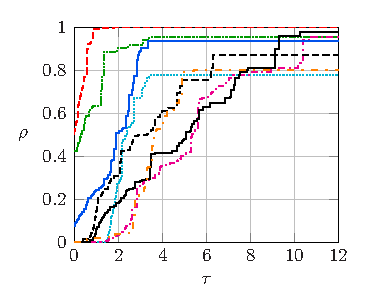
\includegraphics{lexample_fig1}
%     \caption{Example figure using external image files.}
%     \label{fig:testfig}
%   \end{figure}
%   \Cref{tab:foo} shows additional
%   supporting evidence.
% }
% \textcolor{gray}{
%   \begin{table}[htbp]
%     \footnotesize
%     \caption{Example table.}\label{tab:foo}
%     \begin{center}
%       \begin{tabular}{|c|c|c|} \hline
%         Species & \bf Mean & \bf Std.~Dev. \\ \hline
%         1       & 3.4      & 1.2           \\
%         2       & 5.4      & 0.6           \\
%         3       & 7.4      & 2.4           \\
%         4       & 9.4      & 1.8           \\ \hline
%       \end{tabular}
%     \end{center}
%   \end{table}
% }

% \section{Discussion of \texorpdfstring{{\boldmath$Z=X \cup Y$}}{Z = X union Y}}


\section{Remarks}
\label{sec:remarks}

some remarks.

In \cref{thm:regularity}
If \(f\in L^\infty(\Omega)\)  then \(u \in C_{\alpha/2}(\Omega)\), which is Proposition 1.1 in \cite{ROSOTON2014275}.

When \(\|f\|_{\beta}^{(\gamma)} < \infty\), where \(\beta > 2-\alpha\) and \(\gamma \in [-\alpha, -\alpha/2]\), we observed convergent order \(\min\{r(\alpha+\gamma), 2\}\) in numerical experiments. 
And we can prove that kind theorems with the techneque we used in this paper. 
















\appendix

\section{Approximate of difference quotients}

\begin{lemma} \label{lmm:Dh2simd2}
  If \(g(x)\in C^2\Omega\),
  there exists \(\xi \in [x_{i-1}, x_{i+1}]\) such that
  \begin{equation} \label{eq:Dh2simd2}
    \begin{aligned}
      D_h^2 g(x_i) & := \frac{2}{h_i + h_{i+1}} \left( \frac{1}{h_{i+1}} g(x_{i+1}) - (\frac{1}{h_{i}}+\frac{1}{h_{i+1}})g(x_{i}) + \frac{1}{h_{i}} g(x_{i-1}) \right) \\
      % &= \frac{h_i}{h_i + h_{i+1}} g''(\xi_1) + \frac{h_{i+1}}{h_i + h_{i+1}} g''(\xi_2)  \\
                   & = g''(\xi), \quad \xi \in [x_{i-1}, x_{i+1}]
    \end{aligned}
  \end{equation}
  \begin{equation} \label{eq:Dh2Cauchy2}
    \begin{aligned}
       & \frac{2}{h_i + h_{i+1}} \left( \frac{1}{h_{i+1}} g(x_{i+1}) - (\frac{1}{h_{i}}+\frac{1}{h_{i+1}})g(x_{i}) + \frac{1}{h_{i}} g(x_{i-1}) \right)                          \\
      % &= \frac{h_i}{h_i + h_{i+1}} g''(\xi_1) + \frac{h_{i+1}}{h_i + h_{i+1}} g''(\xi_2)  \\
       & \quad = \frac{2}{h_i + h_{i+1}} \left( \frac{1}{h_{i}}\int_{x_{i-1}}^{x_i} g''(y) (y-x_{i-1}) dy + \frac{1}{h_{i+1}} \int_{x_i}^{x_{i+1}} g''(y) (x_{i+1}-y) dy \right)
    \end{aligned}
  \end{equation}
  And if \(g(x) \in C^4(\Omega)\), then
  \begin{equation} \label{eq:Dh2simd4}
    \begin{aligned}
      \frac{2}{h_i + h_{i+1}} & \left( \frac{1}{h_{i+1}} g(x_{i+1}) - (\frac{1}{h_{i}}+\frac{1}{h_{i+1}})g(x_{i}) + \frac{1}{h_{i}} g(x_{i-1}) \right)                   \\
                              & = g''(x_{i}) + \frac{h_{i+1}-h_{i}}{3} g'''(x_{i}) + \frac{1}{4!} \frac{2}{h_i + h_{i+1}}(h_i^3 g''''(\eta_1) + h_{i+1}^3 g''''(\eta_2))
    \end{aligned}
  \end{equation}
  where \(\eta_1 \in [x_{i-1}, x_{i}], \eta_2 \in [x_{i}, x_{i+1}]\).
\end{lemma}
\begin{proof}
  \begin{gather*}
    g(x_{i-1}) = g(x_{i}) - (x_{i}-x_{i-1}) g'(x_{i}) + \frac{(x_{i}-x_{i-1})^2}{2} g''(\xi_1), \quad \xi_1 \in [x_{i-1}, x_{i}]        \\
    g(x_{i+1}) = g(x_{i}) + (x_{i+1}-x_{i}) g'(x_{i}) + \frac{(x_{i+1}-x_{i})^2}{2} g''(\xi_2), \quad \xi_2 \in [x_{i}, x_{i+1}]
  \end{gather*}
  Subsitute them in the left side of \eqref{eq:Dh2simd2}, we have
  \begin{equation*}
    \begin{aligned}
      \frac{2}{h_i + h_{i+1}} & \left( \frac{1}{h_{i+1}} g(x_{i+1}) - (\frac{1}{h_{i}}+\frac{1}{h_{i+1}})g(x_{i}) + \frac{1}{h_{i}} g(x_{i-1}) \right) \\
                              & = \frac{h_i}{h_i + h_{i+1}} g''(\xi_1) + \frac{h_{i+1}}{h_i + h_{i+1}} g''(\xi_2)
    \end{aligned}
  \end{equation*}
  Now, using \textcolor{red}{intermediate value theorem} , there exists \(\xi \in [\xi_1, \xi_2]\) such that
  \begin{equation*}
    \frac{h_i}{h_i + h_{i+1}} g''(\xi_1) + \frac{h_{i+1}}{h_i + h_{i+1}} g''(\xi_2) = g''(\xi)
  \end{equation*}
  For the second equation, similarly
  \begin{gather*}
    g(x_{i-1}) = g(x_{i}) - (x_{i}-x_{i-1}) g'(x_{i}) + \int_{x_{i-1}}^{x_i} g''(y) (y-x_{i-1}) dy \\
    g(x_{i+1}) = g(x_{i}) + (x_{i+1}-x_{i}) g'(x_{i}) + \int_{x_i}^{x_{i+1}} g''(y) (x_{i+1}-y) dy
  \end{gather*}
  And the last equation can be obtained by
  \begin{gather*}
    g(x_{i-1}) = g(x_{i}) - h_{i} g'(x_{i}) + \frac{h_{i}^2}{2} g''(x_{i}) - \frac{h_{i}^3}{3!} g'''(x_{i}) +  \int_{x_{i-1}}^{x_{i}} g''''(y) \frac{(y-x_{i-1})^3}{3!} dy        \\
    g(x_{i+1}) = g(x_{i}) + h_{i+1} g'(x_{i}) + \frac{h_{i+1}^2}{2} g''(x_{i}) + \frac{h_{i+1}^3}{3!} g'''(x_{i}) + \int_{x_{i}}^{x_{i+1}} g''''(y) \frac{(x_{i+1}-y)^3}{3!} dy
  \end{gather*}
  Expecially,
  \begin{equation} \label{eq:Dh2Cauchy4}
    \begin{aligned}
      \int_{x_{i-1}}^{x_{i}} g''''(y) \frac{(y-x_{i-1})^3}{3!} dy & = \frac{h_i^4}{4!}g''''(\eta_1) \\
      \int_{x_{i}}^{x_{i+1}} g''''(y) \frac{(x_{i+1}-y)^3}{3!} dy & = \frac{h_{i+1}^4}{4!}g''''(\eta_2)
    \end{aligned}
  \end{equation}
  where \(\eta_1 \in [x_{i-1}, x_{i}], \eta_2 \in [x_{i}, x_{i+1}]\).
  Subsitute them to the left side of \eqref{eq:Dh2simd4}, we can get the result.
\end{proof}


\begin{lemma} \label{lmm:Dyj}
  Denote \(y_j^\theta = \theta x_{j-1} + (1-\theta) x_j, \theta\in [0,1]\),
  % then for \(2\le j \le 2N-1\)
  \begin{equation}
    \begin{aligned}
      u(y_j^\theta) - u_h(y_j^\theta) & = -\frac{\theta (1-\theta)}{2} h_j^2 u''(\xi), \quad \xi \in [x_{j-1}, x_j]
    \end{aligned}
  \end{equation}
  \begin{equation}
    \begin{aligned}
      u(y_j^\theta) - u_h(y_j^\theta) = & -\frac{\theta (1-\theta)}{2} h_j^2 u''(y_j^\theta)
      + \frac{\theta (1-\theta)}{3!} h_j^3 ((1-\theta)^2 u'''(\eta_1) - \theta^2 u'''(\eta_2))
    \end{aligned}
  \end{equation}
  where \(\eta_1 \in [x_{j-1}, y_j^\theta], \eta_2 \in [y_j^\theta, x_j]\).
\end{lemma}
\begin{proof}
  By Taylor expansion, we have
  \begin{gather*}
    u(x_{j-1}) = u(y_j^\theta) - (1-\theta) h_{j} u'(y_j^\theta) + \frac{(1-\theta)^2 h_{j}^2}{2!} u''(\xi_1), \quad \xi_1 \in [x_{j-1}, y_j^\theta] \\
    u(x_{j}) = u(y_j^\theta) + \theta h_{j} u'(y_j^\theta) + \frac{\theta^2 h_{j}^2}{2!} u''(\xi_2) , \quad \xi_2 \in [y_j^\theta, x_j]
  \end{gather*}
  Thus
  \begin{equation*}
    \begin{aligned}
      u(y_j^\theta) - u_h(y_j^\theta) & = u(y_j^\theta) - \theta u(x_{j-1}) - (1-\theta)u(x_{j})                          \\
                                      & = -\frac{\theta (1-\theta)}{2} h_j^2 ((1-\theta)u''(\xi_1) +  \theta u''(\xi_2) ) \\
                                      & = -\frac{\theta (1-\theta)}{2} h_j^2 u''(\xi), \quad \xi \in [\xi_1, \xi_2]
    \end{aligned}
  \end{equation*}
  The second equation is similar,
  \begin{gather*}
    u(x_{j-1}) = u(y_j^\theta) - (1-\theta)h_{j} u'(y_j^\theta) + \frac{ (1-\theta)^2h_{j}^2}{2!} u''(y_j^\theta) - \frac{(1-\theta)^3 h_{j}^3}{3!} u'''(\eta_1)  \\
    u(x_{j}) = u(y_j^\theta) +  \theta h_{j} u'(y_j^\theta) + \frac{\theta^2 h_{j}^2}{2!} u''(y_j^\theta) + \frac{\theta^3 h_{j}^3}{3!} u'''(\eta_2)
  \end{gather*}
  where \(\eta_1 \in [x_{j-1}, y_j^\theta], \eta_2 \in [y_j^\theta, x_j]\).
  Thus
  \begin{equation*}
    \begin{aligned}
      u(y_j^\theta) - u_h(y_j^\theta) & = u(y_j^\theta) - \theta u(x_{j-1}) - (1-\theta)u(x_{j})   \\
                                      & = -\frac{\theta (1-\theta)}{2} h_j^2 u''(y_j^\theta) + \frac{\theta (1-\theta)}{3!} h_j^3 ( (1-\theta)^2 u'''(\eta_1) - \theta^2 u'''(\eta_2))
    \end{aligned}
  \end{equation*}
\end{proof}

\begin{lemma} \label{lmm:Dyj1}
  For \(x\in [x_{j-1}, x_j]\)
  \begin{equation}
    \begin{aligned}
      |u(x) - u_h(x)| & = \left| \frac{x_{j}-x}{h_j} \int_{x_{j-1}}^x u'(y) dy - \frac{x-x_{j-1}}{h_j} \int_{x}^{x_{j}} u'(y) dy \right| \\
                      & \le \int_{x_{j-1}}^{x_{j}} |u'(y)| dy
    \end{aligned}
  \end{equation}
  If \(x\in [0, x_1]\), with \cref{cor:regularity-u}, we have
  \begin{equation}
    |u(x) - u_h(x)| \le \int_{0}^{x_1} |u'(y)| dy \le \int_{0}^{x_1} C y^{\alpha/2-1} dy  \le C\frac{2}{\alpha} x_1^{\alpha/2}
  \end{equation}
  Similarly, if \(x\in [x_{2N-1}, 1]\), we have
  \begin{equation}
    |u(x) - u_h(x)| \le C\frac{2}{\alpha} (2T-x_{2N-1})^{\alpha/2} = C\frac{2}{\alpha} x_1^{\alpha/2}
  \end{equation}
\end{lemma}


\section{Inequality}

\textcolor{blue}{
  \begin{lemma} \label{lmm:hilexi}
    \begin{equation}
      h_i \le r T^{1/r} h \begin{cases}
        x_i^{1-1/r},          & 1\le i \le N   \\
        (2T-x_{i-1})^{1-1/r}, & N < i \le 2N-1
      \end{cases}
    \end{equation}
    \begin{equation}
      h_i \ge r T^{1/r} h \begin{cases}
        x_{i-1}^{1-1/r},    & 1\le i \le N   \\
        (2T-x_{i})^{1-1/r}, & N < i \le 2N-1
      \end{cases}
    \end{equation}
  \end{lemma}
  \begin{proof}
    For \(1\le i \le N\),
    \begin{displaymath}
      \begin{aligned}
        h_i & = T \left( \left(\frac{i}{N}\right)^r - \left(\frac{i-1}{N}\right)^r \right)  \\
            & \le rT \frac{1}{N} \left(\frac{i}{N}\right)^{r-1} = r T^{1/r} h x_{i}^{1-1/r} \\
      \end{aligned}
    \end{displaymath}
    \begin{displaymath}
      h_i \ge r T \frac{1}{N} \left(\frac{i-1}{N}\right)^{r-1} = r T^{1/r} h x_{i-1}^{1-1/r}
    \end{displaymath}
    For \(N < i \le 2N\),
    \begin{displaymath}
      \begin{aligned}
        h_i & = T\left(  \left(\frac{2N-i+1}{N}\right)^r - \left(\frac{2N-i}{N}\right)^r \right)        \\
            & \le rT \frac{1}{N} \left(\frac{2N-i+1}{N}\right)^{r-1} = r T^{1/r} h (2T-x_{i-1})^{1-1/r} \\
      \end{aligned}
    \end{displaymath}
    \begin{displaymath}
      h_i \ge r T \frac{1}{N} \left(\frac{2N-i}{N}\right)^{r-1} = r T^{1/r} h (2T-x_{i})^{1-1/r}
    \end{displaymath}
  \end{proof}
}


\textcolor{blue}{
  \begin{lemma} \label{lmm:hi1-hi}
    There is a constant \(C=2^{|r-2|}r(r-1)T^{2/r}\) such that for all \(i\in\{1,2,\cdots,2N-1\}\)
    \begin{equation}
      |h_{i+1} - h_{i}| \le C h^2 \begin{cases}
        x_i^{1-2/r} ,     & 1\le i\le N-1 \\
        0,                & i=N           \\
        (2T-x_i)^{1-2/r}, & N<i\le 2N-1   \\
      \end{cases}
    \end{equation}
  \end{lemma}
  \begin{proof}
    \begin{equation*}
      \begin{aligned}
        h_{i+1} - h_{i} =
        \begin{cases}
          T \left( \left(\frac{i+1}{N}\right)^r - 2\left(\frac{i}{N}\right)^r + \left(\frac{i-1}{N}\right)^r  \right) ,           & 1\le i\le N-1    \\
          0,                                                                                                                      & i=N              \\
          -T \left( \left(\frac{2N-i-1}{N}\right)^r - 2\left(\frac{2N-i}{N}\right)^r + \left(\frac{2N-i+1}{N}\right)^r  \right) , & N+1\le i\le 2N-1 \\
        \end{cases}
      \end{aligned}
    \end{equation*}
    % if \(r=2\), 
    % \begin{equation*}
    %   h_{i+1}-h_{i} = 2T N^{-2}, \quad 1-2/r=0
    % \end{equation*}
    For \(i=1\),
    \begin{equation*}
      \begin{aligned}
        h_2-h_1 & = T(2^{r}-2)\left(\frac{1}{N}\right)^r = (2^{r}-2)T^{2/r} h^2 x_1^{1-2/r}
      \end{aligned}
    \end{equation*}
    For \(2\le i\le N-1\), by \cref{lmm:Dh2simd2}, we have
    \begin{equation*}
      \begin{aligned}
        h_{i+1} - h_{i} & =  r(r-1) T \; N^{-2} \eta^{r-2}, \quad \eta \in [\frac{i-1}{N}, \frac{i+1}{N}]  \\
        &= C (r-1) h^2 x_i^{1-2/r}
      \end{aligned}
    \end{equation*}
    % If \(r\in[1, 2]\),
    % \begin{equation*}
    %   \begin{aligned}
    %     h_{i+1} - h_{i} & =  r(r-1) T \; N^{-2} \eta^{r-2}
    %     \le r(r-1) T \; h^2 \left( \frac{i-1}{N} \right)^{r-2}                         \\
    %                     & \le r(r-1) T \; h^2 2^{2-r} \left( \frac{i}{N} \right)^{r-2} \\
    %                     & = 2^{2-r} r(r-1) T^{2/r} h^2 x_i^{1-2/r}
    %   \end{aligned}
    % \end{equation*}
    % else if \(r>2\),
    % \begin{equation*}
    %   \begin{aligned}
    %     h_{i+1} - h_{i} & =  r(r-1) T \; N^{-2} \eta^{r-2}
    %     \le r(r-1) T \; h^2 \left( \frac{i+1}{N} \right)^{r-2}                         \\
    %                     & \le r(r-1) T \; h^2 2^{r-2} \left( \frac{i}{N} \right)^{r-2} \\
    %                     & = 2^{r-2} r(r-1) T^{2/r} h^2 x_i^{1-2/r}
    %   \end{aligned}
    % \end{equation*}
    % Since
    % \begin{equation*}
    %   2^r-2 \le 2^{|r-2|}r(r-1), \quad r\ge 1
    % \end{equation*}
    % we have
    % \begin{equation*}
    %   h_{i+1} - h_{i} \le 2^{|r-2|}r(r-1)T^{2/r} h^2 x_i^{1-2/r},  \quad 1\le i\le N-1
    % \end{equation*}
    % For \(i=N\), \( h_{N+1}-h_{N} = 0\).
    % For \(N<i\le 2N-1\), it's central symmetric to the first half of the proof, which is
    % % \begin{equation*}
    % %   \begin{aligned}
    % %     h_{2N-1} - h_{2N} & =
    % %       T(2^{r}-2)\left(\frac{1}{N}\right)^r = (2^{r}-2)T^{2/r} h^2 (2T-x_{2N-1})^{1-2/r}
    % %   \end{aligned}
    % % \end{equation*}
    % % and
    % \begin{equation*}
    %   h_{i}-h_{i+1} \le 2^{|r-2|}r(r-1)T^{2/r} h^2 (2T-x_{i})^{1-2/r}
    % \end{equation*}
    Summarizes the inequalities, we can get
    \begin{equation}
      |h_{i+1} - h_{i}| \le 2^{|r-2|}r(r-1)T^{2/r} h^2 \begin{cases}
        x_i^{1-2/r} ,     & 1\le i\le N-1 \\
        0,                & i=N           \\
        (2T-x_i)^{1-2/r}, & N<i\le 2N-1
      \end{cases}
    \end{equation}
  \end{proof}
}




\section{Proofs of some technical details}

\begin{proof}[Additional proof of \cref{lmm:trunerror2}] \label{prf:trucerr2d2f}
  For \(2\le i \le N-1\),
  \begin{equation*}
    \begin{aligned}
      \frac{2}{h_i + h_{i+1}} & (h_i^3 f''(\eta_1) + h_{i+1}^3 f''(\eta_2))                                                \\
                              & \le C\frac{2}{h_i + h_{i+1}} (h_i^3 x_{i-1}^{-2-\alpha/2} + h_{i+1}^3 x_{i}^{-2-\alpha/2}) \\
                              & \le 2C (h_i^2 x_{i-1}^{-2-\alpha/2} + h_{i+1}^2 x_{i}^{-2-\alpha/2})
    \end{aligned}
  \end{equation*}
  % Since \cref{lmm:hilexi}, we have
  % \begin{gather*}
  %   h_i \le r T^{1/r} h x_{i}^{1-1/r}, \quad 1\le i\le N \\
  %   h_{i+1} \le r T^{1/r} h x_{i+1}^{1-1/r}, \quad 1\le i\le N-1
  % \end{gather*}
  % and
  % \begin{gather*}
  %   x_{i-1}^{-2-\alpha/2} \le 2^{-r(-2-\alpha/2)} x_i^{-2-\alpha/2}  \quad 2\le i\le N-1 \\
  %   x_{i+1}^{1-1/r} \le 2^{r-1} x_i^{1-1/r} \quad 1\le i \le N-1
  % \end{gather*}
  There is a constant \(C=C(T, \alpha, r, \|f\|_{\beta}^{\alpha/2})\) such that
  \begin{equation*}
    \frac{2}{h_i + h_{i+1}} (h_i^3 f''(\eta_1) + h_{i+1}^3 f''(\eta_2)) \le C h^2 x_i^{-\alpha/2-2/r}, \quad 2\le i\le N-1
  \end{equation*}
  For \(i=1\), by \eqref{eq:Dh2Cauchy4}
  \begin{equation*}
    \begin{aligned}
       & \frac{1}{4!}\frac{2}{h_1 + h_{2}} (h_1^3 f''(\eta_1) + h_{2}^3 f''(\eta_2))                  \\
       & \quad =  \frac{2}{h_1 + h_{2}} \left( \frac{1}{h_1}\int_{0}^{x_1} f''(y) \frac{y^3}{3!} dy +
      \frac{1}{4!} h_2^3 f''(\eta_2) \right)                                                          \\
    \end{aligned}
  \end{equation*}
  We have proved above that
  \begin{equation*}
    \frac{2}{h_1 + h_{2}} h_2^3 f''(\eta_2) \le C h^2 x_1^{-\alpha/2-2/r}
  \end{equation*}
  and we can get
  \begin{equation*}
    \begin{aligned}
      \int_{0}^{x_1} f''(y) \frac{y^3}{3!} dy & \le C \frac{1}{3!}\int_{0}^{x_1} y^{1-\alpha/2} dy \\
                                              & = C\frac{1}{3!(2-\alpha/2)} x_1^{2-\alpha/2}       \\
    \end{aligned}
  \end{equation*}
  so
  \begin{equation*}
    \frac{2}{h_1 + h_{2}} \frac{1}{h_1}\int_{0}^{x_1} f''(y) \frac{y^3}{3!} dy = \frac{C 2^{1-r}}{3!(2-\alpha/2)}x_1^{-\alpha/2} = \frac{C 2^{1-r}}{3!(2-\alpha/2)} T^{2/r} h^2 x_1^{-\alpha/2-2/r}
  \end{equation*}
  And for \(i=N\), we have
  \begin{equation*}
    \begin{aligned}
      \frac{2}{h_N + h_{N+1}} & (h_N^3 f''(\eta_1) + h_{N+1}^3 f''(\eta_2))                       \\
                              & = h_N^{2} (f''(\eta_1) + f''(\eta_2))                             \\
                              & \le r^2 T^{2/r} h^2 x_N^{2-2/r} \; 2C x_{N-1}^{-2-\alpha/2}       \\
                              & \le 2 r^2 T^{2/r} C 2^{-r(-2-\alpha/2)}\; h^2 x_N^{-\alpha/2-2/r} \\
    \end{aligned}
  \end{equation*}
  Finally, \(N+1 \le i \le 2N-1\) is symmetric to the first half of the proof, so we can conclude that
  \begin{equation*}
    \frac{2}{h_i + h_{i+1}} (h_i^3 f''(\eta_1) + h_{i+1}^3 f''(\eta_2)) \le C h^2
    \begin{cases}
      x_i^{-\alpha/2-2/r}, & 1\le i\le N \\ (2T-x_i)^{-\alpha/2-2/r}, & N\le i\le 2N-1
    \end{cases}
  \end{equation*}
\end{proof}

\begin{lemma} \label{lmm:Dyjleh2ya/2m2/r}
  By a standard error estimate for linear interpolation, and \cref{cor:regularity-u},
  There is a constant \(C=C(T, \alpha, r, \|u\|_{\beta+\alpha}^{(-\alpha/2)})\) for \(2\le j \le N\),
  \begin{equation}
    |u(y)-u_h(y)| \le C h^2 y^{\alpha/2-2/r}, \quad \text{for } y\in [x_{j-1}, x_{j}]
  \end{equation}
  symmetricly, for \(N <j \le 2N-1\), we have
  \begin{equation} \label{lmm:Dyjleh22T-y}
    |u(y) - u_h(y)| \le C h^2 (2T-y)^{\alpha/2-2/r}
  \end{equation}
\end{lemma}
% \begin{proof}
%   For  \(2\le j \le N\),  we have
%   \begin{equation*}
%     x_j \le 2^r y, \quad x_{j-1} \ge 2^{-r} y
%   \end{equation*}
%   And by \cref{lmm:Dyj}, \cref{lmm:hilexi} and \cref{cor:regularity-u}, we have
%   \begin{equation*}
%     \begin{aligned}
%       u(y)-u_h(y) & = -\frac{\theta (1-\theta)}{2} h_j^2 u''(\xi), \quad \xi \in [x_{j-1}, x_j]                         \\
%                   & \le \frac{\|u\|_{\beta+\alpha}^{(-\alpha/2)}}{4} r^2T^{2/r} \; h^2 x_j^{2-2/r} x_{j-1}^{\alpha/2-2} \\
%                   & \le C h^2 \; 2^{2r-2} y^{2-2/r} \; 2^{-r(\alpha/2-2)} y^{\alpha/2-2}                                \\
%                   & = C 2^{-r\alpha/2+4r-2} \; h^2 y^{\alpha/2-2/r}
%     \end{aligned}
%   \end{equation*}
%   

% \end{proof}


\begin{lemma} \label{lmm:Dh2ymx1malecy1ma}
  There is a constant \(C=C(\alpha, r)\) such that for all \(1 \le i < N/2\), \\
  \(\max\{2i+1, i+3\} \le j \le 2N\) , we have
  \begin{equation}
    D_h^2 K_y (x_i) \le C \frac{y^{-1-\alpha}}{\Gamma(-\alpha)}, \quad y\in [x_{j-1}, x_{j}]
  \end{equation}
\end{lemma}
\begin{proof}
  Sinec \(y\ge x_{j-1} > x_{i+1}\), by \cref{lmm:Dh2simd2}, if \(j-1>i+1\)
  \begin{equation*}
    \begin{aligned}
      D_h^2 K_y (x_i) & = K_y''(\xi)= \frac{|y-\xi|^{-1-\alpha}}{\Gamma(-\alpha)}, \quad \xi \in [x_{i-1}, x_{i+1}] \\
                      & \le \frac{(y-x_{i+1})^{-1-\alpha}}{\Gamma(-\alpha)}                             \\
                      & \le (1-(\frac{2}{3})^r)^{-1-\alpha}\frac{y^{-1-\alpha}}{\Gamma(-\alpha)}
    \end{aligned}
  \end{equation*}
\end{proof}


\begin{lemma} \label{lmm:Dh2xmy1malecx1ma}
  There is a constant \(C=C(\alpha, r)\) such that for all \(3 \le i \le N, k = \lceil \frac{i}{2} \rceil\),
  \(1 \le j \le k-1\) and \(y\in [x_{j-1}, x_{j}]\), we have
  \begin{equation}
    D_h^2 K_y (x_i) \le C \frac{x_i^{-1-\alpha}}{\Gamma(-\alpha)}
  \end{equation}
\end{lemma}
\begin{proof}
  Sinec \(y \le x_{j} < x_{i-1}\), by \cref{lmm:Dh2simd2},
  \begin{equation*}
    \begin{aligned}
      D_h^2 K_y (x_i) & = \frac{|\xi-y|^{-1-\alpha}}{\Gamma(-\alpha)}, \quad \xi \in [x_{i-1}, x_{i+1}]                                    \\
                                                                & \le \frac{(x_{i-1}-x_{j})^{-1-\alpha}}{\Gamma(-\alpha)}  \le \frac{(x_{i-1}-x_{k-1})^{-1-\alpha}}{\Gamma(-\alpha)} \\
                                                                & \le ((\frac{2}{3})^r-(\frac{1}{2})^r)^{-1-\alpha}\frac{x_i^{-1-\alpha}}{\Gamma(-\alpha)}
    \end{aligned}
  \end{equation*}
\end{proof}

\textcolor{brown}{
  \begin{lemma} \label{lmm:Ti1}
    While \(0 \le i < N/2\),
    By \cref{lmm:Dyj1}
    \begin{equation}
      \begin{aligned}
        |T_{i1}| & \le C \int_{0}^{x_1} x_1^{\alpha/2} \frac{|x_i-y|^{1-\alpha}}{\Gamma(2-\alpha)} dy                                             \\
                 & = C \frac{1}{\Gamma(3-\alpha)} x_1^{\alpha/2}  \left| x_i^{2-\alpha} - |x_i-x_1|^{2-\alpha} \right|                            \\
                 & \le C \frac{1}{\Gamma(3-\alpha)} x_1^{\alpha/2 + 2-\alpha} =  C \frac{1}{\Gamma(3-\alpha)} x_1^{2-\alpha/2} \quad 0<2-\alpha<1
      \end{aligned}
    \end{equation}
    For \(2\le j \le N\), by \cref{lmm:Dyj} and \cref{cor:regularity-u}
    \begin{equation}
      \begin{aligned}
        |T_{ij}| & \le \frac{C}{4} \int_{x_{j-1}}^{x_j} h_j^2 x_{j-1}^{\alpha/2-2}  \frac{|y-x_i|^{1-\alpha}}{\Gamma(2-\alpha)} dy                \\
                 & \le \frac{C}{4 \Gamma(3-\alpha)}  h_j^2 x_{j-1}^{\alpha/2-2}  \left| |x_j-x_i|^{2-\alpha} - |x_{j-1}-x_{i}|^{2-\alpha} \right| \\
      \end{aligned}
    \end{equation}
  \end{lemma}
}


\begin{lemma} \label{lmm:sumSij13}
  There exists a constant \(C=C(T, \alpha, r, \|u\|_{\beta+\alpha}^{(-\alpha/2)})\) such that
  \begin{equation}
    \sum_{j=1}^{3} S_{1j} \le C h^2 x_1^{-\alpha/2-2/r}
  \end{equation}
  \textcolor{orange}{
    \begin{equation}
      \sum_{j=1}^{4} S_{2j} \le C h^2 x_2^{-\alpha/2-2/r}
    \end{equation}
  }
\end{lemma}
\begin{proof}
  \begin{equation*}
    \begin{aligned}
      S_{1j} = \frac{2}{x_2}\left( \frac{1}{x_1}T_{0j} - \left(\frac{1}{x_1} + \frac{1}{h_2}\right) T_{1j} + \frac{1}{h_2} T_{2j} \right) \\
    \end{aligned}
  \end{equation*}
  So, by \cref{lmm:Ti1}
  \begin{equation*}
    S_{11} \le \frac{2}{x_2 x_1} 4 \frac{C}{\Gamma(3-\alpha)} x_1^{2-\alpha/2} \le C x_1^{-\alpha/2}
  \end{equation*}
  \begin{equation*}
    \begin{aligned}
      S_{12} & \le  \frac{2}{x_2 x_1} \frac{C}{4\Gamma(3-\alpha)} h_2^2 x_{1}^{\alpha/2-2}
      \left(  x_2^{2-\alpha} + 2 h_2^{2-\alpha} + h_2^{2-\alpha}    \right)
      \le C x_1^{-\alpha/2}
    \end{aligned}
  \end{equation*}
  \begin{equation*}
    \begin{aligned}
      S_{13} & \le  \frac{2}{x_2 x_1} \frac{C}{4\Gamma(3-\alpha)} h_3^2 x_{2}^{\alpha/2-2}
      \left(  x_3^{2-\alpha} + 2 x_3^{2-\alpha} + h_3^{2-\alpha}    \right)
      \le C x_1^{-\alpha/2}
    \end{aligned}
  \end{equation*}
  But
  \begin{equation*}
    x_1^{-\alpha/2} = T^{2/r} h^2 x_1^{-\alpha/2-2/r}
  \end{equation*}
  \(i=2\) is similar.
\end{proof}


\textcolor{orange}{
  \begin{lemma} \label{lmm:dhj-i3le-Ch2xi1-2r}
    There exists a constant \(C=C(T, r, l)\) such that
    For \(3\le i \le N-1, k+1=\lceil\frac{i}{2}\rceil, k \le j \le \min\{2i-1, N-1\}\),
    \(l=3, 4\), \\
    when \(\xi \in [x_{i-1}, x_{i+1}]\),
    \begin{equation}
      (h_{j-i}^3(\xi))' \le (r-1) C h^2  x_{i}^{1-2/r} h_{j}
    \end{equation}
    \begin{equation}
      (h_{j-i}^4(\xi))' \le (r-1) C h^2 x_{i}^{1-2/r} h_{j}^2
    \end{equation}
  \end{lemma}
}
\begin{proof}
  From \eqref{def:xi2yj-jlN}
  \begin{gather} \label{eq:yj-i-diff}
    y_{j-i}'(x) = y_{j-i}^{1-1/r}(x) x^{1/r-1}  \\
    y_{j-i}''(x) = \frac{1-r}{r} y_{j-i}^{1-2/r}(x) x^{1/r-2} Z_{j-i}
  \end{gather}
  for \(l=3, 4\), by \eqref{def:hj-jlN}
  \begin{equation}
    \begin{aligned}
      (h_{j-i}^l(\xi))' & = l \; h_{j-i}^{l-1}(\xi)(y_{j-i}'(\xi)-y_{j-i-1}'(\xi))                                   \\
                        & = l \; h_{j-i}^{l-1}(\xi) \xi^{1/r-1} (y_{j-i}^{1-1/r}(\xi)- y_{j-i-1}^{1-1/r}(\xi)) \ge 0 \\
    \end{aligned}
  \end{equation}
  For \(\xi\in [x_{i-1}, x_{i+1}]\) and \(2\le k \le j \le \min\{2i-1, N-1\}\), using \cref{lmm:hilexi}
  \begin{equation*}
    \begin{aligned}
      h_{j-i}(\xi) & \le h_{j-i}(x_{i+1}) = h_{j+1}                                          \\
                   & \le rT^{1/r} \; h x_{j+1}^{1-1/r} \le rT^{1/r}2^{r-1} \; hx_{i}^{1-1/r} \\
    \end{aligned}
  \end{equation*}
  And
  \begin{equation}
    2^{-r}x_i  \le x_{i-1} \le \xi \le x_{i+1} \le 2^r x_i
  \end{equation}
  We have
  \begin{equation}
    \xi^{1/r-m} \le 2^{|mr-1|} x_i^{1/r-m}, \quad m=1,2
  \end{equation}
  but
  \begin{equation}
    \begin{aligned}
      y_{j-i}^{1-1/r}(\xi)- y_{j-i-1}^{1-1/r}(\xi) & = (\xi^{1/r}+ Z_{j-i})^{r-1} - (\xi^{1/r}+ Z_{j-i-1})^{r-1}           \\
                                                   & = (r-1)Z_{1} (\xi^{1/r}+ Z_{j-i-\gamma})^{r-2}, \quad \gamma\in [0,1] \\
                                                   & = (r-1)T^{1/r} h y_{j-i-\gamma}^{1-2/r}(\xi)
    \end{aligned}
  \end{equation}
  And
  \begin{equation} \label{eq:xj-2-xjp1-xi}
    4^{-r} x_i \le x_{\lceil\frac{i}{2}\rceil-1} \le x_{j-2} = y_{j-i-1}(x_{i-1}) \le  y_{j-i-\gamma}(\xi) \le y_{j-i}(x_{i+1}) = x_{j+1} \le x_{2i} \le 2^r x_{i} \\
  \end{equation}
  Therefore,
  \begin{equation}
    y_{j-i-\gamma}^{1-2/r}(\xi) \le 2^{2|r-2|} x_i^{1-2/r}
  \end{equation}
  So we can get
  \begin{equation} \label{eq:yj1-1/r-yj-1}
    y_{j-i}'(\xi)- y_{j-i-1}'(\xi) \le (r-1) C(T,r) h x_i^{-1/r}
  \end{equation}

  We get
  \begin{equation}
    (h_{j-i}^l(\xi))' \le l(r-1) C \; h_{j+1}^{l-1}  h  x_i^{-1/r}  \\
  \end{equation}
  And by \cref{lmm:hilexi},
  \begin{equation}
    h_{j+1} \le rT h \left(\frac{j+1}{N}\right)^{r-1} \le rTh 2^{r-1} \left(\frac{j-1}{N}\right) = 2^{r-1} h_{j}
  \end{equation}
  \begin{equation}
    h_{j+1} \le rT^{1/r} h x_{j+1}^{1-1/r} \le rT^{1/r} h x_{2i}^{1-1/r} \le rT^{1/r}2^{r-1} h x_{i}^{1-1/r}
  \end{equation}
  % \begin{equation}
  %   x_{i+1}^{1/r-1} \le (\frac{4}{3})^{1/r-1} x_{i}^{1/r-1}
  % \end{equation}
  We can get
  \begin{equation}
    \begin{aligned}
      (h_{j-i}^l(\xi))' & \le l(r-1)C \; h_j^{l-2}  h_{j+1}  h  x_i^{-1/r}        \\
                        & \le l (r-1)C h h_j^{l-2} ( h x_{i}^{1-1/r})  x_i^{-1/r} \\
                        & = (r-1)C \; h^2   x_i^{1-2/r} h_j^{l-2}
    \end{aligned}
  \end{equation}
  Meanwhile, we can get
  \begin{gather} \label{eq:hj-i3leCh2x2-2rhj}
    h_{j-i}^3(\xi) \le h_{j+1}^3 \le C h^{2} x_{i}^{2-2/r}  h_j \\
    h_{j-i}^4(\xi) \le h_{j+1}^4 \le C h^{2} x_{i}^{2-2/r}  h_j^2
  \end{gather}
\end{proof}


\textcolor{orange}{
  \begin{lemma} \label{lmm:d2hj-i3leh2xi-2r}
    There exists a constant \(C=C(T, r, l)\) such that
    For \(3\le i \le N-1, \lceil\frac{i}{2}\rceil+1 \le j \le \min\{2i-1, N-1\}\), \\
    when \(\xi \in [x_{i-1}, x_{i+1}]\),
    \begin{equation}
      (h_{j-i}^3(\xi))'' \le C(r-1)  h^2  x_{i}^{-2/r} h_{j}
    \end{equation}
  \end{lemma}
}
\begin{proof}
  From \eqref{eq:yj-i-diff}
  \begin{equation}
    \begin{aligned}
      (h_{j-i}^3(\xi))'' & = 6 h_{j-i}(\xi)(y_{j-i}'(\xi)-y_{j-i-1}'(\xi))^2 + 3 h_{j-i}^2(\xi)( y_{j-i}''(\xi)-y_{j-i-1}''(\xi))               \\
                         & = 6 h_{j-i}(\xi) (\xi^{1/r-1} (y_{j-i}^{1-1/r}(\xi)- y_{j-i-1}^{1-1/r}(\xi)))^2                                \\
                         & \quad + 3 \frac{1-r}{r} h_{j-i}^2(\xi)\xi^{1/r-2}( y_{j-i}^{1-2/r}(\xi)  Z_{j-i} - y_{j-i-1}^{1-2/r}(\xi) Z_{j-i-1}) \\
    \end{aligned}
  \end{equation}
  Using the inequalities of the proof of \cref{lmm:dhj-i3le-Ch2xi1-2r}
  \begin{equation}
    \begin{aligned}
      6 h_{j-i}(\xi) & (y_{j-i}'(\xi)-y_{j-i-1}'(\xi))^2        \\
                     & \le 6 h_{j+1} ( (r-1)C h x_{i}^{-1/r})^2 \\
                     & \le C(r-1)^2  \; h^2 x_i^{-2/r} h_j
    \end{aligned}
  \end{equation}
  For the second partial
  \begin{equation}
    \begin{aligned}
      h_{j-i}^2(\xi) & \xi^{1/r-2} ( y_{j-i}^{1-2/r}(\xi)  Z_{j-i} - y_{j-i-1}^{1-2/r}(\xi) Z_{j-i-1})                                        \\
                     & \le C h_{j+1}^2 x_{i}^{1/r-2} ( (y_{j-i}^{1-2/r}(\xi)-y_{j-i-1}^{1-2/r}(\xi)) Z_{j-i} +  y_{j-i-1}^{1-2/r}(\xi) Z_{1})
    \end{aligned}
  \end{equation}
  but
  \begin{equation}
    \begin{aligned}
      y_{j-i}^{1-2/r}(\xi)-y_{j-i-1}^{1-2/r}(\xi)
       & = (\xi^{1/r} + Z_{j-i})^{r-2} - (\xi^{1/r} + Z_{j-i-1})^{r-2} \\
       & = (r-2) Z_1 (\xi^{1/r} + Z_{j-i-\gamma})^{r-3}                \\
       & = (r-2) T^{1/r} h y_{j-i-\gamma}^{1-3/r}(\xi)                  \\
       & \le C(r-2) h x_i^{1-3/r}
    \end{aligned}
  \end{equation}
  So we can get
  \begin{equation}
    \begin{aligned}
      h_{j-i}^2(\xi) & \xi^{1/r-2} ( y_{j-i}^{1-2/r}(\xi)  Z_{j-i} - y_{j-i-1}^{1-2/r}(\xi) Z_{j-i-1})               \\
                     & \le C h_{j} h x_i^{1-1/r} x_{i}^{1/r-2} (C(r-2)hx_i^{1-3/r} Z_{j-i} + C x_i^{1-2/r} T^{1/r}h) \\
                     & \le C h^2 ((r-2) x_i^{-3/r} x_{|j-i|}^{1/r} + x_i^{-2/r}) h_j                                 \\
                     & \le C h^2 x_{i}^{-2/r} h_j
    \end{aligned}
  \end{equation}
  Summarizes, we have
  \begin{equation}
    (h_{j-i}^3(\xi))'' \le C(r-1)  h^2  x_{i}^{-2/r} h_{j}
  \end{equation}
\end{proof}

\begin{proof}[proof of \cref{lmm:estimatesofu2yj-itheta}] \label{prf:estimatesofu2yj-itheta}
  From \eqref{def:xi2yj-jlN}
  \begin{gather}
    y_{j-i}'(x) = y_{j-i}^{1-1/r}(x) x^{1/r-1}  \\
    y_{j-i}''(x) = \frac{1-r}{r} y_{j-i}^{1-2/r}(x) x^{1/r-2} Z_{j-i}
  \end{gather}
  Since
  \begin{equation*}
    x_{j-2} \le y_{j-i-1}(x_{i-1}) \le  y_{j-i}^\theta(\xi) \le y_{j-i}^\theta(x_{i+1}) \le x_{j+1}
  \end{equation*}
  We have known \eqref{eq:xj-2-xjp1-xi}
  \begin{equation}
    u''(y_{j-i}^{\theta}(\xi)) \le C ({y_{j-i}^{\theta}}(\xi))^{\alpha/2-2} \le C x_{j-2}^{\alpha/2-2} \le  C x_{\lceil\frac{i}{2}\rceil-1}^{\alpha/2-2} \le  C 4^{r(2-\alpha/2)} x_i^{\alpha/2-2}
  \end{equation}
  \begin{equation}
    \begin{aligned}
      (u''(y_{j-i}^{\theta}(\xi)))' & = u'''(y_{j-i}^{\theta}(\xi)) {y_{j-i}^{\theta}}'(\xi)              \\
                                    & \le C x_i^{\alpha/2-3} \xi^{1/r-1} y_{j-i}^{1-1/r}(\xi)             \\
                                    & \le C x_i^{\alpha/2-3} x_i^{1/r-1} x_i^{1-1/r} = C x_i^{\alpha/2-3}
    \end{aligned}
  \end{equation}
  \begin{equation}
    \begin{aligned}
      (u''(y_{j-i}^{\theta}(\xi)))'' & = u''''(y_{j-i}^{\theta}(\xi)) ({y_{j-i}^{\theta}}'(\xi))^2 + u'''(y_{j-i}^{\theta}(\xi)) {y_{j-i}^{\theta}}''(\xi) \\
                                     & \le C x_i^{\alpha/2-4}  + C x_i^{\alpha/2-3} \frac{r-1}{r} x_i^{1-2/r} x_i^{1/r-2} Z_{|j-i|+1}                       \\
                                     & \le C x_i^{\alpha/2-4} + C\frac{r-1}{r} x_i^{\alpha/2-3}  x_i^{-1/r} x_i^{1/r}                                       \\
                                     & = C x_i^{\alpha/2-4}
    \end{aligned}
  \end{equation}
\end{proof}

\begin{proof}[Proof of \cref{lmm:estimatesofy-xi1-a}] \label{prf:estimatesofy-xi1-a}
  \begin{equation}
    \begin{aligned}
      |{y_{j-i}^\theta}(\xi)-\xi|
       & = |\theta(y_{j-i-1}(\xi)-\xi) + (1-\theta)(y_{j-i}(\xi)-\xi)| \\
       & = \theta |y_{j-i-1}(\xi)-\xi| + (1-\theta)|y_{j-i}(\xi)-\xi|
    \end{aligned}
  \end{equation}
  Since \(|{y_{j-i}}(\xi)-\xi|\) is increasing about \(\xi\), we have
  \begin{equation} \label{eq:yj-ixi-xi-sim-xj-xi}
    (\frac{i-1}{i})^r |x_{j} - x_{i}| \le |x_{j-1} - x_{i-1}| \le |{y_{j-i}}(\xi)-\xi| \le |x_{j+1} - x_{i+1}| \le (\frac{i+1}{i})^r |x_{j} - x_{i}|
  \end{equation}
  Thus,
  \begin{equation} 
    (\frac{2}{3})^r |y_j^\theta - x_i| \le |{y_{j-i}^\theta}(\xi)-\xi| \le (\frac{3}{4})^r (\theta |x_{j} - x_{i}| + (1-\theta) |x_{j-1} - x_{i}|) = (\frac{3}{4})^r |y_j^\theta - x_i|
  \end{equation}
  \begin{equation}
    |{y_{j-i}^\theta}(\xi)-\xi|^{1-\alpha} \le C  |y_j^\theta - x_i|^{1-\alpha}
  \end{equation}
  Next,
  \begin{equation}
    \begin{aligned}
      (|{y_{j-i}^\theta}(\xi)-\xi|^{1-\alpha})' & = (1-\alpha)|{y_{j-i}^\theta}(\xi)-\xi|^{-\alpha}|\xi^{1/r-1}(\theta y_{j-i-1}^{1-1/r}(\xi) + (1-\theta) y_{j-i}^{1-1/r}(\xi))-1| \\
                                                & \le C |y_j^\theta - x_i|^{-\alpha} \xi^{1/r-1} |\theta y_{j-i-1}^{1-1/r}(\xi) + (1-\theta) y_{j-i}^{1-1/r}(\xi)-\xi^{1-1/r}|      \\
    \end{aligned}
  \end{equation}
  Similar with \eqref{eq:yj-ixi-xi-sim-xj-xi}, we have
  \begin{equation}
    \begin{aligned}
      |y_{j-i}^{1-1/r}(\xi)-\xi^{1-1/r}| & \le C|x_{j}^{1-1/r}-x_{i}^{1-1/r}|   \\
                                         & \le C | x_{j} - x_{i} | x_{i}^{-1/r} \\
    \end{aligned}
  \end{equation}
  So we can get
  \begin{equation}
    \begin{aligned}
       & |\theta y_{j-i-1}^{1-1/r}(\xi) + (1-\theta) y_{j-i}^{1-1/r}(\xi)-\xi^{1-1/r}| \\
       & \quad \le C x_i^{-1/r}(\theta |x_{j-1}-x_{i}| + (1-\theta)|x_{j}-x_{i}|)      \\
       & \quad = C x_i^{-1/r} |y_{j}^\theta - x_i|
    \end{aligned}
  \end{equation}
  Combine them, we get
  \begin{equation}
    \begin{aligned}
      (|{y_{j-i}^\theta}(\xi)-\xi|^{1-\alpha})' & \le C |y_j^\theta - x_i|^{-\alpha} x_i^{1/r-1} x_i^{-1/r}|y_{j}^\theta - x_i| \\
                                                & = C |y_j^\theta - x_i|^{1-\alpha} x_i^{-1}                                    \\
    \end{aligned}
  \end{equation}
  Finally, we have
  \begin{equation}
    \begin{aligned}
      (|{y_{j-i}^\theta}(\xi)-\xi|^{1-\alpha})'' & = \alpha(\alpha-1)|{y_{j-i}^\theta}(\xi)-\xi|^{-\alpha-1}(\xi^{1/r-1}(\theta y_{j-i-1}^{1-1/r}(\xi) + (1-\theta) y_{j-i}^{1-1/r}(\xi))-1)^2                       \\
                                                 & \quad + (1-\alpha)|{y_{j-i}^\theta}(\xi)-\xi|^{-\alpha}\frac{1-r}{r} \xi^{1/r-2}|\theta y_{j-i-1}^{1-2/r}(\xi)Z_{j-i-1} + (1-\theta) y_{j-i}^{1-2/r}(\xi)Z_{j-i}| \\
    \end{aligned}
  \end{equation}
  Using the inequalities above ,we have
  \begin{equation}
    \begin{aligned}
       & |{y_{j-i}^\theta}(\xi)-\xi|^{-\alpha-1}(\xi^{1/r-1}(\theta y_{j-i-1}^{1-1/r}(\xi) + (1-\theta) y_{j-i}^{1-1/r}(\xi))-1)^2 \\
       & \quad \le C |y_j^\theta - x_i|^{-\alpha-1} (x_i^{-1}|y_{j}^\theta - x_i|)^2                                               \\
       & \quad = C |y_j^\theta - x_i|^{1-\alpha} x_i^{-2}                                                                          \\
    \end{aligned}
  \end{equation}
  And by
  \begin{equation}
    |Z_{j-i}| = |x_{j}^{1/r}-x_{i}^{1/r}| \le |x_{j} - x_{i}| x_{i}^{1/r-1}
  \end{equation}
  we have
  \begin{equation}
    \begin{aligned}
       & |{y_{j-i}^\theta}(\xi)-\xi|^{-\alpha} \xi^{1/r-2}|\theta y_{j-i-1}^{1-2/r}(\xi)Z_{j-i-1} + (1-\theta) y_{j-i}^{1-2/r}(\xi)Z_{j-i}| \\
       & \le C |y_{j}^\theta - x_i|^{-\alpha} x_i^{1/r-2} x_i^{1-2/r} |\theta Z_{j-i-1} + (1-\theta) Z_{j-i}|                               \\
       & \le C |y_{j}^\theta - x_i|^{-\alpha} x_i^{-2} |y_j^\theta - x_i|                                                                   \\
       & = C |y_{j}^\theta - x_i|^{1-\alpha} x_i^{-2}                                                                                       \\
    \end{aligned}
  \end{equation}
\end{proof}

\begin{proof}[proof of \cref{lmm:dQj-itle}] \label{prf:dQj-itle}
  For \(k \le j < \min\{2i-1, N-1\}\)
  \begin{equation}
    \begin{aligned}
       & \frac{{Q_{j-i}^\theta}(x_{i+1}) u'''(\eta_{j+1}^\theta) - {Q_{j-i}^\theta}(x_{i}) u'''(\eta_{j}^\theta)}{h_{i+1}}  \\
       & \quad \frac{Q_{j-i}^\theta(x_{i+1}) - Q_{j-i}^\theta(x_{i})}{h_{i+1}} u'''(\eta_{j+1}^\theta)
      + Q_{j-i}^\theta(x_i) \frac{u'''(\eta_{j+1}^\theta)-u'''(\eta_{j}^\theta)}{h_{i+1}}                                   \\
       & \quad \le {Q_{j-i}^\theta}'(\xi) C x_j^{\alpha/2-3} + Q_{j-i}^\theta(x_i) C u''''(\eta)\frac{h_i+h_{i+1}}{h_{i+1}}
    \end{aligned}
  \end{equation}
  where \(\xi \in [x_{i}, x_{i+1}], \eta\in [x_{j-1}, x_{j+1}]\).

  From \eqref{def:Qj-itheta-jlN}, by \cref{lmm:dhj-i3le-Ch2xi1-2r} and \cref{lmm:estimatesofy-xi1-a}, we have
  \begin{equation}
    \begin{aligned}
      {Q_{j-i}^\theta}'(\xi) & \le C h^2 \frac{|y_{j+1}^\theta - x_{i+1}|^{1-\alpha}}{\Gamma(2-\alpha)} x_{i+1}^{1-2/r} h_{j+1}^2 \\
                             & \le C h^2 \frac{|y_{j}^\theta - x_{i}|^{1-\alpha}}{\Gamma(2-\alpha)} x_{i}^{1-2/r} h_{j}^2         \\
    \end{aligned}
  \end{equation}
  And by defination
  \begin{equation}
    Q_{j-i}^\theta(x_i) = h_{j}^4 \frac{|y_j^\theta-x_i|^{1-\alpha}}{\Gamma(2-\alpha)} \le C h^2 x_i^{2-2/r}\frac{|y_j^\theta-x_i|^{1-\alpha}}{\Gamma(2-\alpha)} h_j^2
  \end{equation}
  With , we have
  \begin{equation}
    4^{-r}x_i \le x_{k-1} \le x_{j-1} < x_j \le x_{2i-1} \le 2^{r} x_i
  \end{equation}
  So we have
  \begin{equation}
    \begin{aligned}
       & \frac{{Q_{j-i}^\theta}(x_{i+1}) u'''(\eta_{j+1}^\theta) - {Q_{j-i}^\theta}(x_{i}) u'''(\eta_{j}^\theta)}{h_{i+1}} \\
       & \quad \le C h^2 \frac{|y_j^\theta - x_i|^{1-\alpha}}{\Gamma(2-\alpha)} x_i^{1-2/r} h_j^2 \; x_i^{\alpha/2-3}
      + C h^2 x_i^{2-2/r}\frac{|y_j^\theta-x_i|^{1-\alpha}}{\Gamma(2-\alpha)} h_j^2x_{j-1}^{\alpha/2-4}                    \\
       & \quad = C h^2 \frac{|y_j^\theta-x_i|^{1-\alpha}}{\Gamma(2-\alpha)} x_i^{\alpha/2-2-2/r} h_j^2
    \end{aligned}
  \end{equation}
  while
  \begin{equation*}
    h_j \le h_{2i-1} \le 2^{r} h_{i}
  \end{equation*}
  Subsitute into the inequality above, we get the goal
  \begin{equation}
    \begin{aligned}
      \frac{2}{h_{i} + h_{i+1}} & \left( \frac{{Q_{j-i}^\theta}(x_{i+1}) u'''(\eta_{j+1}^\theta) - {Q_{j-i}^\theta}(x_{i}) u'''(\eta_{j}^\theta)}{h_{i+1}}\right) \\
                                & \le \frac{1}{h_{i}} C h^2 \frac{|y_j^\theta - x_i|^{1-\alpha}}{\Gamma(2-\alpha)} x_i^{\alpha/2-2-2/r} h_j 2^r h_i               \\
                                & = C h^2 \frac{|y_j^\theta - x_i|^{1-\alpha}}{\Gamma(2-\alpha)} x_i^{\alpha/2-2-2/r} h_j
    \end{aligned}
  \end{equation}
  While, the later is similar.
\end{proof}









\textcolor{blue}{
  \begin{lemma} \label{lmm:estimate-hj-i-j>N}
    There exists a constant \(C=C(T, r)\) such that
    For \(N/2\le i <N\), \(N+2 \le j \le 2N-\lceil\frac{N}{2}\rceil+1\), \(l=3, 4\) , \(\xi \in [x_{i-1}, x_{i+1}]\),  we have
    \begin{gather}
      h_{j-i}^l(\xi) \le C h_j^l \le  C h^2  h_j^{l-2}     \\
      (h_{j-i-1}^l(\xi))' \le C(r-1) h^2 h_j^{l-2}    \\
      (h_{j-i}^3(\xi))'' \le C(r-1) h^2 h_j
    \end{gather}
  \end{lemma}
}
\begin{proof}
  \begin{equation}
    \begin{aligned}
      (h_{j-i}(\xi))' & = {y_{j-i}}'(\xi) - {y_{j-i-1}}'(\xi)                                              \\
                      & = \xi^{1/r-1} ( (2T-y_{j-i}(\xi))^{1-1/r}  - (2T-y_{j-i-1}(\xi))^{1-1/r} )  \le  0
    \end{aligned}
  \end{equation}
  Thus,
  \begin{equation}
    C h_{j}  \le h_{j+1} \le  h_{j-i}(\xi) \le h_{j-i}(x_{i-1}) = h_{j-1} \le C h_{j}
  \end{equation}
  So as \(4^{-r}T \le 2T-x_j \le T, 2^{-r}T \le x_i \le T \), we have
  \begin{equation}
    h_{j-i}^l(\xi) \le C h_j^l \le  C h^2 (2T-x_{j})^{2-2/r} h_j^{l-2} \le C h^2 h_j^{l-2}
  \end{equation}

  Since
  \begin{equation}
    \begin{aligned}
       & |(2T-y_{j-i}(\xi))^{1-1/r}  - (2T-y_{j-i-1}(\xi))^{1-1/r}|                       \\
       & \quad = |(Z_{2N-(j-i)} - \xi^{1/r})^{r-1} - (Z_{2N-(j-1-i)} - \xi^{1/r})^{r-1} | \\
       & \quad = (r-1) Z_1 (Z_{2N-(j-i-\gamma)} - \xi^{1/r})^{r-2} \quad \gamma \in [0,1] \\
       & \quad \le C (r-1) h (2T-x_j)^{1-2/r}
    \end{aligned}
  \end{equation}
  we have
  \begin{equation}
    |(h_{j-i}(\xi))'| \le C(r-1)h (2T-x_j)^{1-2/r} x_i^{1/r-1}
  \end{equation}
  And
  \begin{equation}
    \begin{aligned}
      (h_{j-i}^l(\xi))' & = lh_{j-i}^{l-1}(\xi){h_{j-i}}'(\xi)                   \\
                        & \le C(r-1) h_j^{l-1} \; h (2T-x_j)^{1-2/r} x_i^{1/r-1} \\
                        & \le C(r-1) h^2 h_j^{l-2} (2T-x_j)^{2-3/r} x_i^{1-1/r}  \\
                        & \le C(r-1) h^2 h_j^{l-2}
    \end{aligned}
  \end{equation}

  \begin{equation}
    \begin{aligned}
      (h_{j-i}^3(\xi))'' & = 6 h_{j-i}(\xi) ({y_{j-i}}'(\xi) - {y_{j-i-1}}'(\xi))^2 + 3 h_{j-i}^2(\xi) ({y_{j-i}}''(\xi) - {y_{j-i-1}}''(\xi))                         \\
                         & \le C(r-1) h_j h^2 + C h_j^2 \frac{1-r}{r}\xi^{1/r-2}( (2T-y_{j-i}(\xi))^{1-2/r}Z_{2N-(j-i)} - (2T-y_{j-i-1}(\xi))^{1-2/r} Z_{2N-(j-1-i)} ) \\
                         & \le C(r-1) h_j h^2 + C (r-1) h_j^2 (C(r-2)h(2T-x_j)^{1-3/r}Z_{2N-(j-i)} + Z_1(2T-x_{j-1})^{1-2/r} )                                         \\
                         & \le C(r-1) h_j h^2 + C (r-1) h_j^2 h  = C h^2 h_j
    \end{aligned}
  \end{equation}

\end{proof}

\textcolor{blue}{
  \begin{lemma} \label{lmm:estimate-d2uj-i-j>N}
    There exists a constant \(C=C(T, \alpha, r, \|u\|_{\beta+\alpha}^{(-\alpha/2)})\) such that
    For \(N/2\le i <N\), \(N+2 \le j \le 2N-\lceil\frac{N}{2}\rceil+1\) , \(\xi \in [x_{i-1}, x_{i+1}]\),  we have
    \begin{gather}
      u''(y_{j-i}^\theta(\xi)) \le C \\
      (u''(y_{j-i}^\theta(\xi)))' \le C \\
      (u''(y_{j-i}^\theta(\xi)))'' \le C
    \end{gather}
  \end{lemma}
}
\begin{proof}
  \begin{equation}
    x_{j-2} \le y_{j-i}^\theta(\xi) \le x_{j+1} \Rightarrow 4^{-r}T \le 2T-y_{j-i}^\theta(\xi) \le T
  \end{equation}
  Thus, for \(l=2,3,4\),
  \begin{equation}
    u^{(l)}(y_{j-i}^\theta(\xi)) \le C (2T - y_{j-i}^\theta(\xi))^{\alpha/2-l} \le C
  \end{equation}
  and
  \begin{equation}
    \begin{aligned}
      (y_{j-i}^\theta(\xi))' & = \theta {y_{j-1-i}}'(\xi) + (1-\theta) {y_{j-i-1}}'(\xi)                                   \\
                             & = \xi^{1/r-1} (\theta (2T-y_{j-1-i}(\xi))^{1-1/r} + (1-\theta) (2T-y_{j-i-1}(\xi))^{1-1/r}) \\
                             & \le C (2T-x_{j-2})^{1-1/r} \le C
    \end{aligned}
  \end{equation}
  With
  \begin{equation}
    Z_{2N-{j-i}} \le 2T^{1/r}
  \end{equation}
  \begin{equation}
    \begin{aligned}
      (y_{j-i}^\theta(\xi))'' & = \theta {y_{j-1-i}}''(\xi) + (1-\theta) {y_{j-i-1}}''(\xi)                                                                             \\
                              & = \frac{1-r}{r} \xi^{1/r-2} (\theta  (2T-y_{j-i-1}(\xi))^{1-2/r} Z_{2N-(j-i-1)}  + (1-\theta)  (2T-y_{j-i}(\xi))^{1-2/r} Z_{2N-(j-i)} ) \\
                              & \le C (r-1)
    \end{aligned}
  \end{equation}
  Therefore,
  \begin{equation}
    \begin{aligned}
      (u''(y_{j-i}^\theta(\xi)))' & = u'''(y_{j-i}^\theta(\xi)) (y_{j-i}^\theta(\xi))' \\
                                  & \le C
    \end{aligned}
  \end{equation}
  \begin{equation}
    \begin{aligned}
      (u''(y_{j-i}^\theta(\xi)))'' & = u'''(y_{j-i}^\theta(\xi)) ({y_{j-i}^\theta}'(\xi))^2 + u''''(y_{j-i}^\theta(\xi)) {y_{j-i}^\theta}''(\xi) \\
                                   & \le C + C(r-1) = C
    \end{aligned}
  \end{equation}
\end{proof}


\textcolor{orange}{
  \begin{lemma}
    \label{lmm:estimate-|yj-i-xi|^1-a-j>N}
    There exists a constant \(C=C(T, \alpha, r)\) such that
    \begin{gather}
      |y_{j-i}^\theta(\xi) - \xi|^{1-\alpha} \le C |y_j^\theta - x_i|^{1-\alpha} \\
      (|y_{j-i}^\theta(\xi) - \xi|^{1-\alpha})' \le C |y_j^\theta - x_i|^{-\alpha} (|2T - x_i - y_j^\theta| + h_N) \\
      (|y_{j-i}^\theta(\xi) - \xi|^{1-\alpha})'' \le C (r-1) |y_j^\theta - x_i|^{-\alpha} + C |y_j^\theta - x_i|^{-1-\alpha}(|2T - x_i - y_j^\theta| + h_{N})^2
    \end{gather}
  \end{lemma}
}
\begin{proof}
  \begin{equation}
    (y_{j-i}^\theta(\xi) - \xi)' = \theta {y_{j-1-i}}'(\xi) + (1-\theta) {y_{j-i}}'(\xi) - 1
  \end{equation}
  \begin{equation}
    \begin{aligned}
      |{y_{j-i}}'(\xi) - 1| & = \xi^{1/r-1} | (2T-y_{j-i}(\xi))^{1-1/r} - \xi^{1-1/r} | \\
                            & \le \xi^{1/r-1} | 2T- \xi -y_{j-i}(\xi) | \xi^{-1/r}
    \end{aligned}
  \end{equation}
  \begin{equation}
    \begin{aligned}
      |2T - \xi - y_{j-i}(\xi) | & \le
      \max \begin{cases}
             |2T - x_{i-1} - x_{j-1}| \\
             |2T - x_{i+1} - x_{j+1}|
           \end{cases}                                 \\
                                 & \le |2T-x_i-x_j| + h_{i+1} + h_j
    \end{aligned}
  \end{equation}
  \begin{equation}
    \begin{aligned}
      (y_{j-i}^\theta(\xi) - \xi)'' & = \theta {y_{j-1-i}}''(\xi) + (1-\theta) {y_{j-i}}''(\xi)                                                                                     \\
                                    & = \frac{1-r}{r} \xi^{1/r-2} (\theta  (2T-y_{j-i}(\xi))^{1-2/r} Z_{2N-(j-i)}  + (1-\theta)  (2T-y_{j-i-1}(\xi))^{1-2/r} Z_{2N-(j-i-1)} ) \le 0 \\
    \end{aligned}
  \end{equation}
  It's concave, so
  \begin{equation}
    y_{j-i}(\xi) - \xi \ge \min\{x_{j+1}-x_{i+1}, x_{j-1}-x_{i-1}\} \ge C (x_j - x_i)
  \end{equation}
  We have
  \begin{equation}
    |y_{j-i}^\theta(\xi) - \xi|^{1-\alpha} \le C |y_j^\theta - x_i|^{1-\alpha}
  \end{equation}
  \begin{equation}
    \begin{aligned}
      (|y_{j-i}^\theta(\xi) - \xi|^{1-\alpha})' & = (1-\alpha)|y_{j-i}^\theta(\xi) - \xi|^{-\alpha} (y_{j-i}^\theta(\xi) - \xi)'   \\
                                                & \le C |y_j^\theta - x_i|^{-\alpha} (|2T - x_i - y_j^\theta| + h_{i+1} + h_{j-1})
    \end{aligned}
  \end{equation}
  \begin{equation}
    \begin{aligned}
      (|y_{j-i}^\theta(\xi) - \xi|^{1-\alpha})'' & = (1-\alpha)|y_{j-i}^\theta(\xi) - \xi|^{-\alpha} (y_{j-i}^\theta(\xi) - \xi)''  + \alpha(\alpha-1) |y_{j-i}^\theta(\xi) - \xi|^{-1-\alpha} ({y_{j-i}^\theta}'(\xi) - 1)^2 \\
                                                 & \le C (r-1) |y_j^\theta - x_i|^{-\alpha} + C |y_j^\theta - x_i|^{-1-\alpha}(|2T - x_i - y_j^\theta| + h_{i+1} + h_{j-1})^2
    \end{aligned}
  \end{equation}
\end{proof}

\begin{proof} \label{prf:estimate-Qij-theta-j>N}
  From \eqref{def:yi2j-jgN}, by \cref{lmm:estimate-hj-i-j>N} and \cref{lmm:estimate-|yj-i-xi|^1-a-j>N}, we have
  \(\xi \in [x_{i}, x_{i+1}]\)
  \begin{equation}
    {Q_{j-i}^\theta}'(\xi) \le C h^2 h_j^2 ((r-1)|y_j^\theta - x_i|^{1-\alpha}  + |y_j^\theta - x_i|^{-\alpha}(|2T - x_i - y_j^\theta| + h_N))
  \end{equation}
  \begin{equation}
    Q_{j-i}^\theta(\xi) \le C h^2 h_j^2 |y_j^\theta - x_i|^{1-\alpha}
  \end{equation}
  So use the skill in \cref{prf:dQj-itle} with \cref{lmm:estimate-d2uj-i-j>N}
  \begin{equation}
    \begin{aligned}
      \frac{2}{h_{i} + h_{i+1}} & \left( \frac{{Q_{j-i}^\theta}(x_{i+1}) u'''(\eta_{j+1}^\theta) - {Q_{j-i}^\theta}(x_{i}) u'''(\eta_{j}^\theta)}{h_{i+1}}\right) \\
                                & \le C h^2 h_j ( |y_j^\theta - x_i|^{1-\alpha}  + |y_j^\theta - x_i|^{-\alpha}(|2T - x_i - y_j^\theta| + h_N) )                  \\
    \end{aligned}
  \end{equation}
\end{proof}


\begin{equation}
  a^{1-\theta}|a^{\theta}-b^{\theta}| \le |a-b|, \theta \in [0,1]
\end{equation}




\section*{Acknowledgments}
\textcolor{gray}{
  We would like to acknowledge the assistance of volunteers in putting
  together this example manuscript and supplement.
}
\bibliographystyle{siamplain}
\bibliography{references}
\end{document}
